\documentclass[aspectratio=169,11pt,usenames,dvipsnames]{beamer}

% \usepackage[colorlinks=true,linkcolor=customblue, citecolor=hpred,urlcolor=customlightblue]{hyperref}

% theme
\usetheme{simple}

% packages
\usepackage{mathrsfs}  
\usepackage{cancel}
% \usepackage{caption}
% \usepackage{tikz}

% \usepackage[symbol]{footmisc}
% \renewcommand*{\thefootnote}{\fnsymbol{*}}
\makeatother
% \renewcommand{\thefootnote}{$\star$}
\renewcommand{\thefootnote}{\color{customblue}\faPaperPlaneO}
\makeatletter

% \setbeamerfont{footnote}{size=\tiny}
% \makeatletter
% \renewcommand{\@makefnmark}{\hbox{\@textsuperscript{\footnotesize\@thefnmark}}}
% \makeatother




\newcommand{\symfootnote}[1]{%
\let\oldthefootnote=\thefootnote%
\stepcounter{mpfootnote}%
\addtocounter{footnote}{-1}%
\renewcommand{\thefootnote}{$\dagger$}%
\footnote{#1}%
\let\thefootnote=\oldthefootnote%
}

\newcommand\blfootnote[1]{%
  \begingroup
  \renewcommand\thefootnote{}\footnote{#1}%
  \addtocounter{footnote}{-1}%
  \endgroup
}

\usepackage{xcolor}
\usepackage{graphicx}
\usepackage{empheq}
\usepackage{physics}
\usepackage{svg}
\usepackage{bm}
% \usepackage{esvect}
% \usepackage{emoji}
\usepackage{annotate-equations}

% back-up slides
\usepackage{appendixnumberbeamer}

\usepackage{relsize}

\usepackage{fontawesome}

% \usepackage{unicode-math}



\usetikzlibrary{decorations.pathreplacing, decorations.pathmorphing,calc,arrows,positioning}

% Custom colors
\definecolor{lightcustomblue}{HTML}{aad1e6}
% \definecolor{lightcustomblue}{HTML}{d8bcc1}
\definecolor{customblue}{HTML}{3c9bb3}
\definecolor{isred}{HTML}{81182d}
\definecolor{hpred}{HTML}{712A27}

% \definecolor{customgreen}{HTML}{8B9556}
% ming
\definecolor{customgreen}{HTML}{117877}

% \definecolor{custompink}{HTML}{CC8B8C}
% pinky
\definecolor{custompink}{HTML}{c35861}
\definecolor{lightpink}{HTML}{ba8489}

\definecolor{starrymain}{HTML}{3B5B65}
\definecolor{starrysecond}{HTML}{719593}
\definecolor{hpblue}{HTML}{44545c}

\definecolor{ektgreen}{HTML}{047c73}
\definecolor{ektblue}{HTML}{065680}

\definecolor{angcorr}{HTML}{502d7e}

\definecolor{pinky}{HTML}{c35861}
\definecolor{ming}{HTML}{117877}

\definecolor{customred}{HTML}{9d1700}
% \definecolor{customyellow}{HTML}{ebcc2a}
\definecolor{customyellow}{HTML}{e0ad04}
\definecolor{lightgray}{HTML}{a6a4a4}

\definecolor{jyublue}{HTML}{002145}
\definecolor{jyured}{HTML}{e13126}
\definecolor{jyulightblue}{HTML}{909eae}

\definecolor{paldarkblue}{HTML}{0d1f2d}
\definecolor{pallightblue}{HTML}{2f586e}
\definecolor{paldarkgold}{HTML}{d2973b}
\definecolor{pallightgold}{HTML}{e8ca84}
\definecolor{palred}{HTML}{8c0e0f}

\definecolor{palblue}{HTML}{0d3672}
\definecolor{palteal}{HTML}{406f6b}
\definecolor{palgold}{HTML}{b99146}
\definecolor{palviolet}{HTML}{9F87AF}

\definecolor{raapink}{HTML}{ce93b5}
\definecolor{raablue}{HTML}{adcfe6}

\usepackage{etoolbox}
\setbeamertemplate{blocks}[rounded][shadow=false]
\setbeamercolor{block title}{use=structure,fg=palteal,bg=palteal!10}
\setbeamercolor{block body}{parent=normal text,use=block title,bg=palteal!10}

\usepackage[most]{tcolorbox}
\newtcolorbox{mybox}[2][]{tcbox width=auto limited,capture=hbox,colbacktitle=red!10!white, colback=blue!10!white,coltitle=red!70!black, title={#2},fonttitle=\bfseries,#1}

\newtcolorbox{custombox}[3][]{%
    enhanced jigsaw,%
    colback=#3!5,%
    colframe=#3,%
    colbacktitle=#3!5,
    coltext=normal,
    center title,
    % size=small,%
    hbox,%
    center title,%
    % boxrule=1pt,%
    % title=\textbf{\textit{Example}},%
    % halign title=flush left,%
    coltitle=#3,%
    breakable,%
    boxrule=1.1pt,
    titlerule=0pt,
    left=-2pt,
    right=-2pt,
    top=2pt,
    bottom=1pt,
    enlarge left by=-0.1cm,
    grow to right by=0.21cm,
    title={#2},fonttitle=\bfseries\large,#1
}
\usepackage{varwidth}

% \setbeamercolor{block title example}{use=example text,fg=example text.fg,bg=example text.fg!20!bg}
% \setbeamercolor{block body example}{parent=normal text,use=block title example,bg=block title example.bg!50!bg}

\hypersetup{colorlinks,linkcolor=normal,citecolor=customblue, citecolor=pinky,urlcolor=pinky}

% bibliography
% \usepackage[style=numeric]{biblatex}
% \addbibresource{references.bib}

% custom commands
\newcommand{\coloredeq}[2]{\begin{empheq}[box=\colorbox{#1}]{align*}#2\end{empheq}}
\newcommand\scalemath[2]{\scalebox{#1}{\mbox{\ensuremath{\displaystyle #2}}}}
\newcommand\coloreditem[1]{\item[\textcolor{#1}{\usebeamertemplate{itemize \beameritemnestingprefix item}}]}
\newcommand{\imp}[1]{{\sffamily\bfseries\color{customblue}#1}}

\setbeamertemplate{frametitle}[default][center]

% \usepackage[most]{tcolorbox}
% \newtcbox{\mymath}[1][]{%
%     nobeforeafter, math upper, tcbox raise base,
%     enhanced, colframe=blue!30!black,
%     colback=blue!30, boxrule=1pt,
%     #1}


% centered toc
% \newsavebox{\longestsec}

\usepackage{etoolbox}% http://ctan.org/pkg/etoolbox
\makeatletter
\newlength{\secnamelength}
\newsavebox{\longestsec}% Box to save longest sectional heading
\patchcmd{\beamer@section}% <cmd>
  {\beamer@savemode}% <search>
  {\begin{lrbox}{\longestsec}#1\end{lrbox}%
   \ifdim\wd\longestsec>\secnamelength\relax\setlength{\secnamelength}{\wd\longestsec}\fi%
   \beamer@savemode}% <replace>
  {}{}% <success><failure>
\AtEndDocument{% http://tex.stackexchange.com/q/137495/5764
  \immediate\write\@auxout{\global\secnamelength=\the\secnamelength}%
}
\makeatother


\renewcommand{\d}{\mathrm{d}}
\renewcommand{\tr}[1]{\mathrm{Tr}\left\{#1\right\}}

\usepackage{scalerel}
\newcommand\Blacktriangleright{\raisebox{0.2em}{\scaleobj{0.7}{\blacktriangleright}}}

% customize beamer
% \setbeamercolor{frametitle}{fg=jyublue}
\setbeamercolor{framesubtitle}{fg=normal}
\setbeamercolor{subtitle}{fg=customblue}
% \setbeamerfont{frametitle}{series=\normalfont\huge}
\setbeamerfont{frametitle}{series=\normalfont\huge}
\setbeamerfont{framesubtitle}{series=\normalfont\normalsize}
\setbeamerfont{section in toc}{series=\normalfont\Large}
% \setbeamerfont{subsection in toc}{series=\itshape}

% all subsections in TOC in a single line
\defbeamertemplate*{subsection in toc}{sub on 1 line}
{
  \ifnum\inserttocsubsectionnumber=1
    \vspace{0.1cm}\hspace{0.45cm}\inserttocsubsection
  \else
    {\color{palteal}$\sbullet[0.6]$}\hspace{0.2cm}\inserttocsubsection
  \fi
}


\usefonttheme[onlymath]{serif}

% Item shape and color
\setbeamertemplate{itemize item}{\raisebox{0.2em}{\scalebox{0.7}{${\color{customblue}\blacktriangleright}$}}} 

\newcommand{\itemcolor}[1]{\setbeamertemplate{itemize item}{\raisebox{0.2em}{\scalebox{0.7}{${\color{#1}\blacktriangleright}$}}}}
\addtobeamertemplate{navigation symbols}{}{%
    \usebeamerfont{footline}%
    \usebeamercolor[fg]{footline}%
    \hspace{1em}%
    \insertframenumber/\inserttotalframenumber
}
\setbeamercolor{footline}{fg=customblue}
\setbeamerfont{footline}{series=\normalfont\footnotesize}
\setbeamertemplate{navigation symbols}{}

% scale bullet symbol
\newcommand\sbullet[1][.5]{\mathbin{\vcenter{\hbox{\scalebox{#1}{$\bullet$}}}}}

% colored box environment
\usepackage{tcolorbox}
\tcbuselibrary{skins,hooks}
\newcommand\fancybox[3]{%
\tcbset{
    mybox/.style={
        enhanced,
        boxsep=0mm,
        opacityfill=0,
        overlay={
            \coordinate (X) at ([xshift=2mm, yshift=-1.5mm]frame.north east);
            \node[align=left, text=#1, text width=5cm, anchor=north west] at (X) {#2};
            \draw[line width=0.3mm, color=#1] (frame.north east) -- (frame.south east); 
            }
        }
    }

\begin{tcolorbox}[mybox]
    #3
\end{tcolorbox}
}

% figure caption
\usepackage{caption}
\captionsetup[figure]{labelformat=empty}

% title page
\title{\normalfont\Large The impact of {\color{jyured}glasma} on heavy quark {\color{jyublue}spectra} and {\color{jyublue}correlations}\vspace{-10pt}}
\date{\vspace{-30pt}
    \begin{center}
        \resizebox{.9\textwidth}{!}{%
        
\includegraphics[height=0.5cm]{images/CoE-logo-01_nobg.png}%
        \quad
        
\includegraphics[height=0.5cm]{images/Jyvaskylan_Yliopisto_401x301_crop_nobg.png}%
        \quad
        
\includegraphics[height=0.6cm]{images/Helsinki-Institute-of-physics-grey_nobg.png}%
        \quad
        
\includegraphics[height=0.5cm]{images/European_Research_Council_logo.svg.png}%
        }
    \end{center}

    \begin{columns}
        \begin{column}{0.1\textwidth}\end{column}
        \begin{column}{0.8\textwidth}
            \centering
            \footnotesize Hard Probes 2024\end{column}
        \begin{column}{0.1\textwidth}\end{column}
    \end{columns}    
}
\author{\vspace{-20pt}\large {\color{jyured} $\displaystyle\int\mathcal{DA}$}vramescu\\[20pt]}
\institute{
\begin{columns}
    \begin{column}{0.34\textwidth}
      \centering
      \normalsize{\color{jyublue}T. Lappi, H. M\"{a}ntysaari}\\
      {\footnotesize University of Jyväskylä}
    \end{column}
    \begin{column}{0.33\textwidth}
      \centering
      \normalsize{\color{jyublue}D. M\"{u}ller}\\
      {\footnotesize TU Wien}
    \end{column}
    \begin{column}{0.33\textwidth}
      \centering
      \normalsize{\color{jyublue}V. Greco}\\
      {\footnotesize University of Catania}
    \end{column}
\end{columns}
\vspace{10pt}
\begin{center}
    Based on \href{add link}{\color{jyured}arXiv2409.????} and \href{add link}{\color{jyured}arXiv2409.????}
\end{center}
}



\usebackgroundtemplate{
\tikz[overlay,remember picture] \node[opacity=0.1, at=(current page.center)] {
   
\includegraphics[height=0.7\paperheight]{images/CoE-QM-2_2-modified.png}};
}

\setbeamercolor{progress bar progress}{use=progress bar,bg=progress bar.fg}
\defbeamertemplate{footline}{progress bar}{
  \dimen0=\paperwidth
  \multiply\dimen0 by \insertframenumber
  \divide\dimen0 by \inserttotalframenumber
  \edef\progressbarwidth{\the\dimen0}

  \leavevmode%
  \begin{beamercolorbox}[wd=\paperwidth,ht=0.08cm]{progress bar}
    \begin{beamercolorbox}[wd=\progressbarwidth,ht=0.1cm]{progress bar progress}
    \end{beamercolorbox}%
  \end{beamercolorbox}%
}


\usepackage{tikz}

\definecolor{color1}{RGB}{173,216,230}
\definecolor{color2}{RGB}{255,140,0}

\newcounter{totavalue}
\newcounter{parvalue}

\def\aux{4}
\def\radius{12pt}
\def\innerradius{7pt}
\def\step{6pt}

\newcommand\circcounter{%
\ifnum\inserttotalframenumber<2\relax
\else
  \setcounter{totavalue}{\inserttotalframenumber}
  \setcounter{parvalue}{\insertframenumber}
  \ifnum\inserttotalframenumber>45\relax
    \renewcommand\step{0pt}
  \fi%
  \pgfmathsetmacro{\aux}{360/\thetotavalue}
  \begin{tikzpicture}[remember picture,overlay,rotate=90+\aux]
  \foreach \i in {0,1,...,\thetotavalue}
    \fill[palteal!40] 
      (0,0) -- (-\i*\aux:\radius) arc  (-\i*\aux:-(\i+1)*\aux+\step:\radius) -- cycle;
  \foreach \i in {1,...,\insertframenumber}
    \fill[palteal] 
      (0,0) -- (-\i*\aux:\radius) arc  (-\i*\aux:-(\i+1)*\aux+\step:\radius) -- cycle;
  \fill[white] circle (\innerradius);
  \node at (0,0) {\footnotesize\insertframenumber}; 
  % \node at (0,0) {}; 
  \end{tikzpicture}%
\fi%
}


% \setbeamertemplate{section in toc}[circle]
% \setbeamercolor{section number projected}{bg=customblue,fg=white}



% Slide with section title
% \AtBeginSection[]{
%   \begin{frame}
%   \centering
%   \Huge\normalfont\insertsectionhead
%   \end{frame}
% }


\begin{document}

%%%%%%%%%%%%%%%%%%%%%%%%%%%%%%%%%%%%%%%%%%%%%%%%%%%%%%%%%
%%%%%%%%%%%%%%%%%%%%%% TITLE SLIDE %%%%%%%%%%%%%%%%%%%%%%
%%%%%%%%%%%%%%%%%%%%%%%%%%%%%%%%%%%%%%%%%%%%%%%%%%%%%%%%%
% \setbeamertemplate{headline}{}

\maketitle

\usebackgroundtemplate{ } 

%%%%%%%%%%%%%%%%%%%%%%%%%%%%%%%%%%%%%%%
%%%%%%%%%%%%%%%%% TOC %%%%%%%%%%%%%%%%%
%%%%%%%%%%%%%%%%%%%%%%%%%%%%%%%%%%%%%%%


\setbeamertemplate{background}{
\tikz[overlay,remember picture] \node[opacity=0.15, at=(current page.center), align=center] {
    \\[15pt]
    {\transparent{0.2}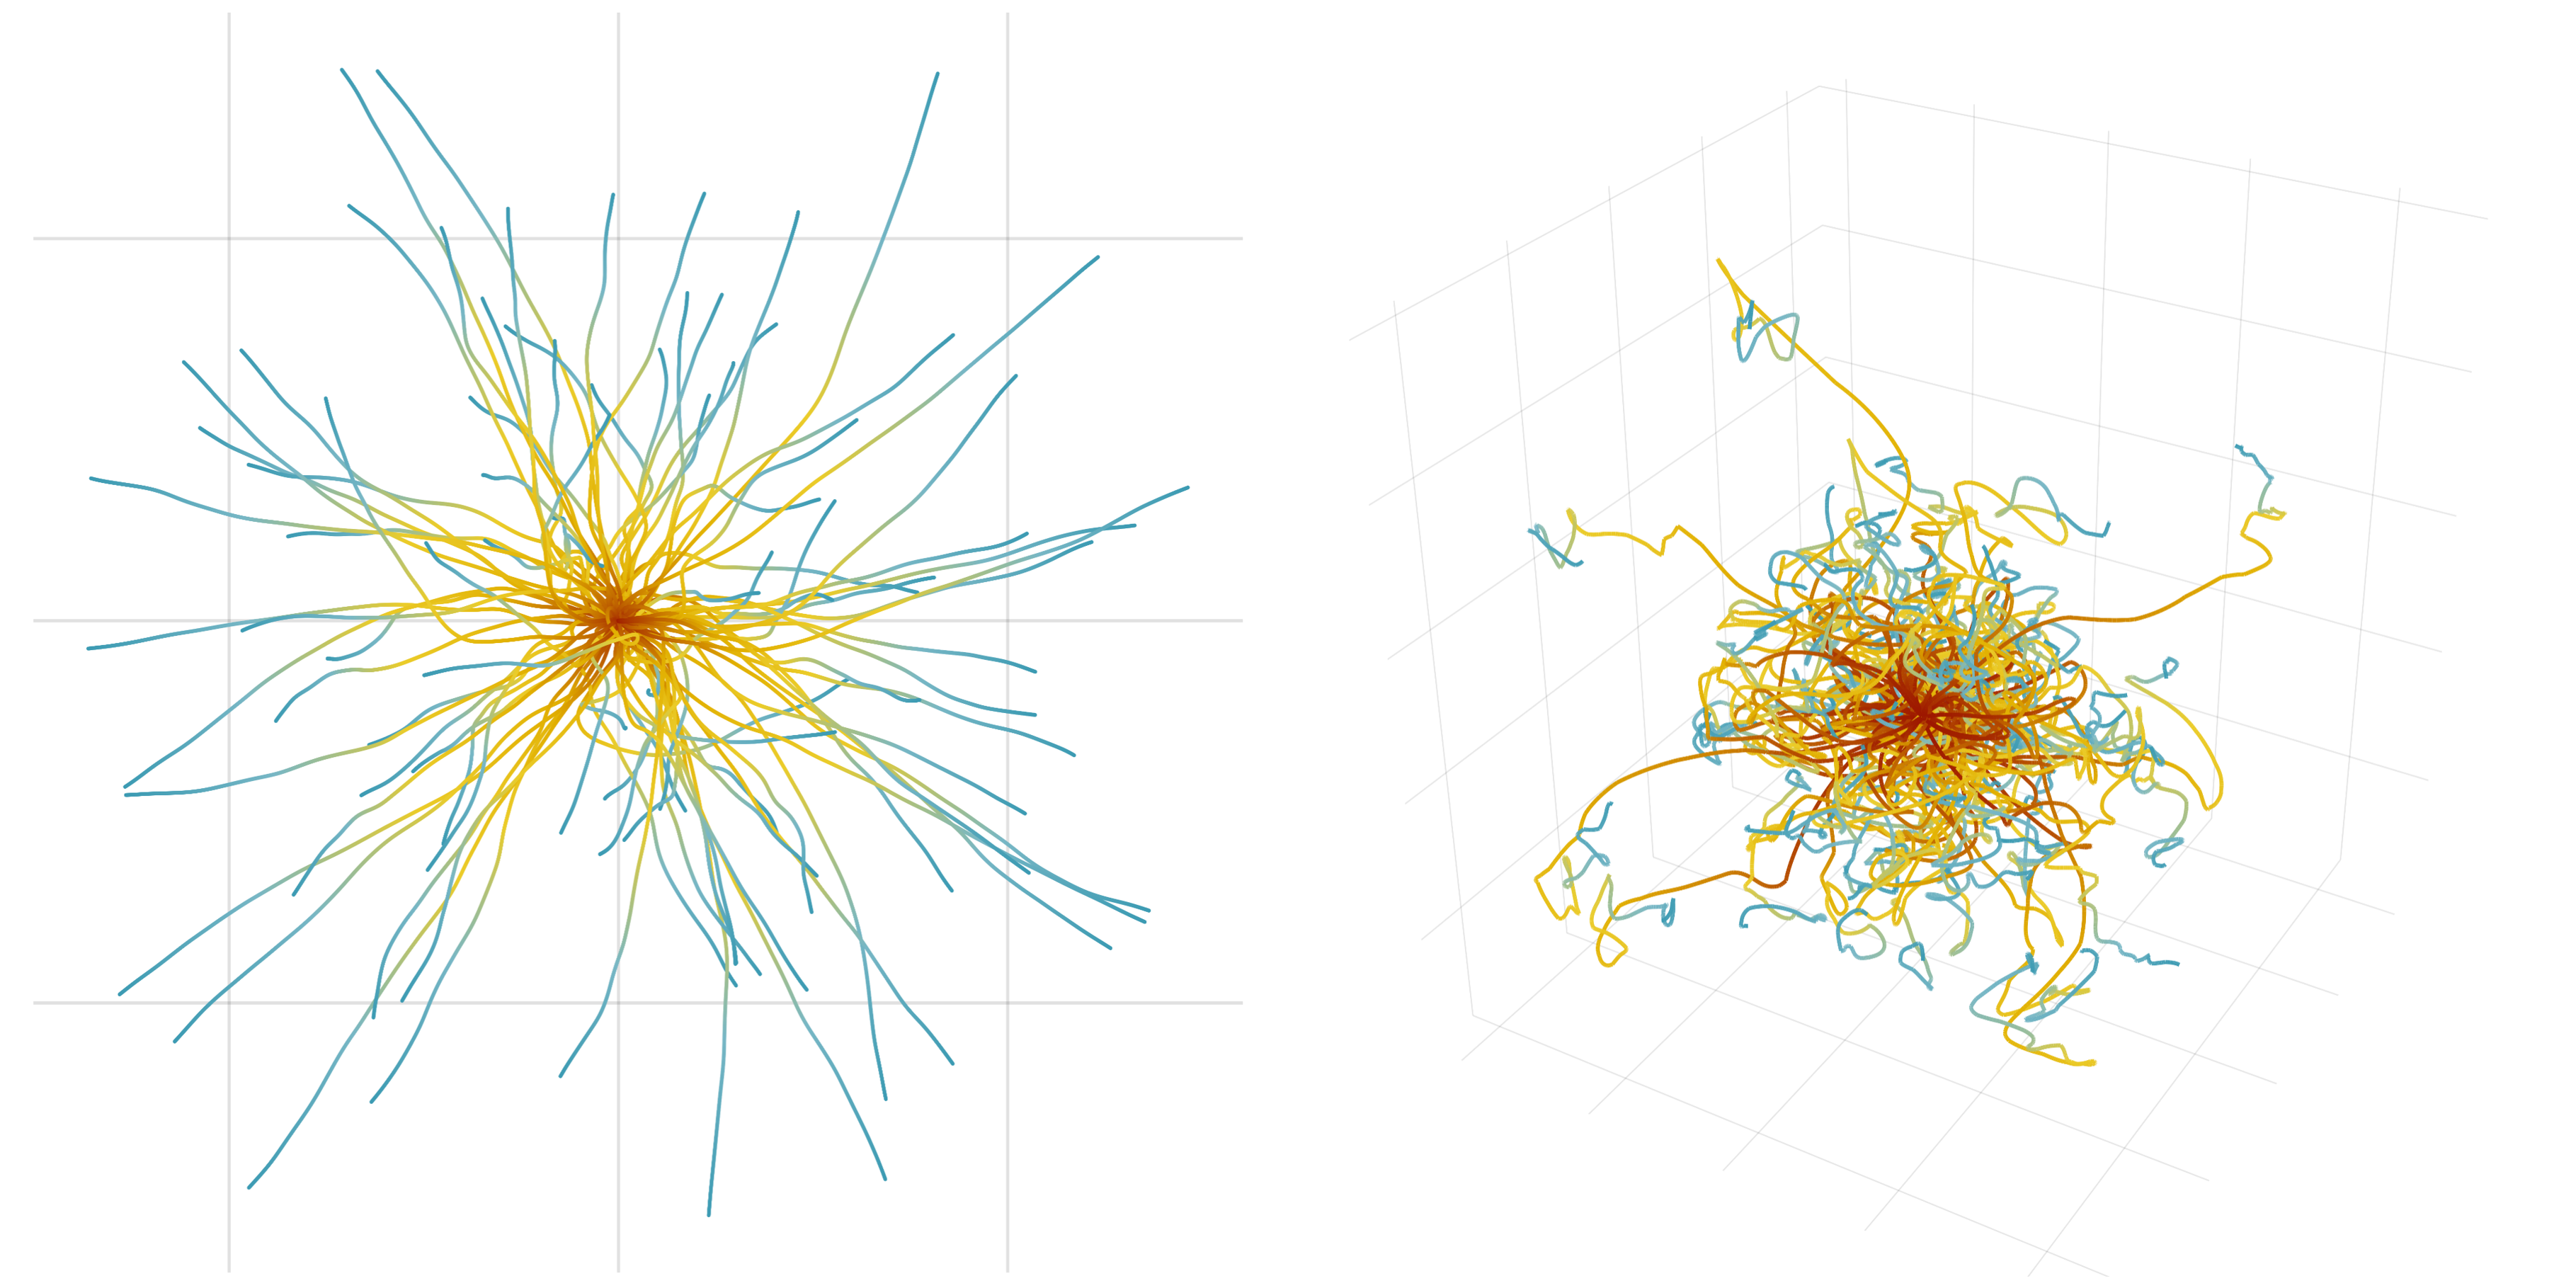
\includegraphics[height=0.7\paperheight]{images/trajectories_cpic.png}} 
    \\[10pt]  
   };
}
\begin{frame}{Outline}
    \begin{center}
        \tableofcontents
    \end{center}
\end{frame}
\setbeamertemplate{background}{}

\setcounter{framenumber}{0}
\setbeamertemplate{footline}[progress bar]
\setbeamercolor{progress bar}{fg=palteal,bg=palteal!40}
\addtobeamertemplate{headline}{}{\vspace{1cm}\hfill\circcounter\hspace*{1cm}}
\addtobeamertemplate{frametitle}{\vspace{-0.8cm}}{}

% %%%%%%%%%%%%%%%%%%%%%%%%%%%%%%%%%%%%%%%%%
% %%%%%%%%%%%%%%%% SECTION %%%%%%%%%%%%%%%%
% %%%%%%%%%%%%%%%%%%%%%%%%%%%%%%%%%%%%%%%%%

% \section{Initial stage of heavy-ion collisions}

% %%%%%%%%%%%%%%%%%%%%%%%%%%%%%%%%%%%%%%%%%
% %%%%%%%%%%%%%%%%% SLIDE %%%%%%%%%%%%%%%%%
% %%%%%%%%%%%%%%%%%%%%%%%%%%%%%%%%%%%%%%%%%

% \begin{frame}
%     \frametitle{Heavy-ion collisions}
%     \framesubtitle{Stages at weak coupling}

%     \begin{center}
%         \begin{tikzpicture}
%             \node[anchor=south west,inner sep=0] at (0,0) {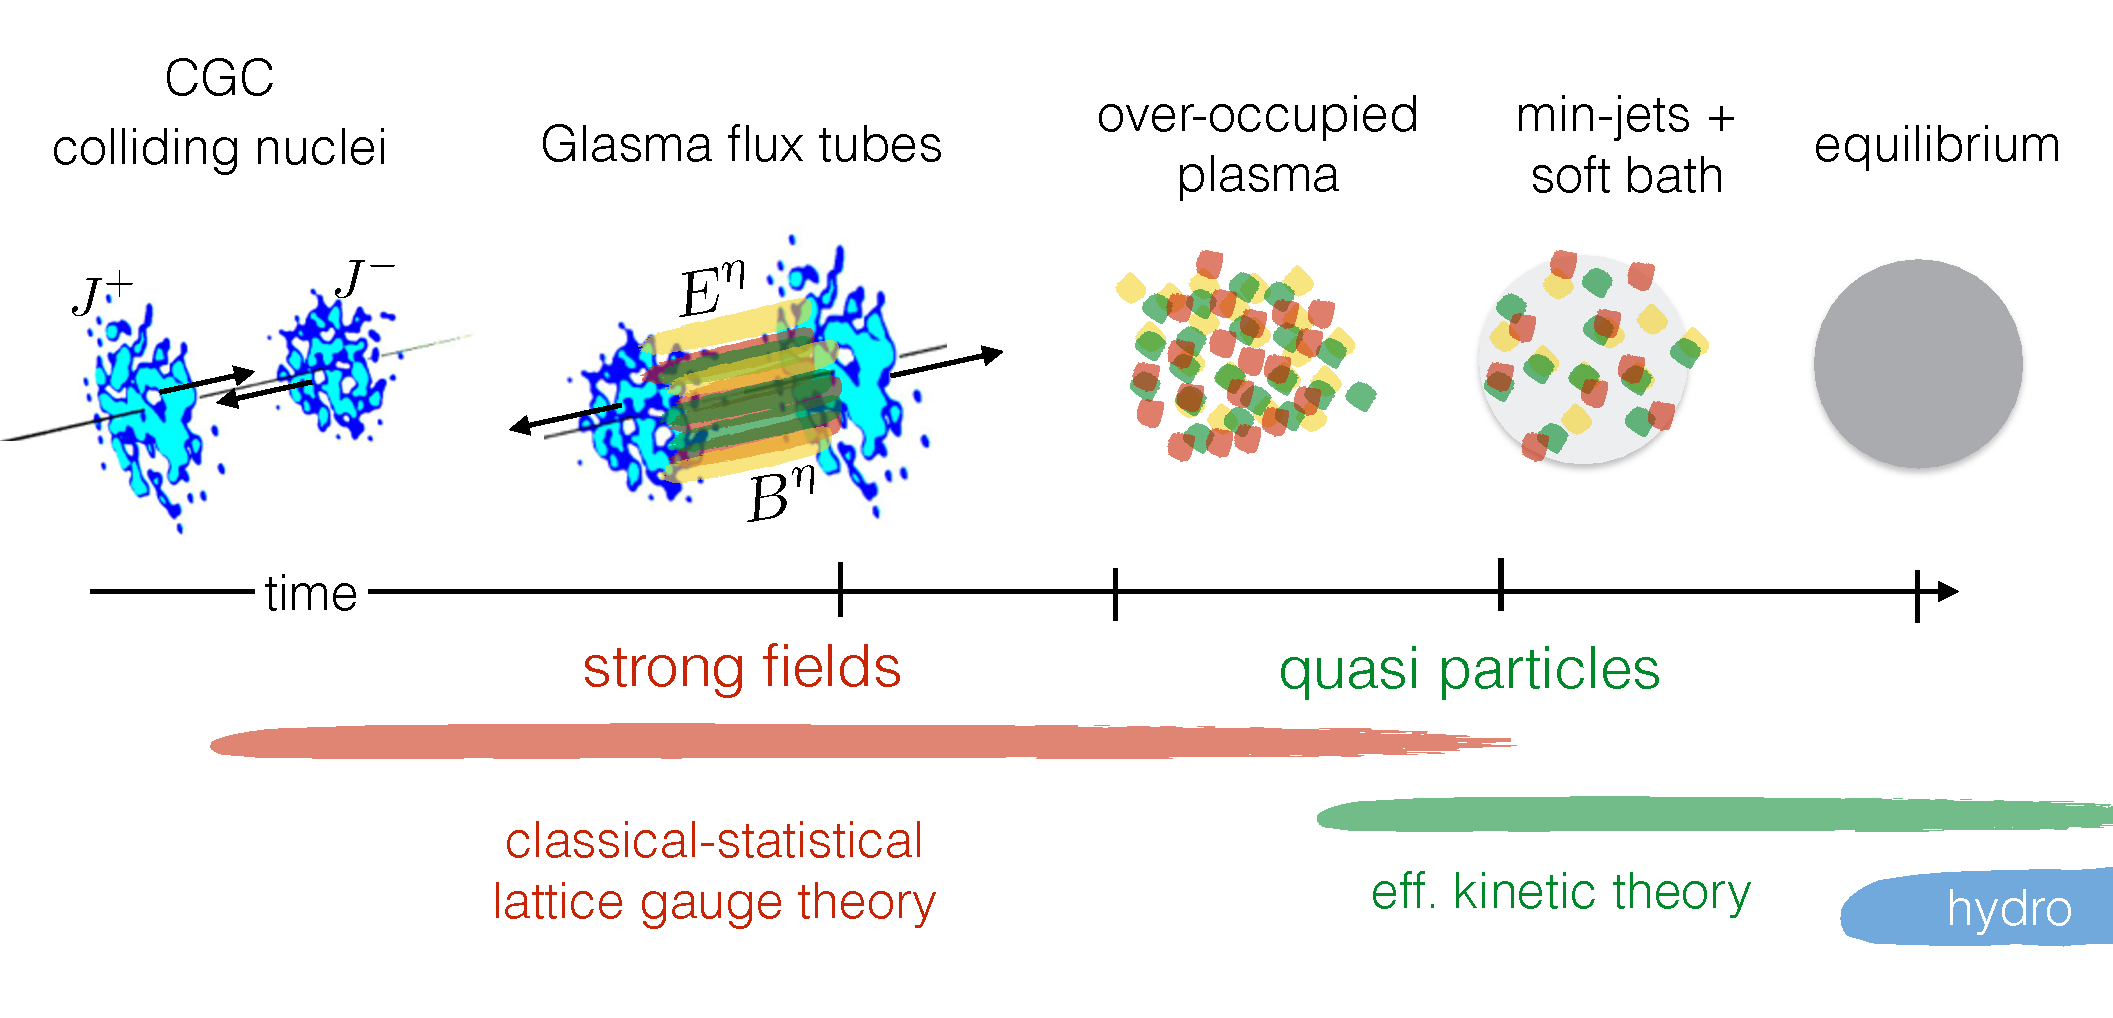
\includegraphics[width=0.8\textwidth]{images/SchlichtingIS2016-pages-cropped.pdf}};
%         \end{tikzpicture}
%     \end{center}
        
%     \blfootnote{\scriptsize Schlichting \href{https://indico.cern.ch/event/469857/contributions/1978347/attachments/1277798/1896654/SchlichtingIS2016.pdf}{{\color{palgold}\texttt{[Initial Stages]$^\text{\tiny\faExternalLink}$}}}}
% \end{frame}

% %%%%%%%%%%%%%%%%%%%%%%%%%%%%%%%%%%%%%%%%%
% %%%%%%%%%%%%%%%%% SLIDE %%%%%%%%%%%%%%%%%
% %%%%%%%%%%%%%%%%%%%%%%%%%%%%%%%%%%%%%%%%%

% \setbeamertemplate{itemize item}{\raisebox{0.2em}{\scalebox{0.7}{${\color{palgold}\blacktriangleright}$}}} 

% \begin{frame}[noframenumbering]
%     \frametitle{Heavy-ion collisions}
%     \framesubtitle{The very early stage}
    
%     \begin{center}
%         \begin{tikzpicture}[]
%             \node[anchor=south west,inner sep=0] at (0,0) {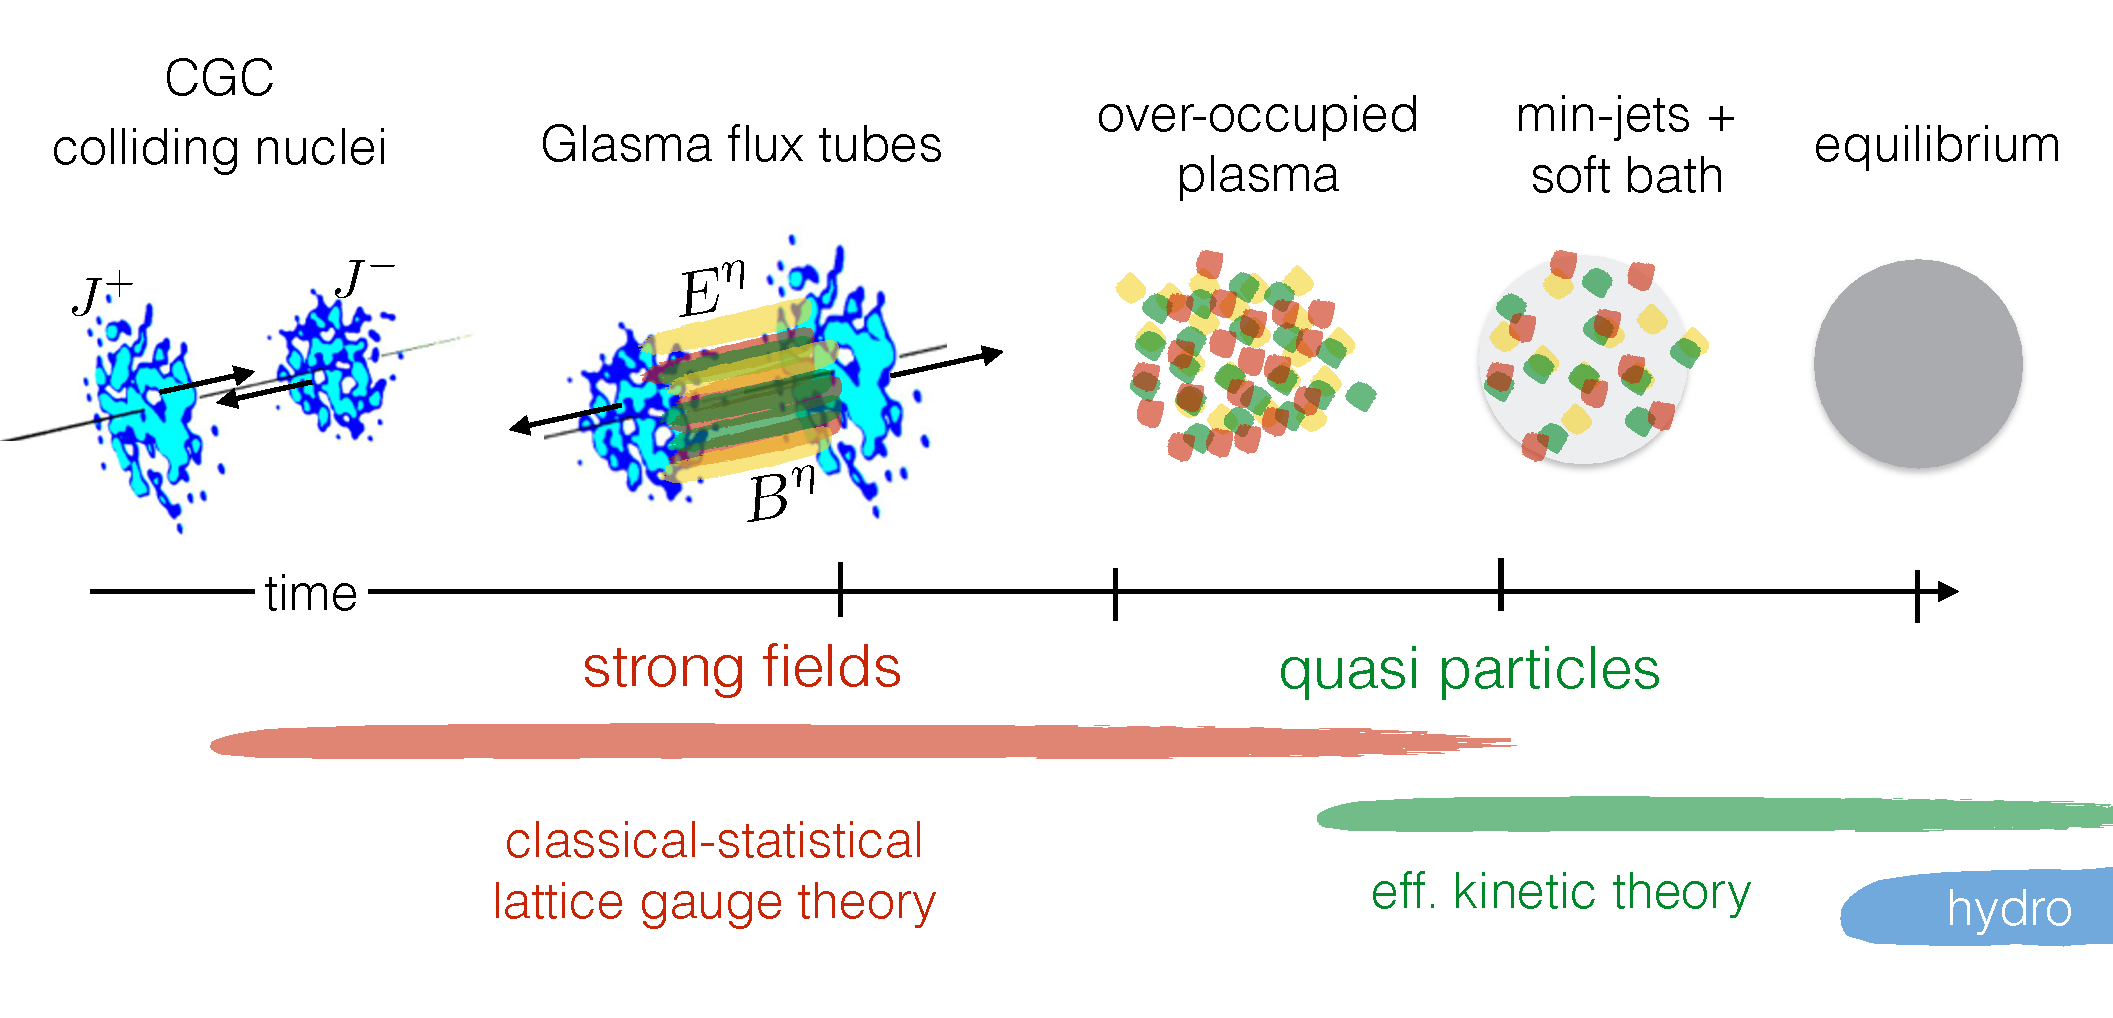
\includegraphics[width=0.8\textwidth]{images/SchlichtingIS2016-pages-cropped.pdf}};
%             \draw<1>[white, fill=white, fill opacity=0.9] (6.3,0) rectangle (\textheight+4.6cm,5.5) node[pos=0.5, anchor=center, xshift=0.03\linewidth,text width=6.8cm,align=center] {{\Large\color{palgold}\bfseries Glasma initial stage}\\[10pt]\begin{itemize}
%                 \footnotesize
%                 \item {\color{normal}Framework}: {\bfseries color glass condensate}
%                 \item {\color{normal}Regime}: {\bfseries weakly coupled} $\alpha_s\ll 1$
%                 \item {\color{normal}Degree of freedom}: {\bfseries gluon fields} $\rightarrow$ occupation $\sim 1/\alpha_s\gg 1$ $\Rightarrow$ {\bfseries classical}
%                 \item {\color{normal}Technique}: real-time classical {\bfseries lattice gauge theory}
%                 \item {\color{normal}Property}: {\bfseries out-of-equilibrium}
%             \end{itemize}
%             };
%             \draw<1>[palgold,thick,fill=palgold,fill opacity=0.1,rounded corners=3pt] (-0.1,0.3) rectangle (\textheight-1.45cm,5.75);
%         \end{tikzpicture}
%     \end{center}
        
%     \blfootnote{\scriptsize Lappi \href{https://arxiv.org/abs/hep-ph/0606207}{{\color{palgold}\texttt{[hep-ph/0606207]}$^\text{\tiny\faExternalLink}$}}, Gelis \href{https://arxiv.org/abs/1211.3327}{{\color{palgold}\texttt{[1211.3327]}$^\text{\tiny\faExternalLink}$}}}
% \end{frame}

% %%%%%%%%%%%%%%%%%%%%%%%%%%%%%%%%%%%%%%%%%
% %%%%%%%%%%%%%%%% SECTION %%%%%%%%%%%%%%%%
% %%%%%%%%%%%%%%%%%%%%%%%%%%%%%%%%%%%%%%%%%

% \section{Glasma}

% %%%%%%%%%%%%%%%%%%%%%%%%%%%%%%%%%%%%%%%%%
% %%%%%%%%%%%%%%%%% SLIDE %%%%%%%%%%%%%%%%%
% %%%%%%%%%%%%%%%%%%%%%%%%%%%%%%%%%%%%%%%%%

% \setbeamertemplate{background}{
% \tikz[overlay,remember picture] \node[opacity=0.1, at=(current page.center), align=center] {\\[10pt]
% {\transparent{0.2}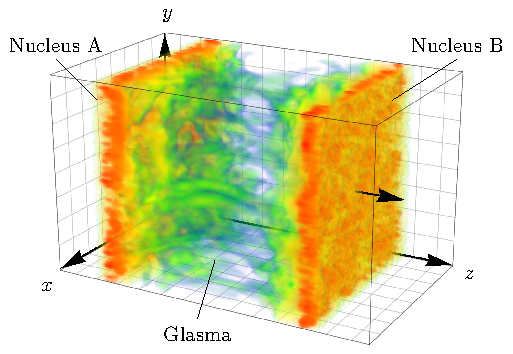
\includegraphics[height=0.8\paperheight]{images/fig1_overview.pdf}}};
% }
% \begin{frame}[plain,noframenumbering]{}
%     \begin{center}
%         \vspace{1cm}
%         {\large\color{normal}Initial stage of pre-equilibrium}\\[0.3cm]
%         {\huge\color{destacado}The glasma}
%     \end{center}
% \end{frame}
% \setbeamertemplate{background}{}

% %%%%%%%%%%%%%%%%%%%%%%%%%%%%%%%%%%%%%%%%%
% %%%%%%%%%%%%%%%%% SLIDE %%%%%%%%%%%%%%%%%
% %%%%%%%%%%%%%%%%%%%%%%%%%%%%%%%%%%%%%%%%%

% \setbeamertemplate{background}{
% \tikz[overlay,remember picture] \node[at=(current page.center), align=center] {\\[10pt]
% {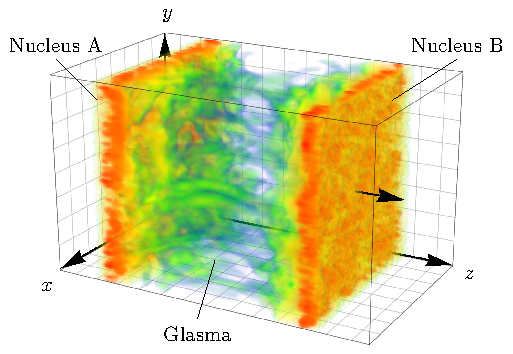
\includegraphics[height=0.7\paperheight]{images/fig1_overview.pdf}}};
% }
% \begin{frame}[plain,noframenumbering]
%     \frametitle{\\ Glasma color fields}
%     \blfootnote{\scriptsize Ipp, Müller  \href{https://arxiv.org/abs/1703.00017}{{\color{palgold}\texttt{[1703.00017]}$^\text{\tiny\faExternalLink}$}}}
% \end{frame}
% \setbeamertemplate{background}{}

% %%%%%%%%%%%%%%%%%%%%%%%%%%%%%%%%%%%%%%%%%
% %%%%%%%%%%%%%% SUBSECTION %%%%%%%%%%%%%%%
% %%%%%%%%%%%%%%%%%%%%%%%%%%%%%%%%%%%%%%%%%

% \subsection{Color glass condensate}

% %%%%%%%%%%%%%%%%%%%%%%%%%%%%%%%%%%%%%%%%%
% %%%%%%%%%%%%%%%%% SLIDE %%%%%%%%%%%%%%%%%
% %%%%%%%%%%%%%%%%%%%%%%%%%%%%%%%%%%%%%%%%%

% \setbeamertemplate{itemize item}{\raisebox{0.2em}{\scalebox{0.7}{${\color{normal}\blacktriangleright}$}}} 

% \begin{frame}
%     \frametitle{Color glass condensate}
%     \framesubtitle{Effective field theory of QCD at high energies}
%     \vspace{-10pt}
%     \begin{columns}[onlytextwidth,t]
%        \column{.033\textwidth}
%        \column{.45\textwidth}

%             \begin{itemize}
%                 \footnotesize\color{lightgray}
%                 \setbeamertemplate{itemize item}{\raisebox{0.2em}{\scalebox{0.6}{${\color{lightgray}\blacktriangleright}$}}}
%                 \item High-energy nucleus $\rightarrow$ mostly {\color{palviolet}soft gluons}
%             \end{itemize}

%             \vspace{5pt}
%             \hspace{10pt}
%             \begin{tikzpicture}[]
%                 \node[anchor=south west,inner sep=0] at (0,0) {\includegraphics[width=0.7\textwidth]{images/CFNS_talk_Salazar-3_crop_edit_final_v2.png}};
%                 \draw<1>[palviolet,thin,fill=palviolet,fill opacity=0.1,rounded corners=3pt] (2.2, 0) rectangle (4.8, 4.9);
%             \end{tikzpicture}
%         \column{.033\textwidth}
%         \column{.45\textwidth}
           
%             \begin{custombox}{Color glass condensate}{lightgray}
%                 \small
%                 \begin{varwidth}{0.88\textwidth}
%                 \begin{itemize}
%                     \setbeamertemplate{itemize item}{\raisebox{0.2em}{\scalebox{0.7}{${\color{palviolet}\blacktriangleright}$}}} 
%                     \item Soft partons $\rightarrow$ {\color{palviolet}\bfseries gauge fields $\boldsymbol{A^\mu}$}
%                     \setbeamertemplate{itemize item}{\raisebox{0.2em}{\scalebox{0.7}{${\color{palteal}\blacktriangleright}$}}} 
%                     \item Hard partons $\rightarrow$ {\color{palteal}\bfseries color current $\boldsymbol{J^\mu}$}
%                 \end{itemize}
%                 \end{varwidth}
%             \end{custombox}

%             \begin{itemize}
%                 \footnotesize\color{lightgray}
%                 \setbeamertemplate{itemize item}{\raisebox{0.2em}{\scalebox{0.6}{${\color{lightgray}\blacktriangleright}$}}}
%                 \item Classical {\color{palviolet}gluon fields} $\rightarrow$ produced\\ by color {\color{pallightblue}nucleus current}
%             \end{itemize}
%             \begin{itemize}
%                 \item Classical Yang-Mills equations
%             \end{itemize}
%             \vspace{25pt}
%             \renewcommand{\eqnhighlightheight}{\vphantom{\mathcal{D}_\mu}\mathstrut}\begin{equation*}
%                 \hspace{0pt}\eqnmark[normal]{dmu}{\mathscr{D}_\mu}\hspace{-3pt}\eqnmark[normal]{fmunu}{F^{\mu\nu}}\hspace{-3pt}={\color{palteal}\boldsymbol{J^\nu}}{\color{lightgray}\rightarrow\text{need input }\,{\color{palteal}J^\nu}} 
%                 \end{equation*}
%                 \annotate[yshift=-0.7em]{below, right}{dmu}{\scriptsize $\partial_\mu-\mathrm{i}g{\color{palviolet}\boldsymbol{A_\mu}}$}
%                 \annotate[yshift=1.2em]{above}{fmunu}{\scriptsize $\partial_\mu{\color{palviolet}\boldsymbol{A_\nu}}-\partial_\nu{\color{palviolet}\boldsymbol{A_\mu}}-\mathrm{i}g[{\color{palviolet}\boldsymbol{A_\mu}},{\color{palviolet}\boldsymbol{A_\nu}}]$}
              
%         \column{.033\textwidth}
%     \end{columns}
%     \blfootnote{\scriptsize Gelis, Iancu, Jalilian-Marian, Venugopalan \href{https://arxiv.org/abs/1002.0333}{{\color{palgold}\texttt{[1002.0333]}$^\text{\tiny\faExternalLink}$}}}
% \end{frame}

% %%%%%%%%%%%%%%%%%%%%%%%%%%%%%%%%%%%%%%%%%
% %%%%%%%%%%%%%%%%% SLIDE %%%%%%%%%%%%%%%%%
% %%%%%%%%%%%%%%%%%%%%%%%%%%%%%%%%%%%%%%%%%

% \begin{frame}
%     \frametitle{Color glass condensate}
%     \framesubtitle{MV model for large nuclei}
%     \vspace{-10pt}
%     \begin{columns}[onlytextwidth,t]
%         \column{.033\textwidth}
%         \column{.4\textwidth}

%         \begin{itemize}
%             \footnotesize\color{lightgray}
%             \setbeamertemplate{itemize item}{\raisebox{0.2em}{\scalebox{0.6}{${\color{lightgray}\blacktriangleright}$}}}
%             \item Color charge distribution in a nucleus \\ at high energy $\rightarrow$ thin {\color{palviolet}color sheet}
%         \end{itemize}

%         \begin{figure}
%             \centering
%             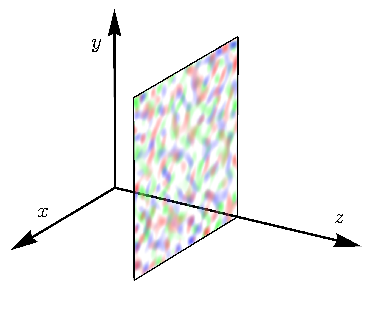
\includegraphics[width=0.9\textwidth]{images/sheets1.pdf}
%         \end{figure}
%        \column{.033\textwidth}
%        \column{.5\textwidth}
%         \begin{custombox}{McLerran Venugopalan model}{lightgray}
%             \small
%             \begin{varwidth}{0.95\textwidth}
%             \begin{itemize}
%                 \setbeamertemplate{itemize item}{\raisebox{0.2em}{\scalebox{0.7}{${\color{palgold}\blacktriangleright}$}}} 
%                 \item {\color{palgold}\bfseries Color charge} $\color{palgold}\boldsymbol{\rho}$ $\rightarrow$ Gaussian probability
%             \end{itemize}
%             \end{varwidth}
%         \end{custombox}

%         \begin{itemize}
%             \footnotesize\color{lightgray}
%             \setbeamertemplate{itemize item}{\raisebox{0.2em}{\scalebox{0.6}{${\color{lightgray}\blacktriangleright}$}}}
%             \item {\color{palteal}Color current} of nucleus $\rightarrow$ generated\\ by {\color{palgold} color charge} density
%         \end{itemize}
%         \begin{itemize}
%             \item {\bfseries\color{palgold} MV model} for color charges ${\color{palgold}\boldsymbol{\rho}}$
%         \end{itemize}
%         \vspace{5pt}
%         \renewcommand{\eqnhighlightheight}{\vphantom{\mathcal{D}_\mu}\mathstrut}\begin{equation*}
%             \big\langle{\color{palgold}\boldsymbol{\rho}}(\vec{x}_\perp){\color{palgold}\boldsymbol{\rho}}(\vec{y}_\perp)\big\rangle\propto(\hspace{-3pt}\eqnmark[normal]{g2mu}{{\color{palviolet}\boldsymbol{g^2\mu}}}\hspace{-3pt})^2\delta^{(2)}(\vec{x}_\perp-\vec{y}_\perp)
%             \end{equation*}
%             \annotate[yshift=-0.7em]{below, right}{g2mu}{\scriptsize $\propto{\color{palviolet}\boldsymbol{Q_s}}$}
%             \vspace{5pt}
%             \begin{itemize}
%                 \item {\color{palviolet}\bfseries Saturation momentum $\boldsymbol{Q_s}$} \\{\scriptsize\color{lightgray} $Q_s\approx 2\,\mathrm{GeV}$ at LHC central collisions}
%             \end{itemize}    
              
%         \column{.033\textwidth}
%     \end{columns}
%     \blfootnote{\scriptsize McLerran, Venugopalan \href{https://arxiv.org/abs/hep-ph/9309289}{{\color{palgold}\texttt{[hep-ph/9309289]}$^\text{\tiny\faExternalLink}$}}, Müller \href{https://arxiv.org/abs/1904.04267}{{\color{palviolet}\texttt{[1904.04267]}$^\text{\tiny\faExternalLink}$}}}
% \end{frame}


% %%%%%%%%%%%%%%%%%%%%%%%%%%%%%%%%%%%%%%%%%
% %%%%%%%%%%%%%% SUBSECTION %%%%%%%%%%%%%%%
% %%%%%%%%%%%%%%%%%%%%%%%%%%%%%%%%%%%%%%%%%

% \subsection{Features of the glasma}

% %%%%%%%%%%%%%%%%%%%%%%%%%%%%%%%%%%%%%%%%%
% %%%%%%%%%%%%%%%%% SLIDE %%%%%%%%%%%%%%%%%
% %%%%%%%%%%%%%%%%%%%%%%%%%%%%%%%%%%%%%%%%%

% \begin{frame}
%     \frametitle{Collision of two nuclei}
%     \framesubtitle{How to construct the glasma fields}
%     \vspace{-10pt}
%     \begin{columns}[onlytextwidth,t]
%         \column{.033\textwidth}
%         \column{.4\textwidth}

%         \begin{itemize}
%             \item Light-cone diagram of collision\\
%             {\scriptsize\color{lightgray} Light-cone coordinates $x^\pm=t\pm z$}
%         \end{itemize}
%         \begin{tikzpicture}[]
%             \node[anchor=south west,inner sep=0] at (0,0) {\includegraphics[width=\textwidth]{images/spacetb.eps}};
%             \node[isosceles triangle,
%                 isosceles triangle apex angle=90,
%                 draw=red,opacity=0.05,
%                 fill=red,fill opacity=0.1,
%                 minimum size =2cm] (T90)at (1.8,2.2){};
%             \node[isosceles triangle,
%                 isosceles triangle apex angle=90,
%                 draw=red,opacity=0.05,
%                 fill=red,fill opacity=0.1,
%                 rotate=180,
%                 minimum size =2cm] (T90)at (4.25,2.2){};
%             \node[isosceles triangle,
%                 isosceles triangle apex angle=90,
%                 draw=palviolet,opacity=0.05,line width=1pt,
%                 fill=palviolet,fill opacity=0.1,
%                 rotate=270,
%                 minimum size =2cm] (T90)at (3.03,3.43){};
%         \end{tikzpicture}

%        \column{.033\textwidth}
%        \column{.5\textwidth}
%         \begin{custombox}{{\normalsize CGC fields} {\tiny (regions 1, 2)}}{red}
%             \small
%             \begin{varwidth}{0.9\textwidth}
%             \begin{itemize}
%                 \setbeamertemplate{itemize item}{\raisebox{0.2em}{\scalebox{0.7}{${\color{red}\blacktriangleright}$}}} 
%                 \footnotesize
%                 \item Analytical {\color{red}pure gauge} fields before collision
%             \end{itemize}
%             \end{varwidth}
%         \end{custombox}

%         \begin{custombox}{{\normalsize Initial condition} {\tiny (along light-cone)}}{normal}
%             \small
%             \begin{varwidth}{0.9\textwidth}
%             \begin{itemize}
%                 \setbeamertemplate{itemize item}{\raisebox{0.2em}{\scalebox{0.7}{${\color{normal}\blacktriangleright}$}}} 
%                 \footnotesize
%                 \item Match CGC fields on the light cone
%                 \item Impose boost-invariance\\
%                 {\tiny\color{lightgray} Milne coordinates {\color{Blue}$\tau=\sqrt{x^+x^-}$} and {\color{ForestGreen}$\eta=\mathrm{ln}(x^+/x^-)$}}
%             \end{itemize}
%             \end{varwidth}
%         \end{custombox}

%         \begin{custombox}{{\normalsize Glasma fields} {\tiny (region 3)}}{palviolet}
%             \small
%             \begin{varwidth}{0.9\textwidth}
%             \begin{itemize}
%                 \setbeamertemplate{itemize item}{\raisebox{0.2em}{\scalebox{0.7}{${\color{palviolet}\blacktriangleright}$}}} 
%                 \footnotesize
%                 \item Solve numerically YM equations
%                 \item Code \href{https://gitlab.com/openpixi/curraun}{\color{palviolet}\texttt{gitlab.com/openpixi/curraun}$^\text{\tiny\faGitlab}$}
%             \end{itemize}
%             \end{varwidth}
%         \end{custombox}
%         \column{.033\textwidth}
%     \end{columns}
%     \blfootnote{\scriptsize Lappi \href{https://arxiv.org/abs/hep-ph/0602189}{{\color{palgold}\texttt{[hep-ph/0602189]}$^\text{\tiny\faExternalLink}$}}}
% \end{frame}

% %%%%%%%%%%%%%%%%%%%%%%%%%%%%%%%%%%%%%%%%%
% %%%%%%%%%%%%%%%%% SLIDE %%%%%%%%%%%%%%%%%
% %%%%%%%%%%%%%%%%%%%%%%%%%%%%%%%%%%%%%%%%%

% \begin{frame}
%     \frametitle{Features of the glasma}
%     % \framesubtitle{Flux tubes, strong fields, correlation domains}
%     % \vspace{-10pt}
%     \begin{columns}[onlytextwidth,t]
%         \column{.025\textwidth}
%         \column{.3\textwidth}

%         \begin{custombox}{{\normalsize Flux tubes}}{palteal}
%             \begin{varwidth}{0.95\columnwidth}
%             \begin{itemize}
%                 \setbeamertemplate{itemize item}{\raisebox{0.2em}{\scalebox{0.7}{${\color{palteal}\blacktriangleright}$}}} 
%                 \scriptsize
%                 \item Initially only longitudinal electric and magnetic fields
%             \end{itemize}
%             \end{varwidth}
%         \end{custombox}

%         \vspace{5pt}
%         \begin{center}
%             \begin{figure}
%                 \centering
%                 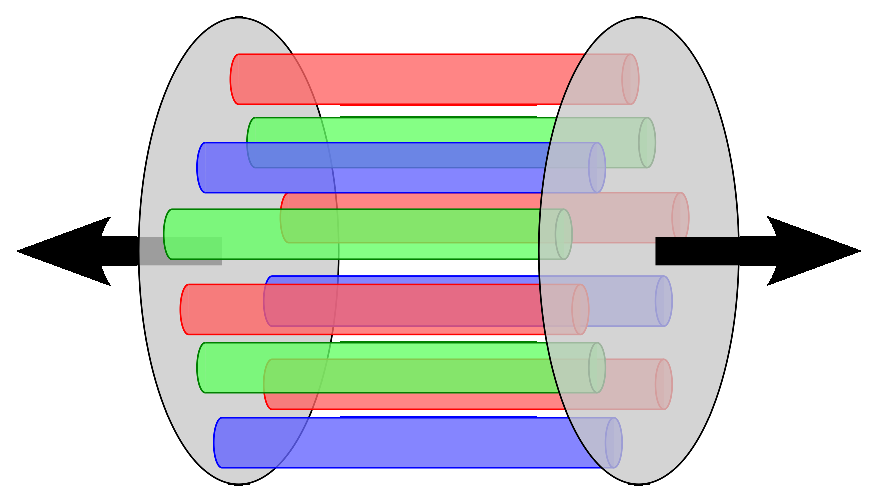
\includegraphics[width=0.9\textwidth]{images/glasma.eps}
%             \end{figure}
%         \end{center}

%        \column{.025\textwidth}
%        \column{.3\textwidth}
%        \begin{custombox}{{\normalsize Strong fields}}{palviolet}
%             \begin{varwidth}{0.95\columnwidth}
%             \begin{itemize}
%                 \setbeamertemplate{itemize item}{\raisebox{0.2em}{\scalebox{0.7}{${\color{palviolet}\blacktriangleright}$}}} 
%                 \scriptsize
%                 \item Strong longitudinal fields, dilute after $\tau\sim 1/Q_s$
%             \end{itemize}
%             \end{varwidth}
%         \end{custombox}
        
%         \begin{center}
%             \begin{figure}
%                 \centering
%                 \includegraphics[width=0.9\textwidth]{images/components.eps}
%             \end{figure}
%         \end{center}

%         \column{.025\textwidth}
%         \column{.3\textwidth}
%         \begin{custombox}{{\normalsize Correlation domains}}{palgold}
%             \begin{varwidth}{0.95\columnwidth}
%             \begin{itemize}
%                 \setbeamertemplate{itemize item}{\raisebox{0.2em}{\scalebox{0.7}{${\color{palgold}\blacktriangleright}$}}} 
%                 \scriptsize
%                 \item Fields correlated inside flux tubes of size $\sim 1/Q_s$ 
%             \end{itemize}
%             \end{varwidth}
%         \end{custombox}
        
%         \begin{center}
%             \begin{figure}
%                 \centering
%                 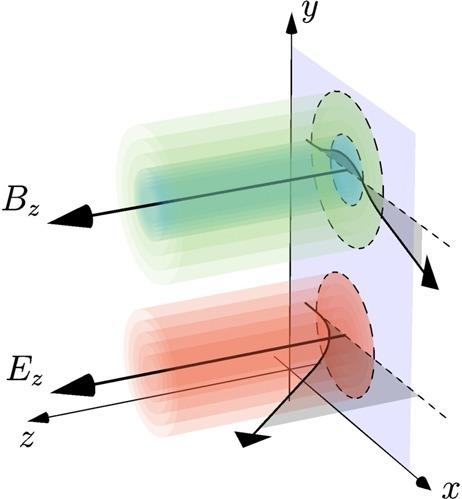
\includegraphics[width=0.7\textwidth]{images/1-s2.0-S0370269320306134-gr003_lrg.jpg}
%             \end{figure}
%         \end{center}

%         \column{.025\textwidth}
%     \end{columns}
%         \begin{itemize}
%             \setbeamertemplate{itemize item}{\raisebox{0.2em}{\scalebox{0.7}{${\color{destacado}\blacktriangleright}$}}} 
%             \item \begin{center}Heavy quarks and jets are sensitive to the properties of the glasma fields\end{center}
%         \end{itemize}
%     \blfootnote{\scriptsize Fukushima \href{https://arxiv.org/abs/1603.02340}{{\color{palteal}\texttt{[1603.02340]}$^\text{\tiny\faExternalLink}$}}, Lappi \href{https://arxiv.org/abs/hep-ph/0606207}{{\color{palviolet}\texttt{[hep-ph/0606207]}$^\text{\tiny\faExternalLink}$}}, Ipp, Müller, Schuh \href{https://arxiv.org/abs/2009.14206}{{\color{palgold}\texttt{[2009.14206]}$^\text{\tiny\faExternalLink}$}}}
% \end{frame}

% %%%%%%%%%%%%%%%%%%%%%%%%%%%%%%%%%%%%%%%%%
% %%%%%%%%%%%%%%%% SECTION %%%%%%%%%%%%%%%%
% %%%%%%%%%%%%%%%%%%%%%%%%%%%%%%%%%%%%%%%%%

% \section{Heavy quarks in glasma}

% %%%%%%%%%%%%%%%%%%%%%%%%%%%%%%%%%%%%%%%%%
% %%%%%%%%%%%%%%%%% SLIDE %%%%%%%%%%%%%%%%%
% %%%%%%%%%%%%%%%%%%%%%%%%%%%%%%%%%%%%%%%%%

% \setbeamertemplate{background}{
% \tikz[overlay,remember picture] \node[opacity=0.1, at=(current page.center), align=center] {\\[10pt]
% {\transparent{0.1}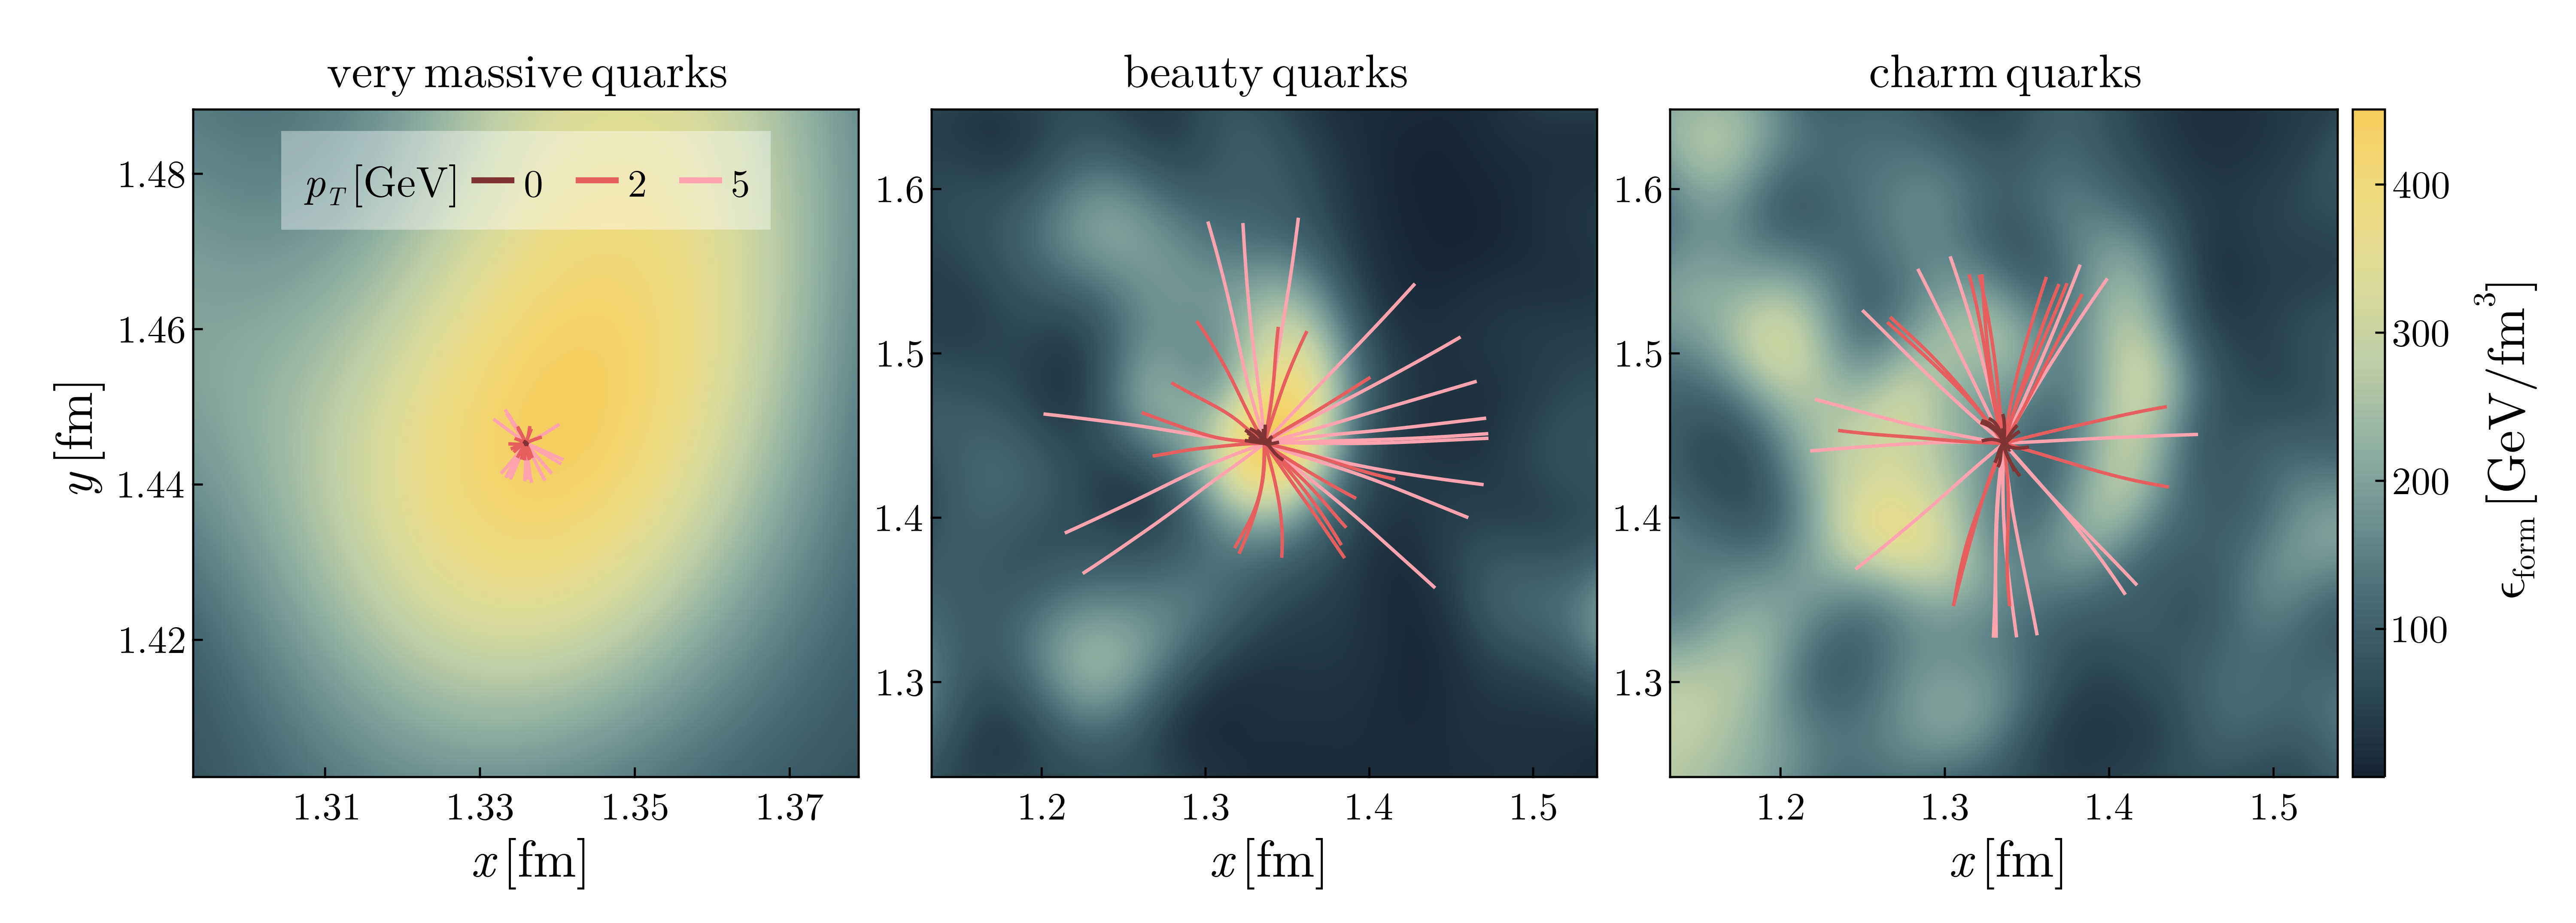
\includegraphics[height=0.6\paperheight]{images/hqs_flux_tubes_background+hqs.png}}};
% }
% \setbeamertemplate{itemize item}{\raisebox{0.2em}{\scalebox{0.7}{${\color{normal}\blacktriangleright}$}}} 
% \begin{frame}[plain,noframenumbering]{}
%     \begin{center}
%         \vspace{1cm}
%         {\large\color{normal}Probes of the initial stage of pre-equilibrium}\\[0.3cm]
%         {\huge\color{destacado}Heavy quarks in glasma}\\[0.3cm]
%     \end{center}
% \end{frame}
% \setbeamertemplate{background}{}

% %%%%%%%%%%%%%%%%%%%%%%%%%%%%%%%%%%%%%%%%%
% %%%%%%%%%%%%%%%%% SLIDE %%%%%%%%%%%%%%%%%
% %%%%%%%%%%%%%%%%%%%%%%%%%%%%%%%%%%%%%%%%%

% \setbeamertemplate{background}{
% \tikz[overlay,remember picture] \node[at=(current page.center), align=center] {\\[20pt]
% {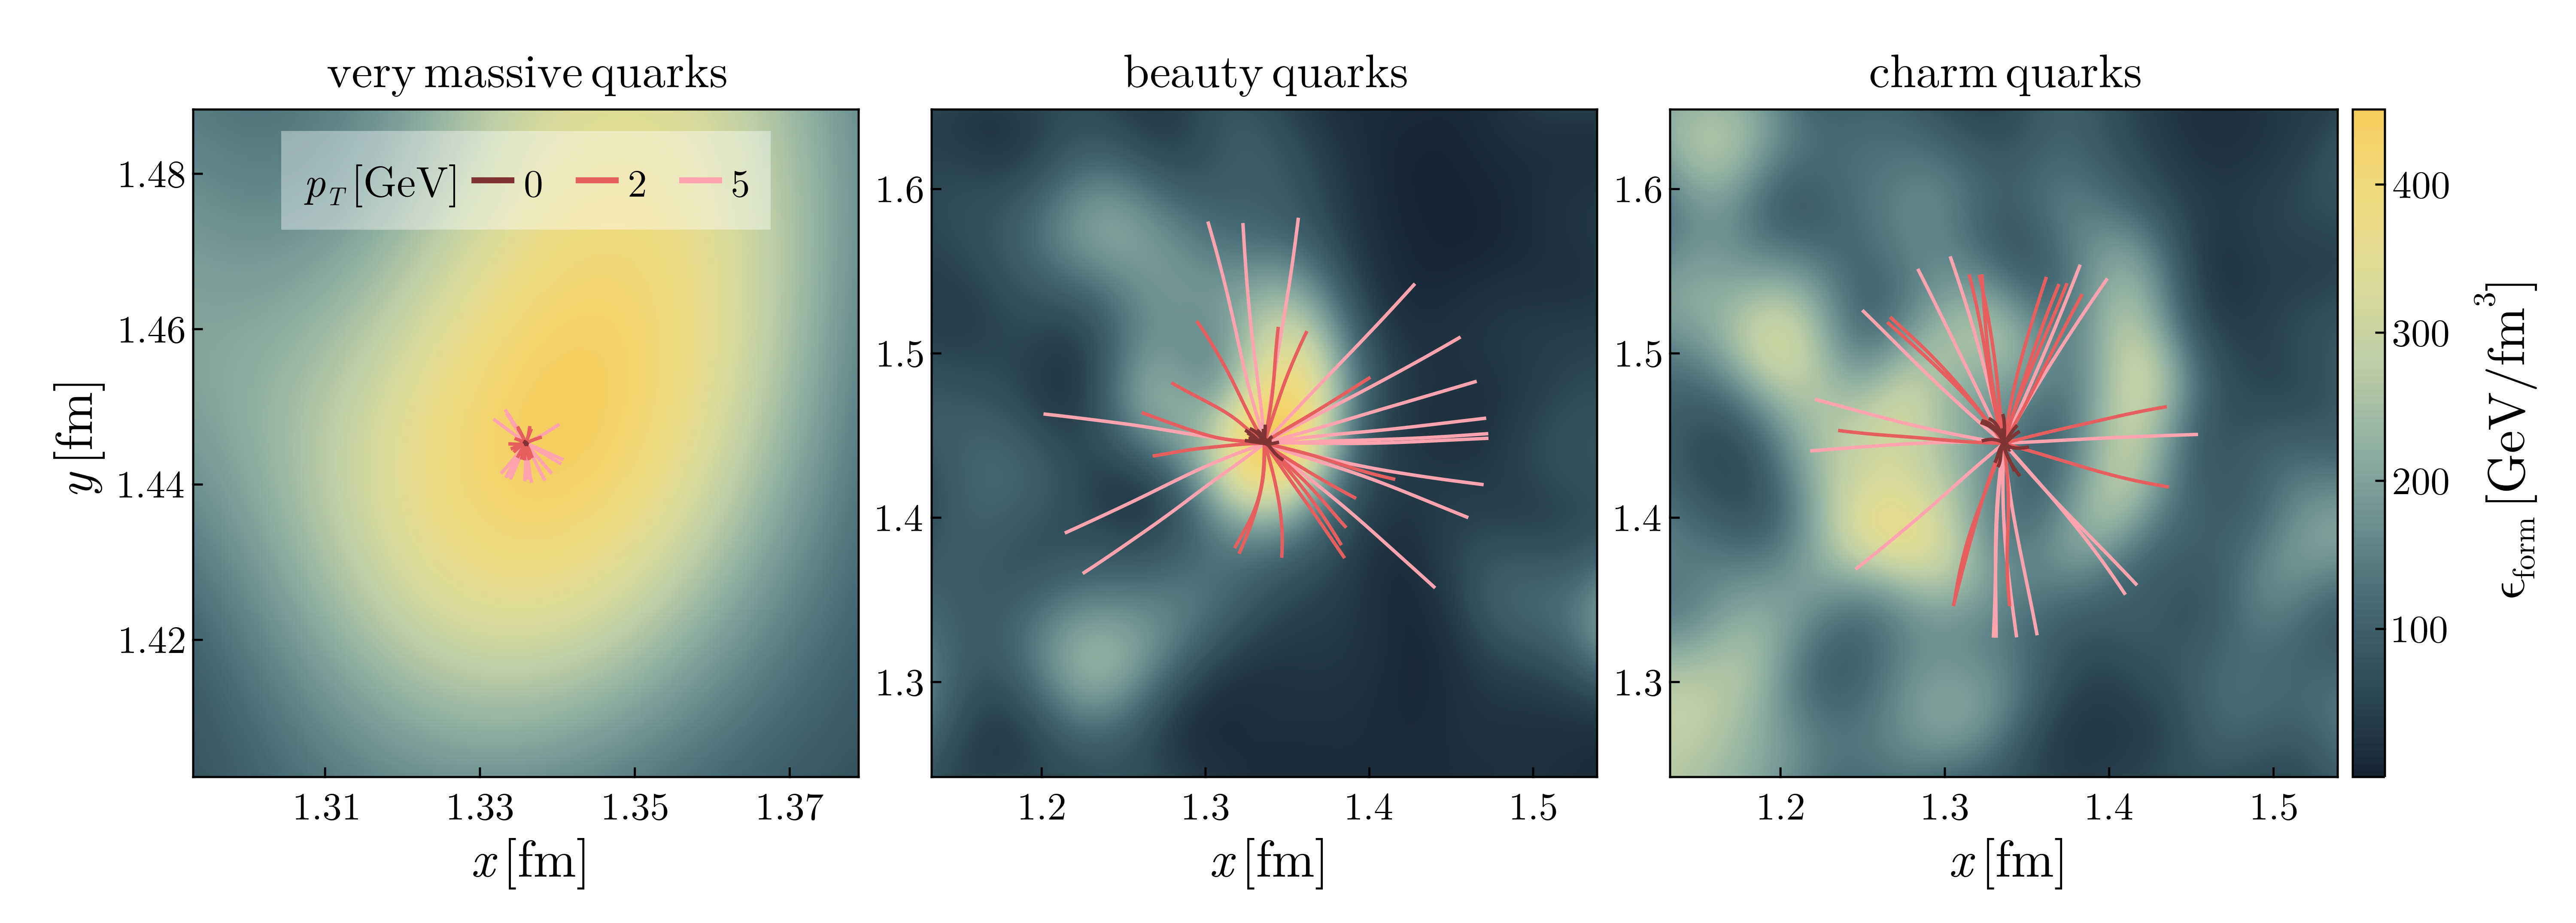
\includegraphics[height=0.6\paperheight]{images/hqs_flux_tubes_background+hqs.png}}};
% }
% \setbeamertemplate{itemize item}{\raisebox{0.2em}{\scalebox{0.7}{${\color{normal}\blacktriangleright}$}}} 
% \begin{frame}[plain,noframenumbering]{}
%     \frametitle{\\ Heavy quarks in glasma}
%     \framesubtitle{Probing the glasma correlation domains}
%     \blfootnote{\scriptsize Avramescu, Băran, Greco, Ipp, Müller, Ruggieri  \href{https://arxiv.org/abs/2303.05599}{{\color{palgold}\texttt{[2303.05599]}$^\text{\tiny\faExternalLink}$}}}
% \end{frame}
% \setbeamertemplate{background}{}

% %%%%%%%%%%%%%%%%%%%%%%%%%%%%%%%%%%%%%%%%%
% %%%%%%%%%%%%%% SUBSECTION %%%%%%%%%%%%%%%
% %%%%%%%%%%%%%%%%%%%%%%%%%%%%%%%%%%%%%%%%%

% \subsection{Transport equations}

% %%%%%%%%%%%%%%%%%%%%%%%%%%%%%%%%%%%%%%%%%
% %%%%%%%%%%%%%%%%% SLIDE %%%%%%%%%%%%%%%%%
% %%%%%%%%%%%%%%%%%%%%%%%%%%%%%%%%%%%%%%%%%

% \begin{frame}
%     \frametitle{Particles in Yang-Mills fields}
%     \framesubtitle{Wong's equations of motion}
%         \setbeamertemplate{itemize item}{\raisebox{0.2em}{\scalebox{0.7}{${\color{ming}\blacktriangleright}$}}} 
%    \begin{center}
%     \begin{custombox}{Classical transport equations}{lightgray}
%         \small
%         \begin{varwidth}{0.7\textwidth}
%         \begin{itemize}
%             \setbeamertemplate{itemize item}{\raisebox{0.2em}{\scalebox{0.7}{${\color{lightgray}\blacktriangleright}$}}} 
%             \item \begin{center}Wong's equations $\leftrightarrow$ classical equations of motion for particles\\
%             $({\color{customblue}x^\mu},{\color{customred}p^\mu},{\color{customyellow}Q})$ evolving in a Yang-Mills background field ${\color{starrysecond}A^\mu}$\end{center} 
%         \end{itemize}
%         \end{varwidth}
%     \end{custombox}

%     %    Wong's equations $\leftrightarrow$ classical equations of motion for particles $({\color{customblue}x^\mu},{\color{customred}p^\mu},{\color{customyellow}Q})$ \\
%     % evolving in a Yang-Mills background field ${\color{starrysecond}A^\mu}$
%    \end{center} 
%         \vspace{1cm}
%         \renewcommand{\eqnhighlightheight}{\vphantom{x}}
%         \begin{equation*}
%             \frac{\d}{\d\hspace{-0.1cm}\eqnmark[destacado]{tau}{\boldsymbol{\tau}}\hspace{-0.2cm}}\eqnmark[customblue]{xmu}{x^\mu}=\frac{{\color{customred}p^\mu}}{\eqnmark[destacado]{m}{m}},\qquad \eqnmark[destacado]{Ddtau}{\frac{\mathrm{D}}{\d\boldsymbol{\tau}}}\hspace{-0.2cm}\eqnmark[customred]{pmu}{p^\mu}=2\hspace{-0.1cm}\eqnmark[destacado]{g}{g}\hspace{-0.1cm}\tr{{\color{customyellow}Q}F^{\mu\nu}[\hspace{-0.1cm}\eqnmark[starrysecond]{amu}{A^\mu}\hspace{-0.1cm}]}\frac{{\color{customred}p_\nu}}{m},\qquad 
%             \underbrace{\frac{\d}{\d\boldsymbol{\tau}}\hspace{-0.1cm}\eqnmark[customyellow]{Q}{Q}\hspace{-0.1cm}=-\mathrm{i}g [{\color{starrysecond}A_\mu},{\color{customyellow}Q}]\,\frac{{\color{customred}p^\mu}}{m}}_{\substack{\text{\footnotesize color rotation}\,\rightarrow\,{\color{customgreen}\mathcal{U}}\in\,\mathrm{SU(3)} \\[0.2cm] {\color{customyellow}Q}(\boldsymbol{\tau})=\,{\color{customgreen}\mathcal{U}}(\boldsymbol{\tau},\boldsymbol{\tau}^\prime){\color{customyellow}Q}(\boldsymbol{\tau^\prime})\,{\color{customgreen}\mathcal{U}^\dagger}(\boldsymbol{\tau},\boldsymbol{\tau}^\prime)}}
%             \end{equation*}
%             \annotate[yshift=1.2em]{above}{xmu}{coordinate}
%             \annotate[yshift=1.2em]{above}{pmu}{momentum}
%             \annotate[yshift=-0.5em]{below, right}{m}{\tiny mass}
%             \annotate[yshift=-1.5em]{below, right}{Ddtau}{\tiny covariant derivative}
%             \annotate[yshift=-1.5em]{below, right}{tau}{\tiny proper time}
%             \annotate[yshift=-0.7em]{below, right}{g}{\tiny coupling constant}
%             \annotate[yshift=1.2em]{above}{Q}{color charge}
%             \annotate[yshift=1.2em]{above, right}{amu}{gauge field}

%     \begin{itemize}
%         \setbeamertemplate{itemize item}{\raisebox{0.2em}{\scalebox{0.7}{${\color{starrysecond}\blacktriangleright}$}}} 
%         \item \begin{center}\footnotesize Solve the classical transport equations with {\color{starrysecond}$A^\mu$} the {\color{starrysecond}glasma field}\end{center} 
%         \setbeamertemplate{itemize item}{\raisebox{0.2em}{\scalebox{0.7}{${\color{palgold}\blacktriangleright}$}}} 
%         \item \begin{center}\footnotesize Simulation code \href{https://github.com/avramescudana/curraun/tree/wong}{\color{palgold}\texttt{github.com/avramescudana/curraun/tree/wong}$^\text{\tiny\faGithub}$}\end{center} 
%     \end{itemize}
% \end{frame}

% %%%%%%%%%%%%%%%%%%%%%%%%%%%%%%%%%%%%%%%%%
% %%%%%%%%%%%%%%%%% SLIDE %%%%%%%%%%%%%%%%%
% %%%%%%%%%%%%%%%%%%%%%%%%%%%%%%%%%%%%%%%%%

% \begin{frame}[noframenumbering]
%     \frametitle{Particles in glasma fields}
%     \framesubtitle{Vizualizing the trajectories}
%     \vspace{-0.5cm}
%     \begin{columns}[onlytextwidth,t]
%         \column{.025\textwidth}
%        \column{.3\textwidth}
%             \begin{itemize}
%                 \setbeamertemplate{itemize item}{\raisebox{0.2em}{\scalebox{0.7}{${\color{normal}\blacktriangleright}$}}} 
%                 \item \begin{center}\footnotesize Change in {\bfseries coordinates} due to momentum kicks\end{center}
%             \end{itemize}
%                 \vspace{-20pt}
%                 \begin{figure}[!hbt]
%                     \centering
%                 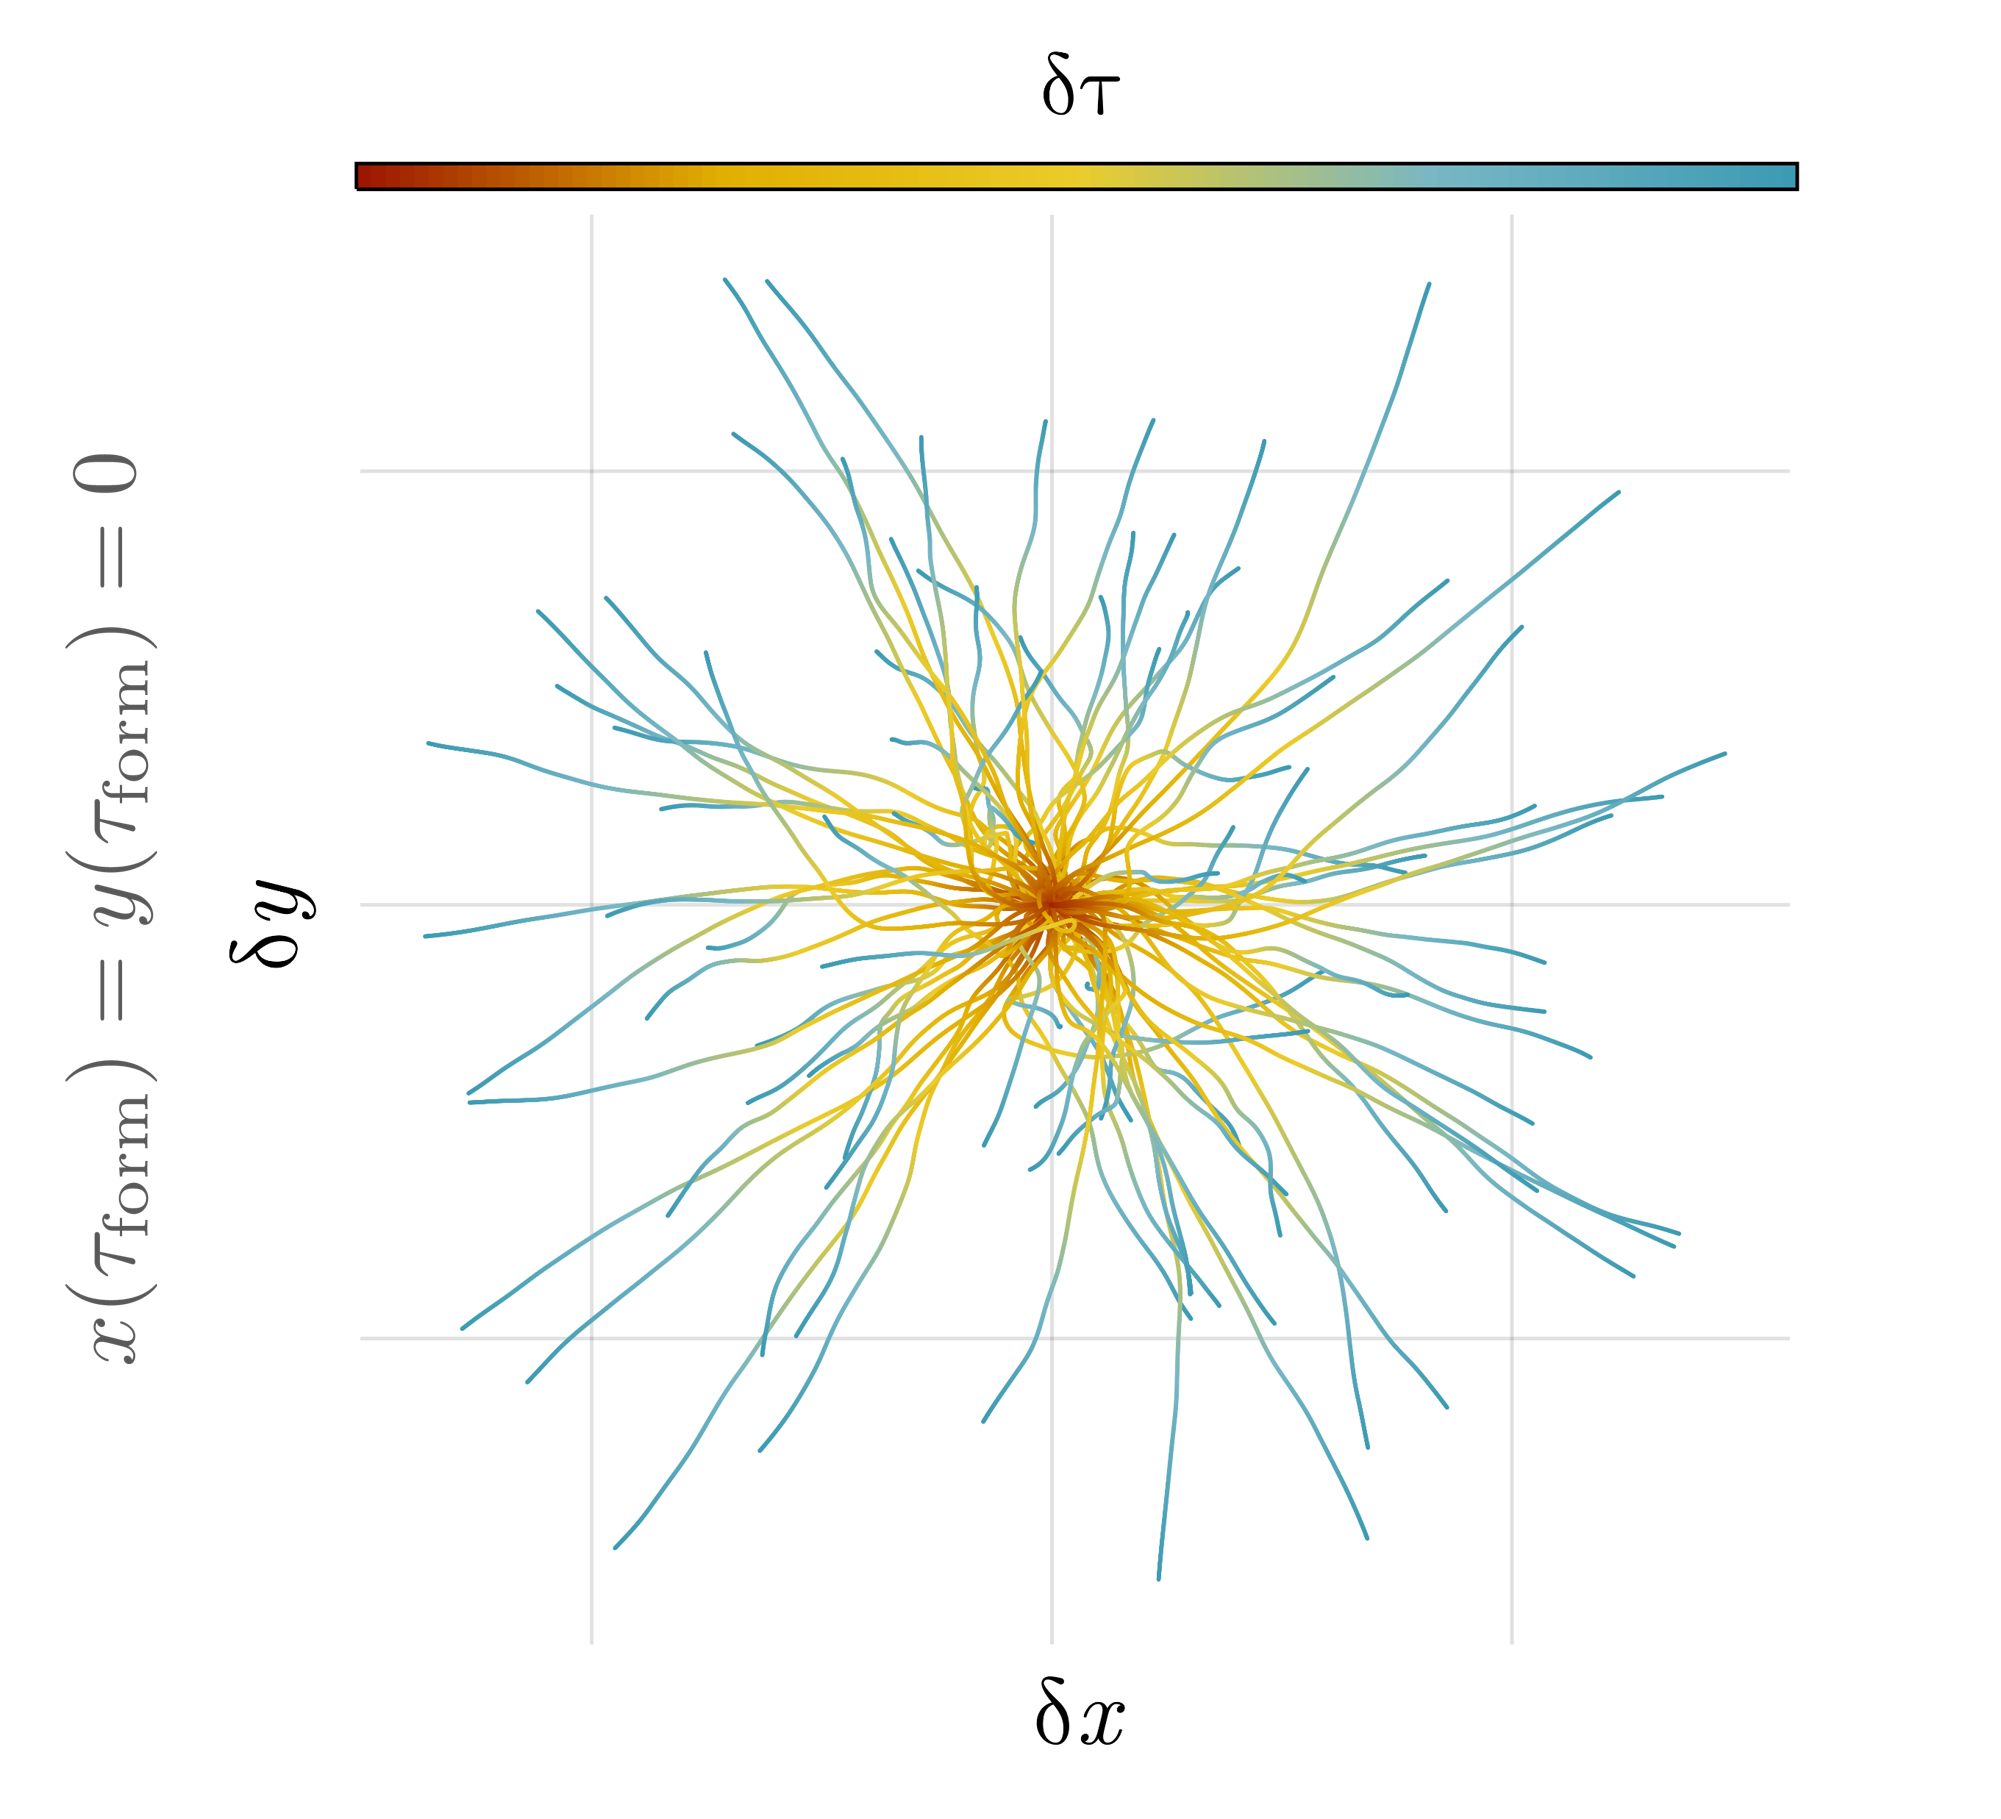
\includegraphics[width=1.1\columnwidth]{images/wong_coord.png}
%                 \end{figure}
%                 \column{.025\textwidth}
%         \column{.3\textwidth}
%             \begin{itemize}
%                 \setbeamertemplate{itemize item}{\raisebox{0.2em}{\scalebox{0.7}{${\color{normal}\blacktriangleright}$}}} 
%                 \item \begin{center}\footnotesize {\bfseries Momentum} broadening due to color Lorentz force\end{center}
%             \end{itemize}
%             \vspace{-20pt}
%             \begin{figure}[!hbt]
%                 \centering
%                 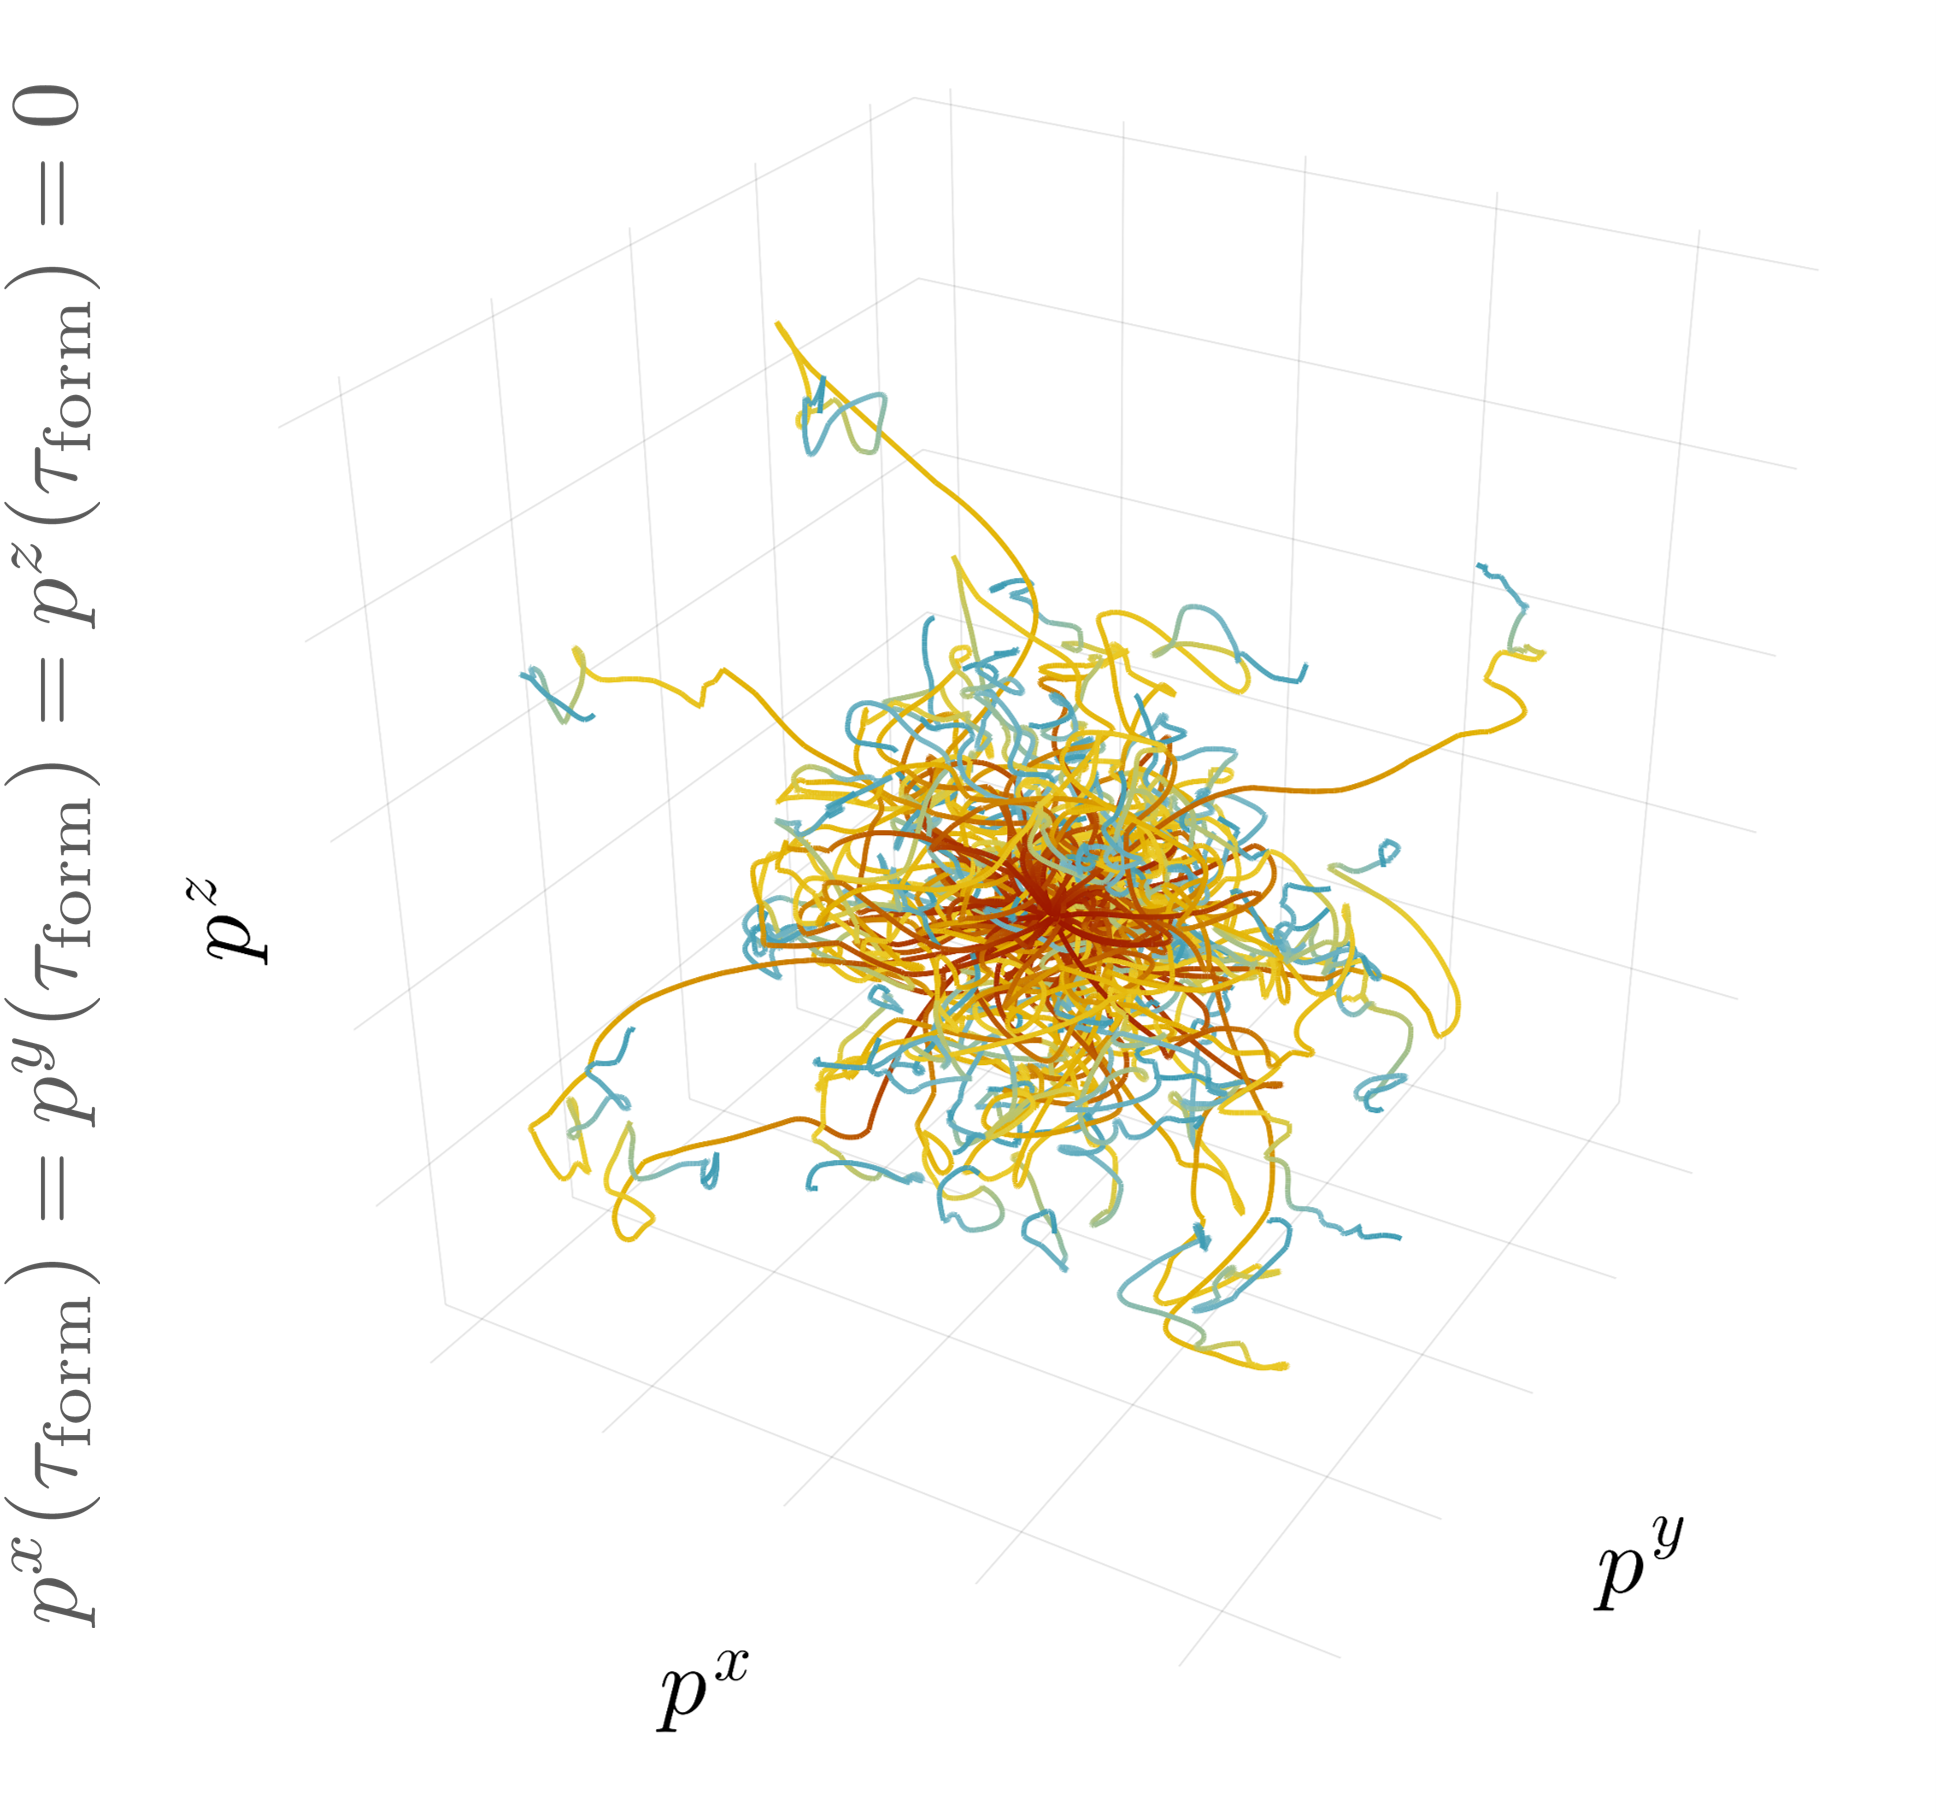
\includegraphics[width=1.1\columnwidth]{images/wong_mom.png}
%             \end{figure}
%             \column{.025\textwidth}
%         \column{.3\textwidth}
%             \begin{itemize}
%                 \setbeamertemplate{itemize item}{\raisebox{0.2em}{\scalebox{0.7}{${\color{normal}\blacktriangleright}$}}} 
%                 \item \begin{center}\footnotesize {\bfseries Color charge} rotation in SU(3) with Wilson lines\end{center}
%             \end{itemize}
%             \vspace{-15pt}
%             \begin{figure}[!hbt]
%                 \centering
%                 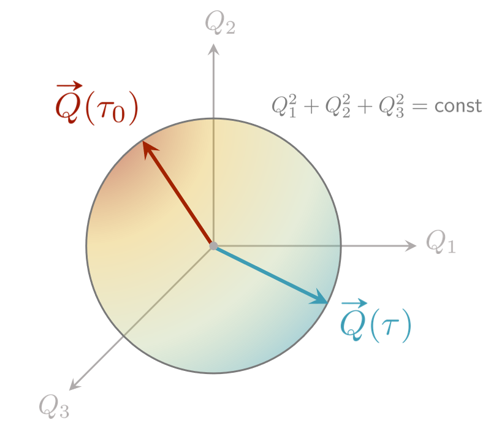
\includegraphics[width=1.05\columnwidth]{images/wong_charge.png}
%             \end{figure}
%             \column{.025\textwidth}
%     \end{columns}

%     \blfootnote{\scriptsize Avramescu, Băran, Greco, Ipp, Müller, Ruggieri  \href{https://arxiv.org/abs/2303.05599}{{\color{palgold}\texttt{[2303.05599]}$^\text{\tiny\faExternalLink}$}}}
% \end{frame}

% %%%%%%%%%%%%%%%%%%%%%%%%%%%%%%%%%%%%%%%%%
% %%%%%%%%%%%%%% SUBSECTION %%%%%%%%%%%%%%%
% %%%%%%%%%%%%%%%%%%%%%%%%%%%%%%%%%%%%%%%%%

% \subsection{Transport coefficients}

% %%%%%%%%%%%%%%%%%%%%%%%%%%%%%%%%%%%%%%%%%
% %%%%%%%%%%%%%%%%% SLIDE %%%%%%%%%%%%%%%%%
% %%%%%%%%%%%%%%%%%%%%%%%%%%%%%%%%%%%%%%%%%

% \begin{frame}
%     \frametitle{Transport coefficient $\kappa$}
%     % \framesubtitle{Momentum broadening in glasma}
%     % \vspace{-10pt}
%     \begin{columns}[onlytextwidth,t]
%         \column{.033\textwidth}
%         \column{.5\textwidth}

%         \begin{figure}
%             \centering
%             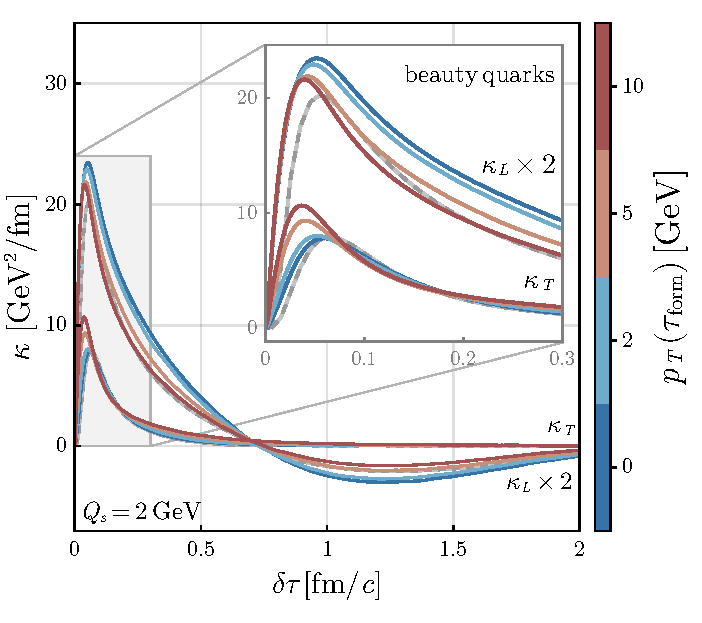
\includegraphics[width=0.9\textwidth]{images/hp23_mom_broad_kappa_anis_wong_vs_kappa-cropped.pdf}
%         \end{figure}
%        \column{.033\textwidth}
%        \column{.4\textwidth}
%         \begin{custombox}{Classical transport}{lightgray}
%             \small
%             \begin{varwidth}{0.95\textwidth}
%             \begin{itemize}
%                 \setbeamertemplate{itemize item}{\raisebox{0.2em}{\scalebox{0.7}{${\color{palteal}\blacktriangleright}$}}} 
%                 \item {\color{palteal}\bfseries Momentum broadening}\\ ${\color{palteal}\boldsymbol{\delta p^2_i}}(\tau)=p^2_i(\tau)-p^2_i(\tau_\mathrm{form})$
%                 \setbeamertemplate{itemize item}{\raisebox{0.2em}{\scalebox{0.7}{${\color{palgold}\blacktriangleright}$}}} 
%                 \item {\color{palgold}\bfseries Transport coefficient}\\ ${\color{palgold}\boldsymbol{\kappa_i}}(\tau)=\dfrac{\mathrm{d}}{\mathrm{d}\tau}\langle{\color{palteal}\boldsymbol{\delta p^2_i}}(\tau)\rangle$ 
%                 \\[5pt]
%                 {\scriptsize\color{lightgray} Formation time $\tau_\mathrm{form}$\\
%                 Longitudinal $i=L$, transverse $i=T$}
%             \end{itemize}
%             \end{varwidth}
%         \end{custombox}

%         \begin{itemize}
%             \footnotesize
%             \setbeamertemplate{itemize item}{\raisebox{0.2em}{\scalebox{0.7}{${\color{lightgray}\blacktriangleright}$}}}
%             {\color{lightgray}\item {\bfseries Anisotropic} $\kappa_L\neq\kappa_T$
%             \item Rapid increase in $\kappa$ at early times 
%             \item Negative $\kappa_L$ at late times}
%             \setbeamertemplate{itemize item}{\raisebox{0.2em}{\scalebox{0.7}{${\color{palviolet}\blacktriangleright}$}}} 
%             \item {\bfseries\color{palviolet}Large $\boldsymbol{\kappa}$ peak in glasma}
%         \end{itemize}    
              
%         \column{.033\textwidth}
%     \end{columns}
%     \blfootnote{\scriptsize Avramescu, Băran, Greco, Ipp, Müller, Ruggieri  \href{https://arxiv.org/abs/2307.07999}{{\color{palgold}\texttt{[2307.07999]}$^\text{\tiny\faExternalLink}$}}}
% \end{frame}

% %%%%%%%%%%%%%%%%%%%%%%%%%%%%%%%%%%%%%%%%%
% %%%%%%%%%%%%%%%%% SLIDE %%%%%%%%%%%%%%%%%
% %%%%%%%%%%%%%%%%%%%%%%%%%%%%%%%%%%%%%%%%%

% \begin{frame}[noframenumbering]
%     \frametitle{Transport coefficient $\kappa$}
%     % \framesubtitle{Momentum broadening in glasma}
%     % \vspace{-10pt}
%     \begin{columns}[onlytextwidth,t]
%         \column{.033\textwidth}
%         \column{.5\textwidth}

%         \begin{figure}
%             \centering
%             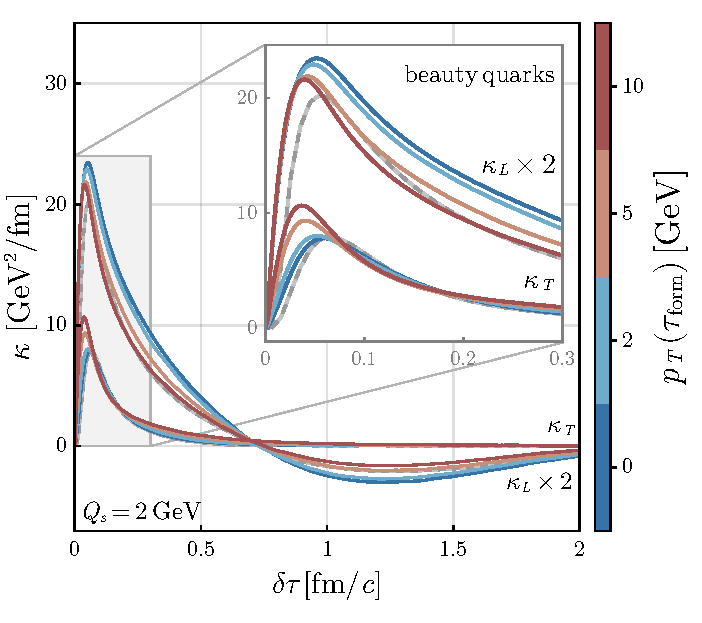
\includegraphics[width=0.9\textwidth]{images/hp23_mom_broad_kappa_anis_wong_vs_kappa-cropped.pdf}
%         \end{figure}
%        \column{.033\textwidth}
%        \column{.4\textwidth}
%         \begin{custombox}{Classical transport}{lightgray}
%             \small
%             \begin{varwidth}{0.95\textwidth}
%             \begin{itemize}
%                 \setbeamertemplate{itemize item}{\raisebox{0.2em}{\scalebox{0.7}{${\color{palteal}\blacktriangleright}$}}} 
%                 \item {\color{palteal}\bfseries Momentum broadening}\\ ${\color{palteal}\boldsymbol{\delta p^2_i}}(\tau)=p^2_i(\tau)-p^2_i(\tau_\mathrm{form})$
%                 \setbeamertemplate{itemize item}{\raisebox{0.2em}{\scalebox{0.7}{${\color{palgold}\blacktriangleright}$}}} 
%                 \item {\color{palgold}\bfseries Transport coefficient}\\ ${\color{palgold}\boldsymbol{\kappa_i}}(\tau)=\dfrac{\mathrm{d}}{\mathrm{d}\tau}\langle{\color{palteal}\boldsymbol{\delta p^2_i}}(\tau)\rangle$ 
%                 \\[5pt]
%                 {\scriptsize\color{lightgray} Formation time $\tau_\mathrm{form}$\\
%                 Longitudinal $i=L$, transverse $i=T$}
%             \end{itemize}
%             \end{varwidth}
%         \end{custombox}

%         \begin{custombox}{Limitation}{palviolet}
%             \small
%             \begin{varwidth}{0.75\textwidth}
%             \begin{itemize}
%                 \setbeamertemplate{itemize item}{\raisebox{0.2em}{\scalebox{0.7}{${\color{palviolet}\blacktriangleright}$}}} 
%                 \item Transport coefficients $\neq$ {\color{palviolet}\bfseries measurable} quantities
%             \end{itemize}
%             \end{varwidth}
%         \end{custombox} 
              
%         \column{.033\textwidth}
%     \end{columns}
%     \blfootnote{\scriptsize Avramescu, Băran, Greco, Ipp, Müller, Ruggieri  \href{https://arxiv.org/abs/2307.07999}{{\color{palgold}\texttt{[2307.07999]}$^\text{\tiny\faExternalLink}$}}}
% \end{frame}

%%%%%%%%%%%%%%%%%%%%%%%%%%%%%%%%%%%%%%%%%
%%%%%%%%%%%%%%%% SECTION %%%%%%%%%%%%%%%%
%%%%%%%%%%%%%%%%%%%%%%%%%%%%%%%%%%%%%%%%%

\section{Phenomenology implications}

\setbeamertemplate{background}{
\tikz[overlay,remember picture] \node[opacity=0.15, at=(current page.center)] {
   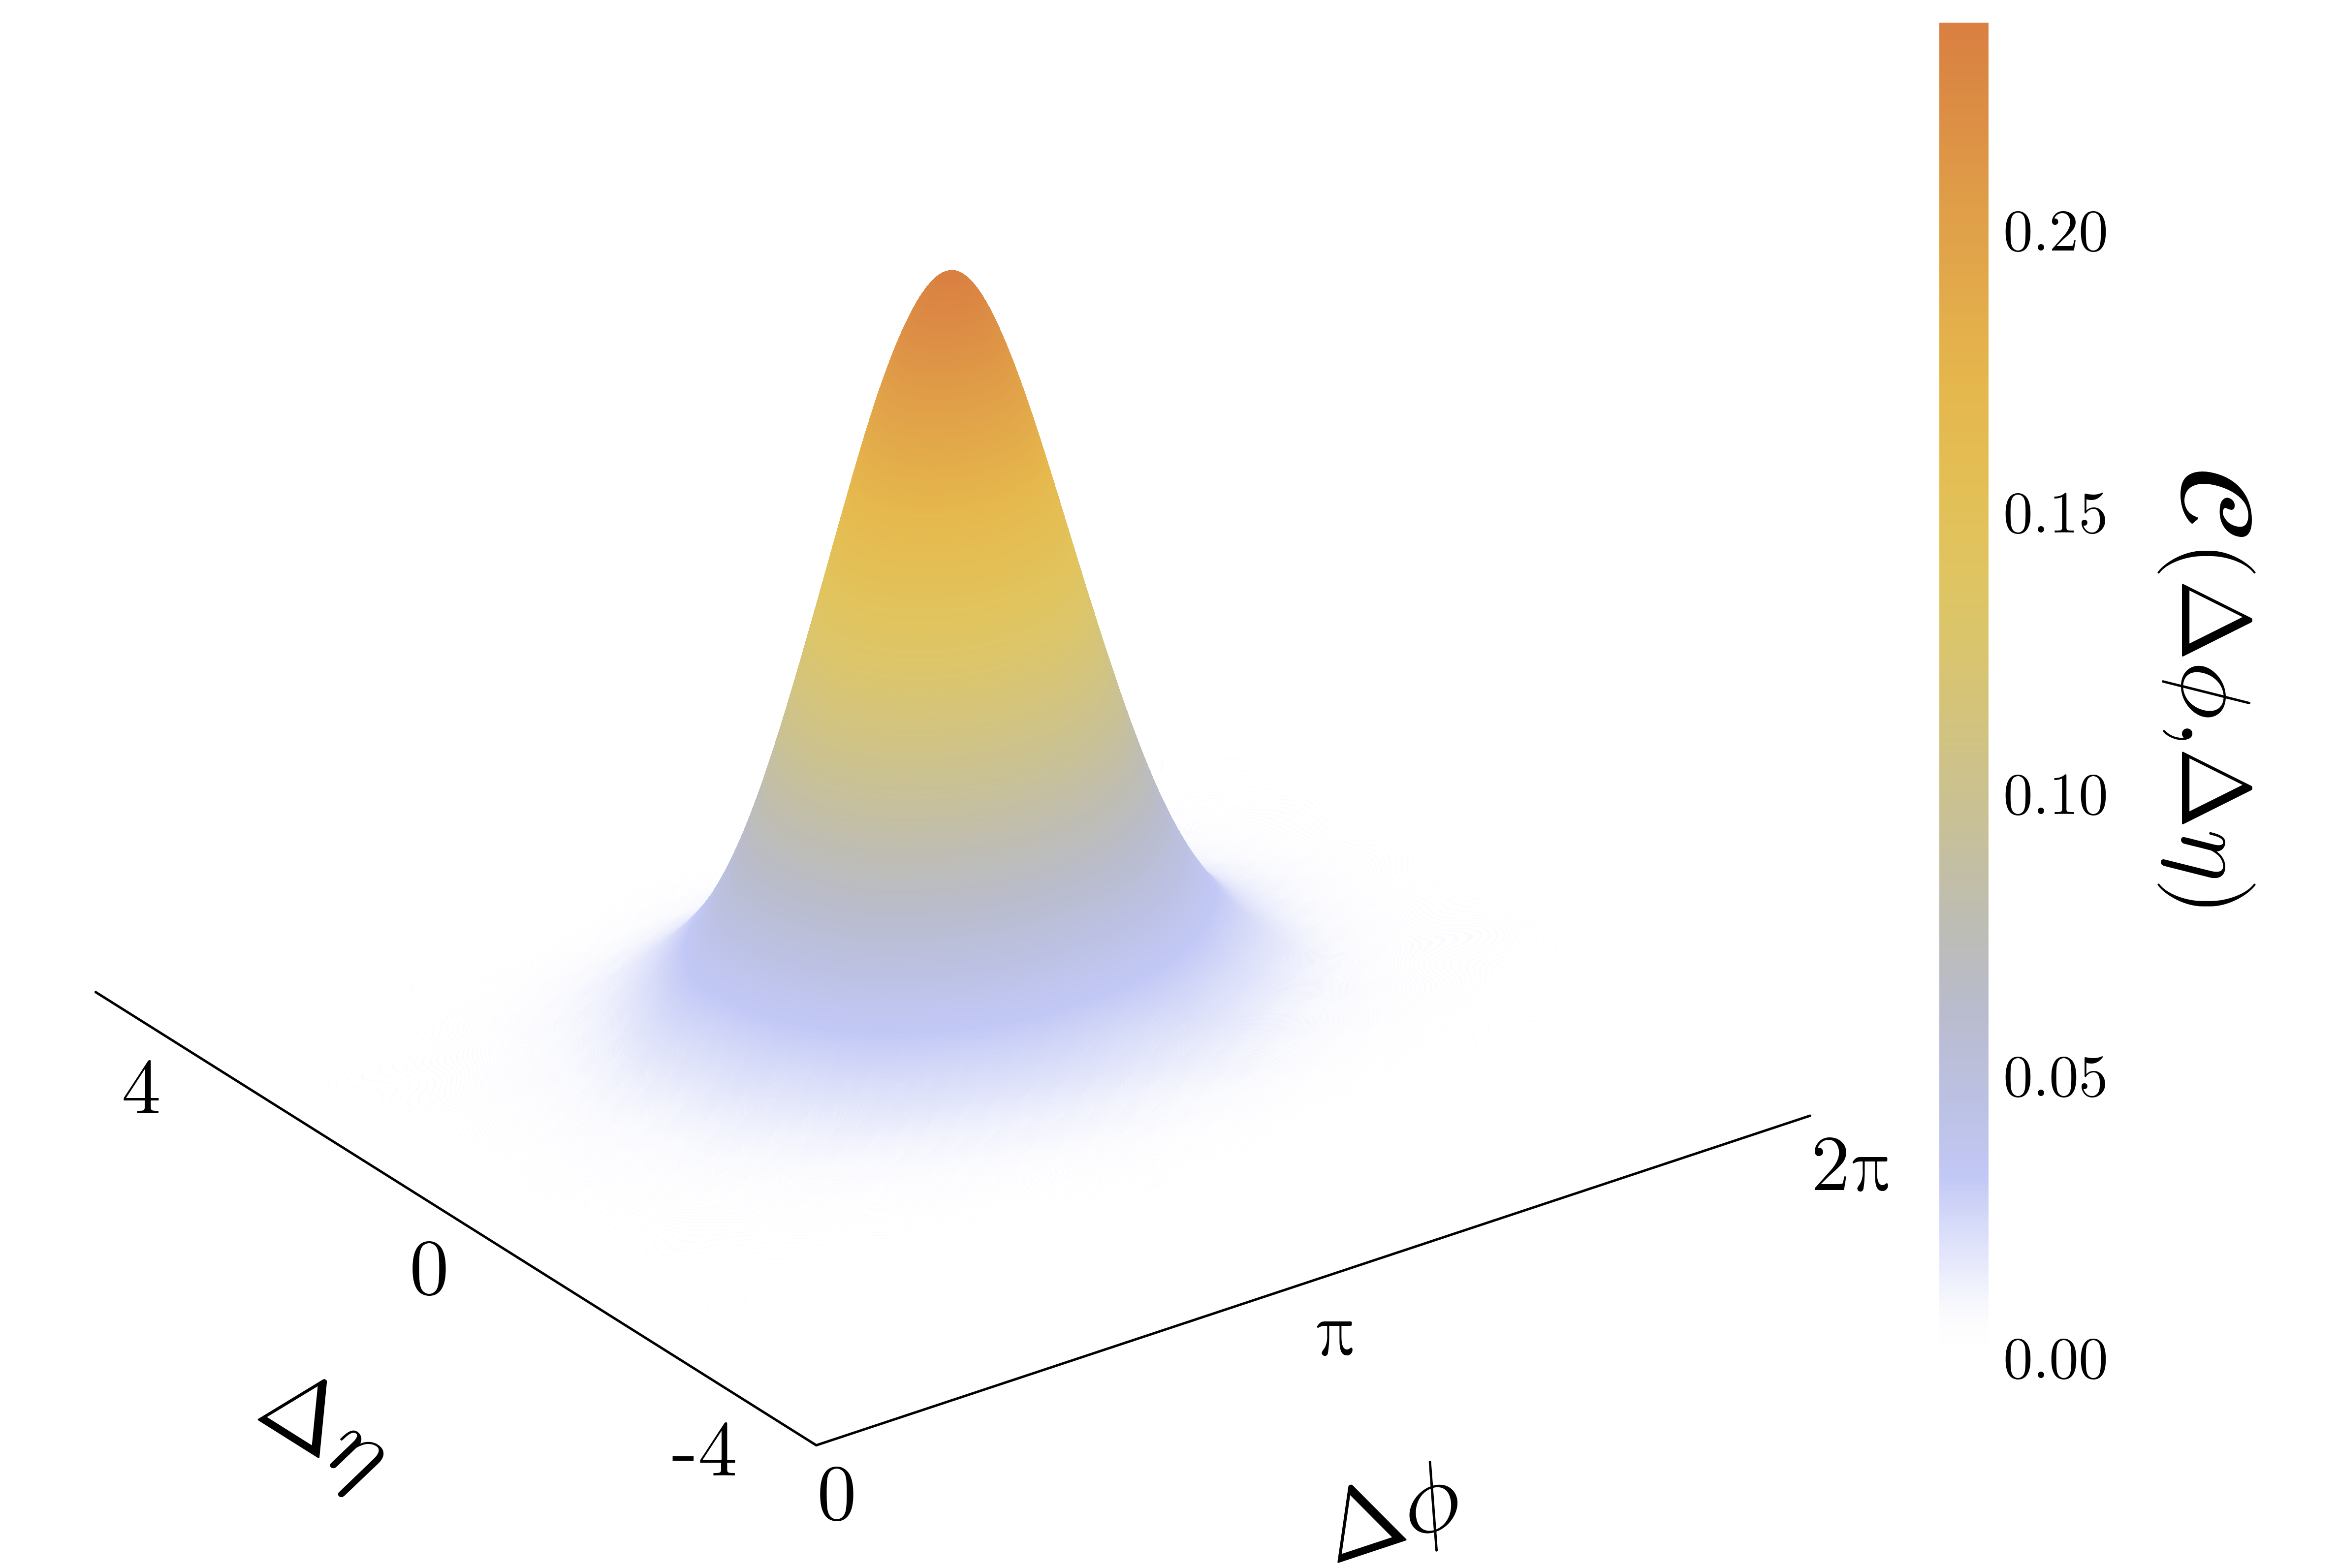
\includegraphics[height=0.8\paperheight]{images/Cdetadphi_3D_toy_charm_pT_1_tau_0.1_crop.png}};
}
\begin{frame}[plain,noframenumbering]{}
    \begin{center}
        \vspace{1cm}
        {\large\color{normal}How to probe pre-equilibrium}\\[0.3cm]
        {\huge\color{destacado}Phenomenology implications}\\[0.3cm]
    \end{center}
\end{frame}
\setbeamertemplate{background}{}

%%%%%%%%%%%%%%%%%%%%%%%%%%%%%%%%%%%%%%%%%
%%%%%%%%%%%%%% SUBSECTION %%%%%%%%%%%%%%%
%%%%%%%%%%%%%%%%%%%%%%%%%%%%%%%%%%%%%%%%%

\subsection{Nuclear modification factor}

%%%%%%%%%%%%%%%%%%%%%%%%%%%%%%%%%%%%%%%%%
%%%%%%%%%%%%%%%%% SLIDE %%%%%%%%%%%%%%%%%
%%%%%%%%%%%%%%%%%%%%%%%%%%%%%%%%%%%%%%%%%

\begin{frame}
    \frametitle{Effect of glasma on spectra}
    % \framesubtitle{Procedure to extract $R_{AA}$}
    \vspace{-10pt}
    \begin{columns}[onlytextwidth,t]
        \column{.033\textwidth}
        \column{.45\textwidth}
        \begin{center}
            \begin{custombox}{{\normalsize Effect of glasma}}{raapink}
                \small
                \begin{varwidth}{0.85\textwidth}
                \begin{itemize}
                    \itemsep0em 
                    \setbeamertemplate{itemize item}{\raisebox{0.2em}{\scalebox{0.7}{${\color{raapink}\blacktriangleright}$}}} 
                    \footnotesize
                    \item Initial flat $p_T$ distribution
                    \item $p_T$ migration from small to large $p_T$
                \end{itemize}
                \end{varwidth}
            \end{custombox}

            \vspace{-15pt}
            \begin{figure}
                \centering
                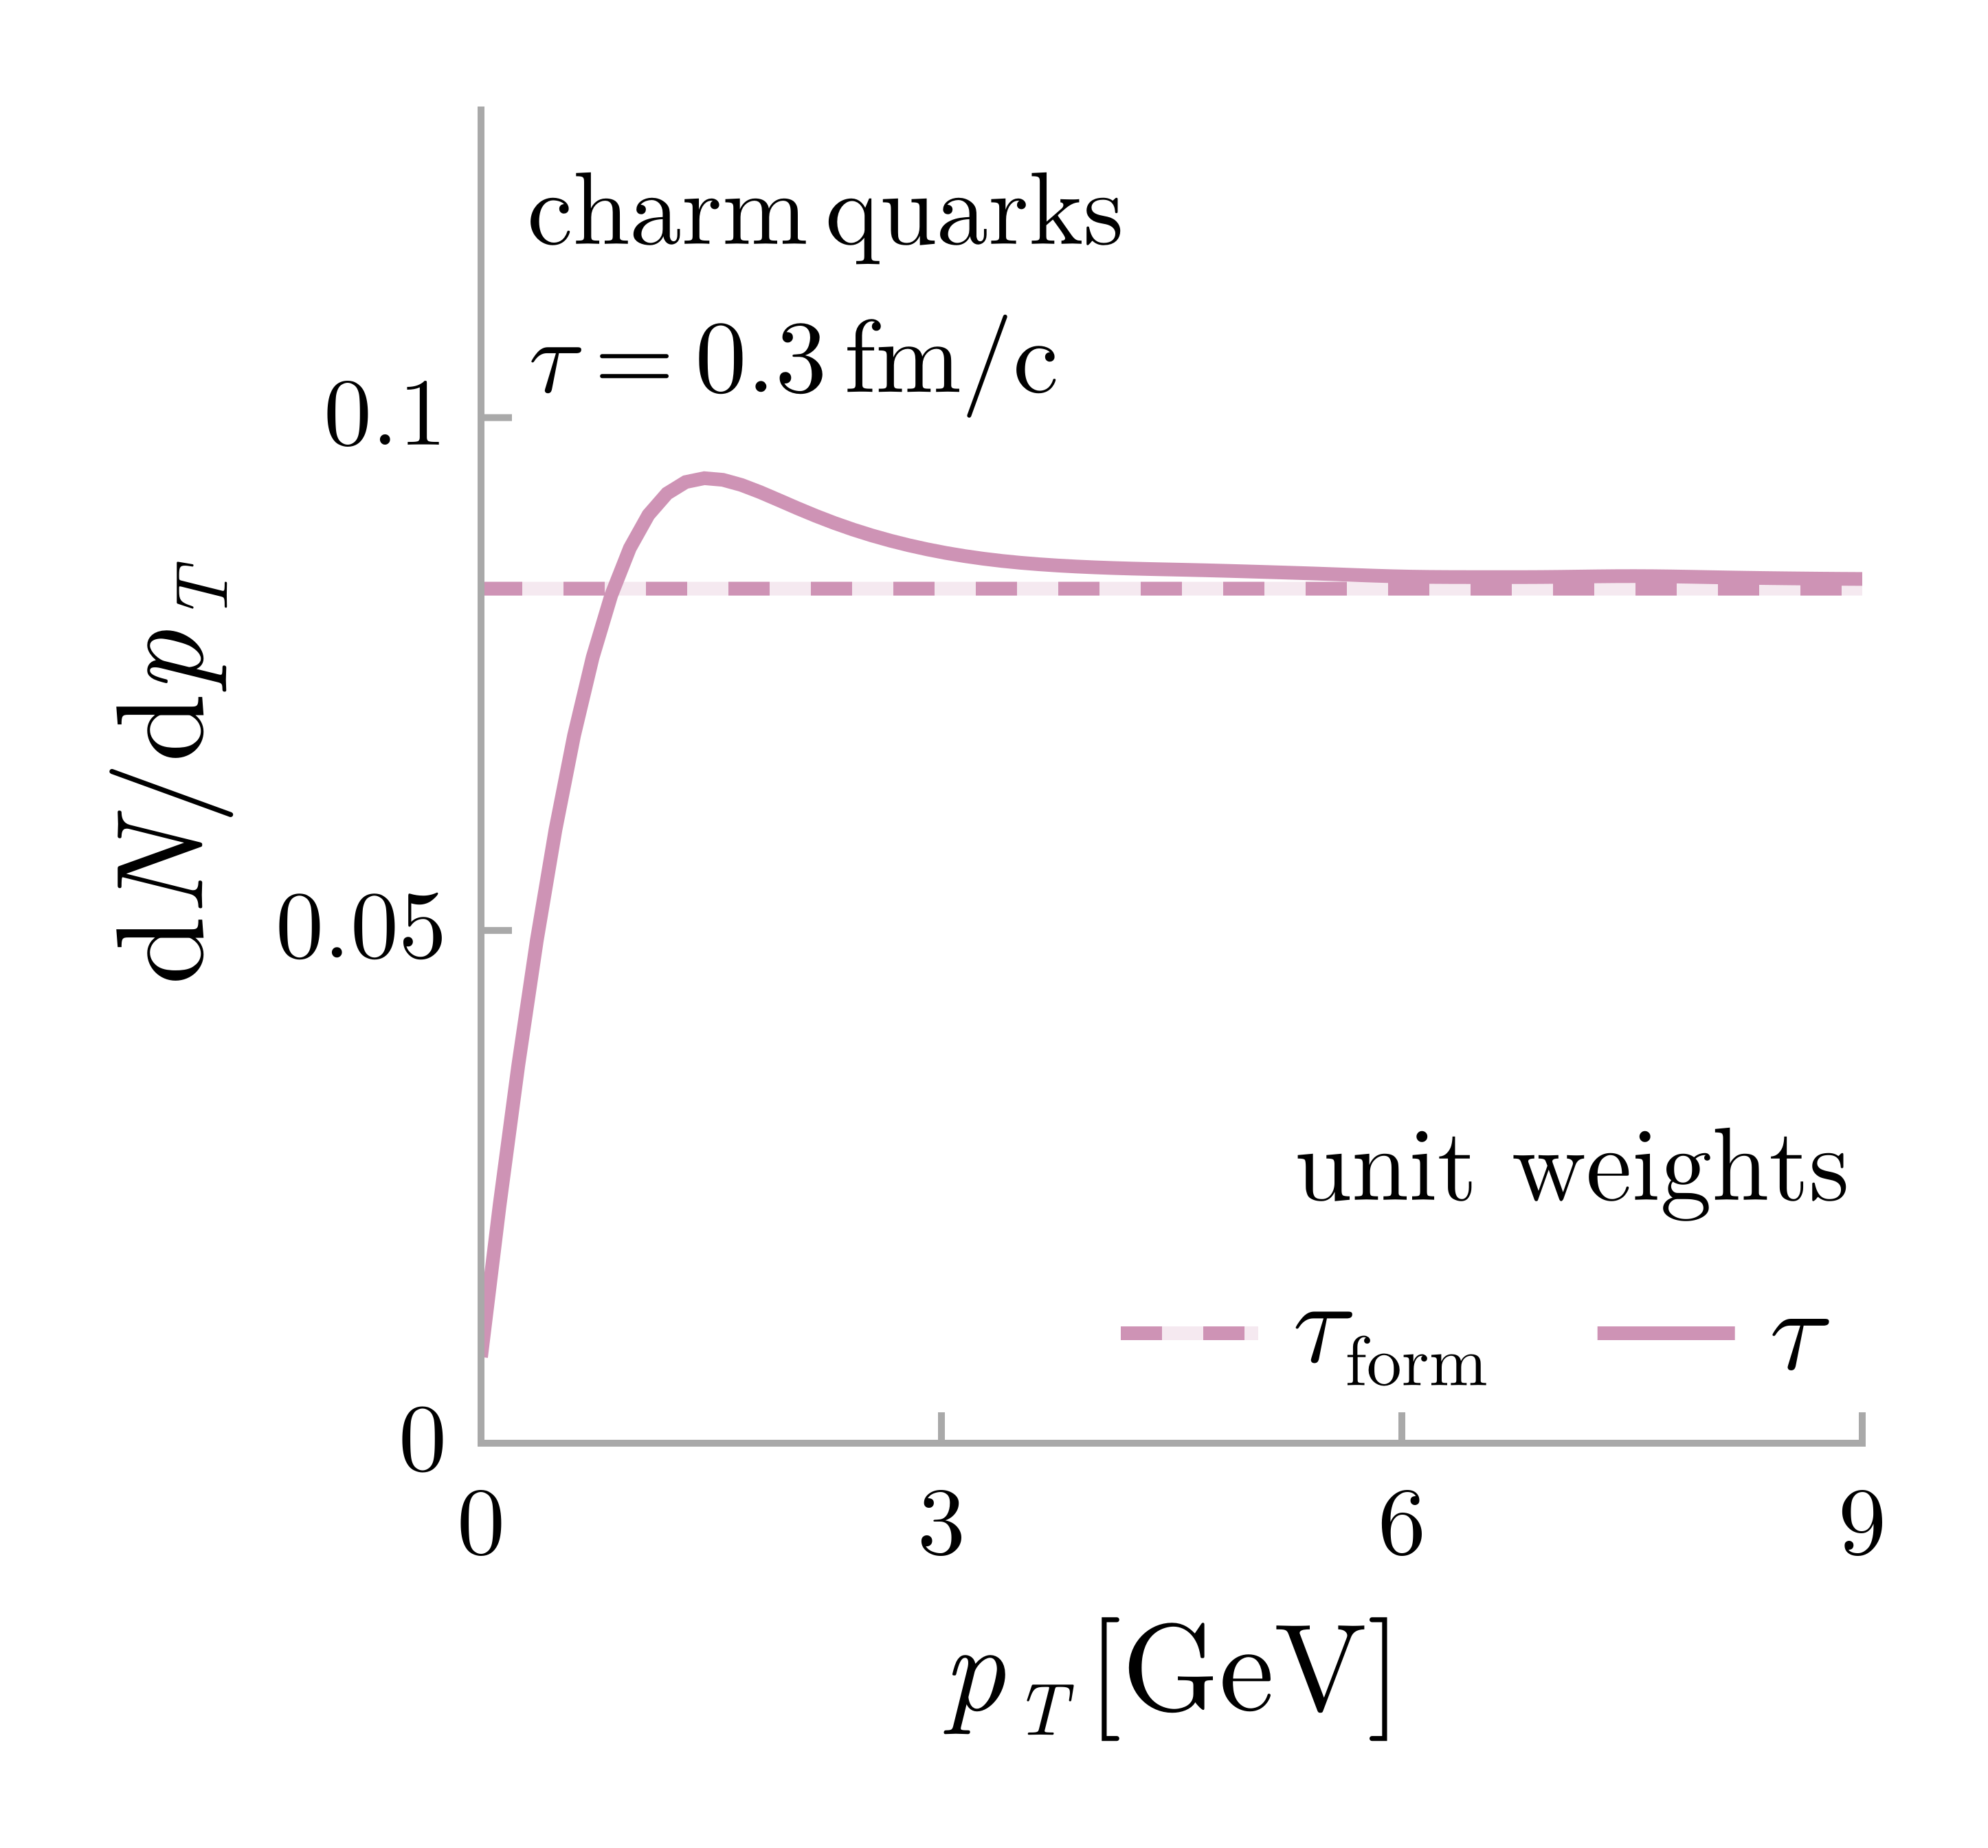
\includegraphics[height=0.63\textheight]{images/final_sketch_raa_gl_fonll_v4_gl.png}
            \end{figure}
        \end{center}
        

       \column{.033\textwidth}
       \column{.45\textwidth}
       \begin{center}
        \begin{custombox}{{\normalsize Effect of initial spectrum}}{raablue}
            \small
            \begin{varwidth}{0.9\textwidth}
            \begin{itemize}
                \itemsep0em
                \setbeamertemplate{itemize item}{\raisebox{0.2em}{\scalebox{0.7}{${\color{raablue}\blacktriangleright}$}}} 
                \footnotesize
                \item Initial pQCD FONLL $p_T$ spectrum\\
                {\scriptsize\color{lightgray}Fixed-Order+Next-to-Leading Logarithm}
            \end{itemize}
            \end{varwidth}
        \end{custombox}

        \vspace{-13pt}
        \begin{figure}
            \centering
            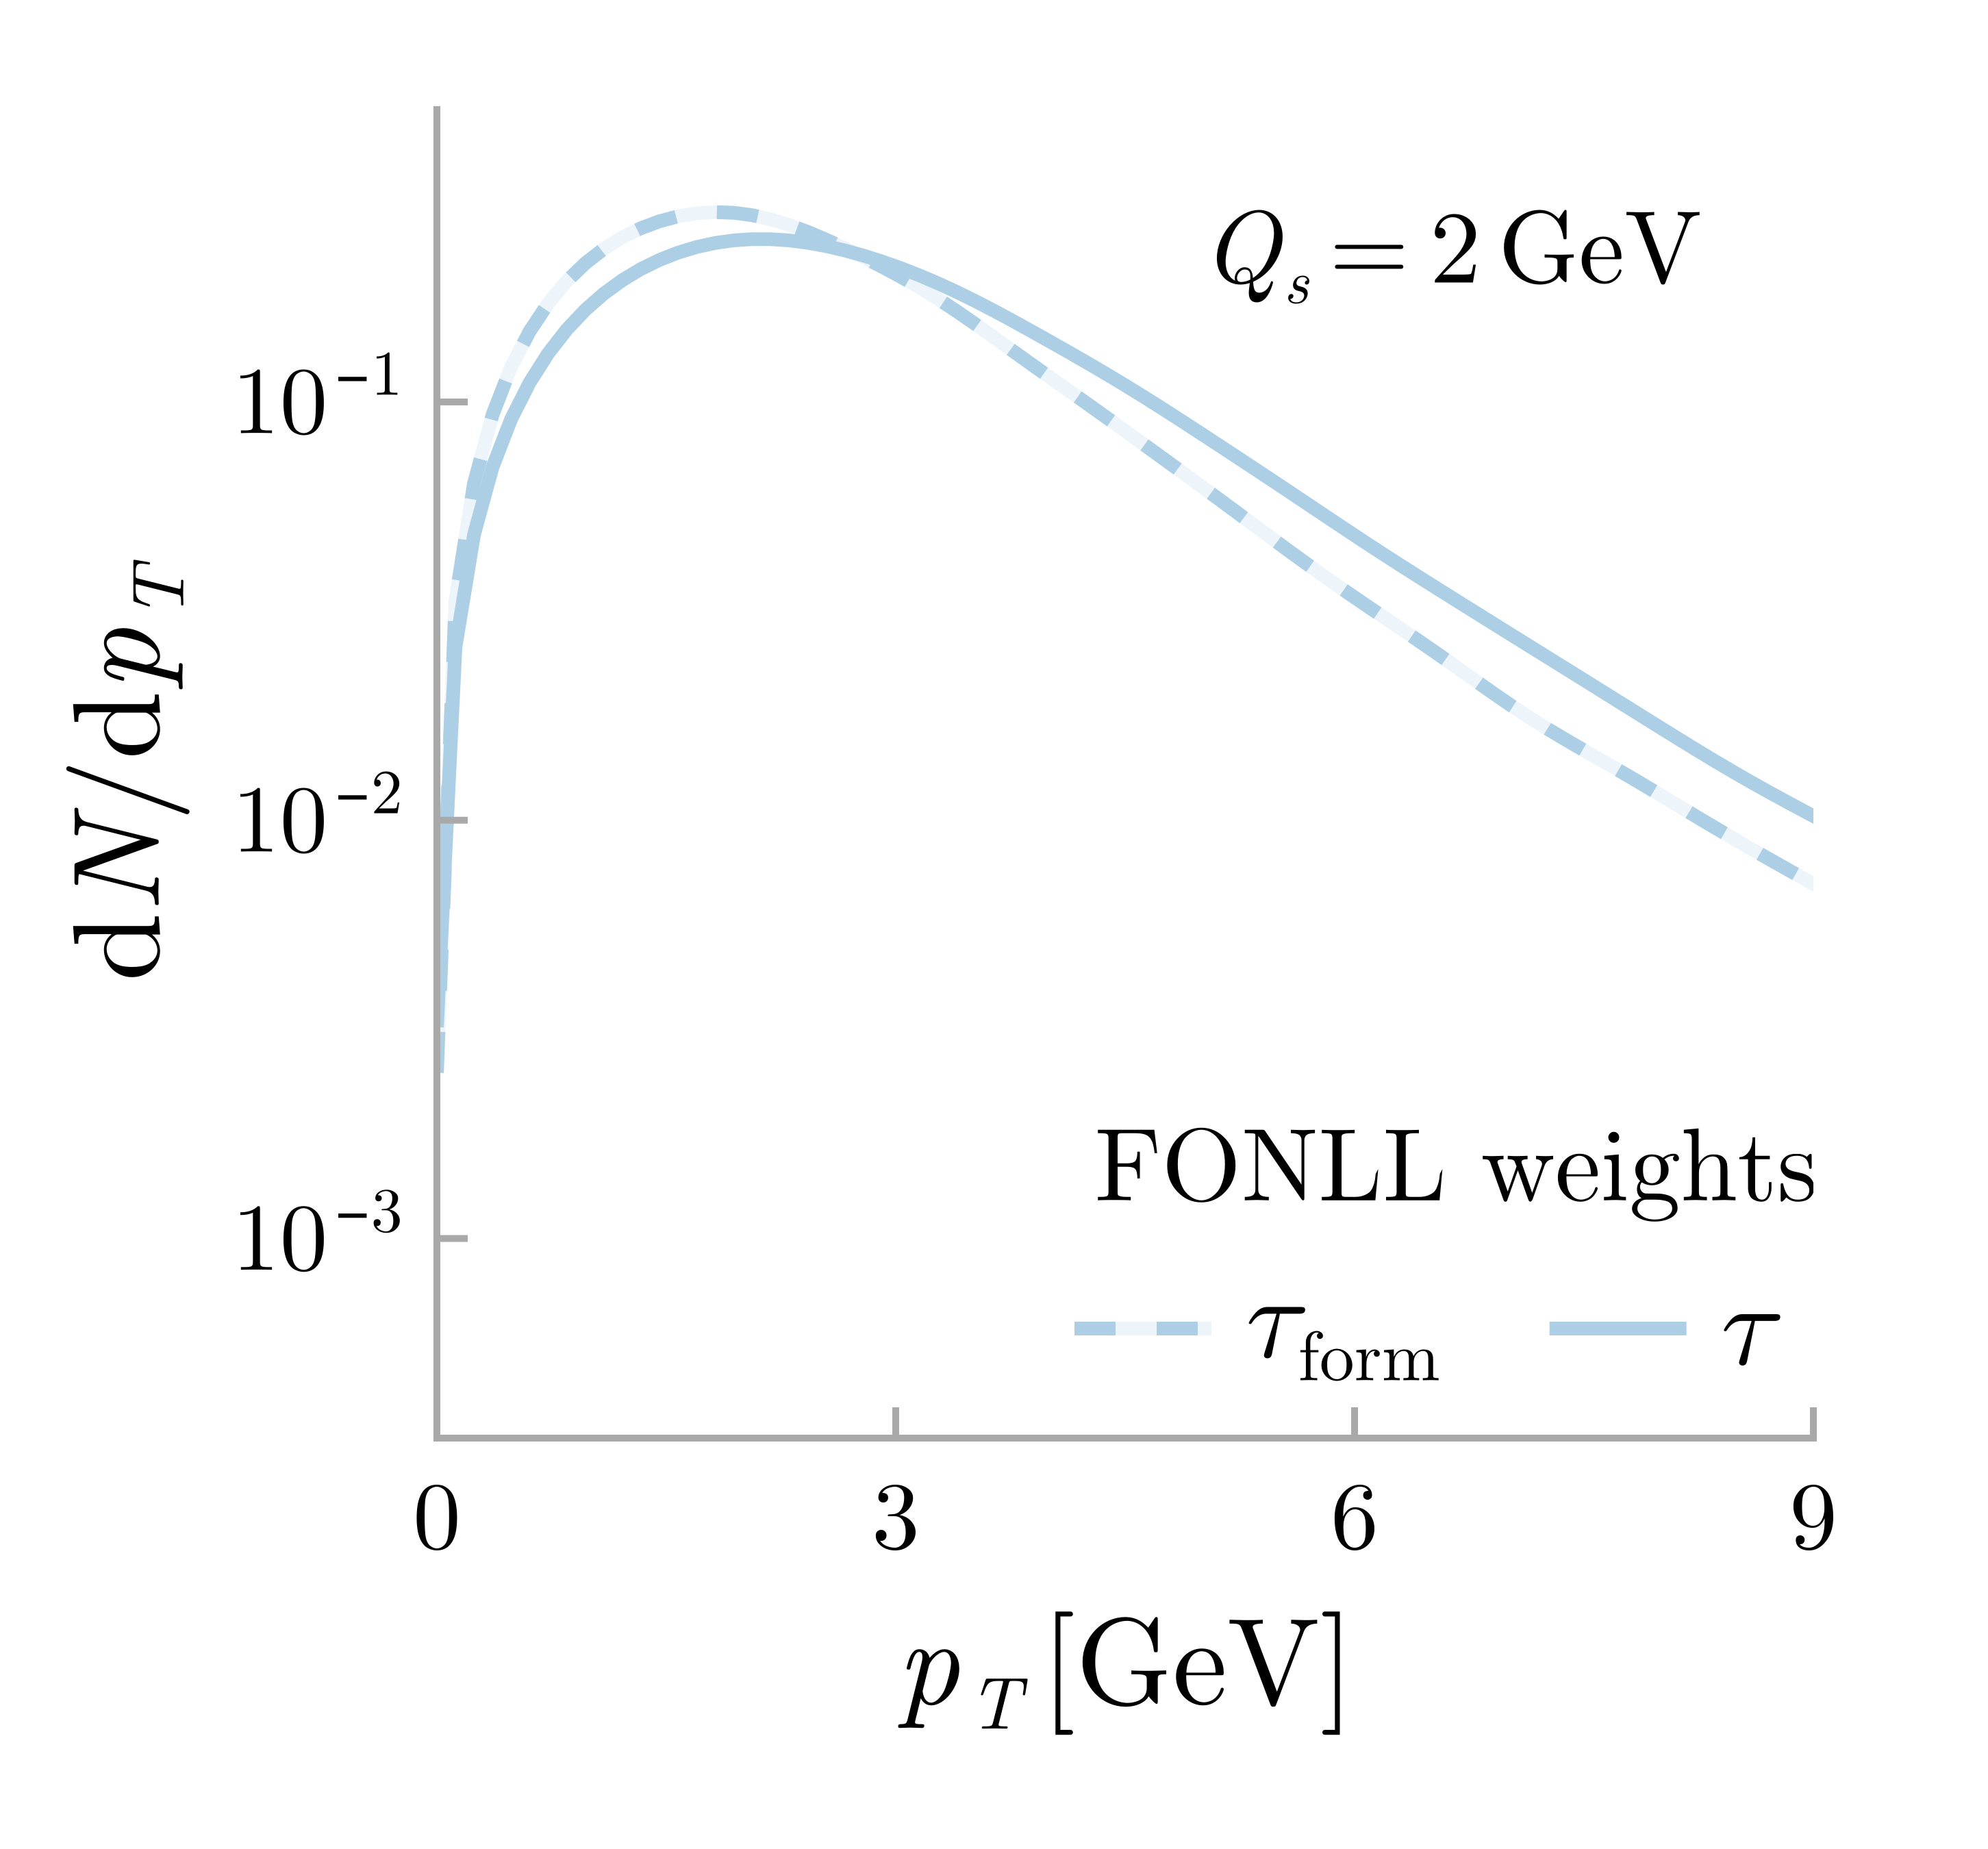
\includegraphics[height=0.63\textheight]{images/final_sketch_raa_gl_fonll_v4_fonll.png}
        \end{figure}

       \end{center}
        \column{.033\textwidth}
    \end{columns}

    \blfootnote{\scriptsize Cacciari, Greco, Nason \href{https://arxiv.org/abs/hep-ph/9803400}{{\color{palgold}\texttt{[hep-ph/9803400]$^\text{\tiny\faExternalLink}$}}}, \href{https://www.lpthe.jussieu.fr/~cacciari/fonll/fonllform.html}{{\color{raablue}\texttt{[FONLL web form]$^\text{\tiny\faLink}$}}}}
\end{frame}

%%%%%%%%%%%%%%%%%%%%%%%%%%%%%%%%%%%%%%%%%
%%%%%%%%%%%%%%%%% SLIDE %%%%%%%%%%%%%%%%%
%%%%%%%%%%%%%%%%%%%%%%%%%%%%%%%%%%%%%%%%%

\begin{frame}
    \frametitle{Nuclear modification factor}
    \framesubtitle{Extraction of $R_{AA}$ in glasma}
    \vspace{-10pt}
    \begin{columns}[onlytextwidth,t]
        \column{.033\textwidth}
        \column{.4\textwidth}
        \begin{center}
    
            \begin{figure}
                \centering
                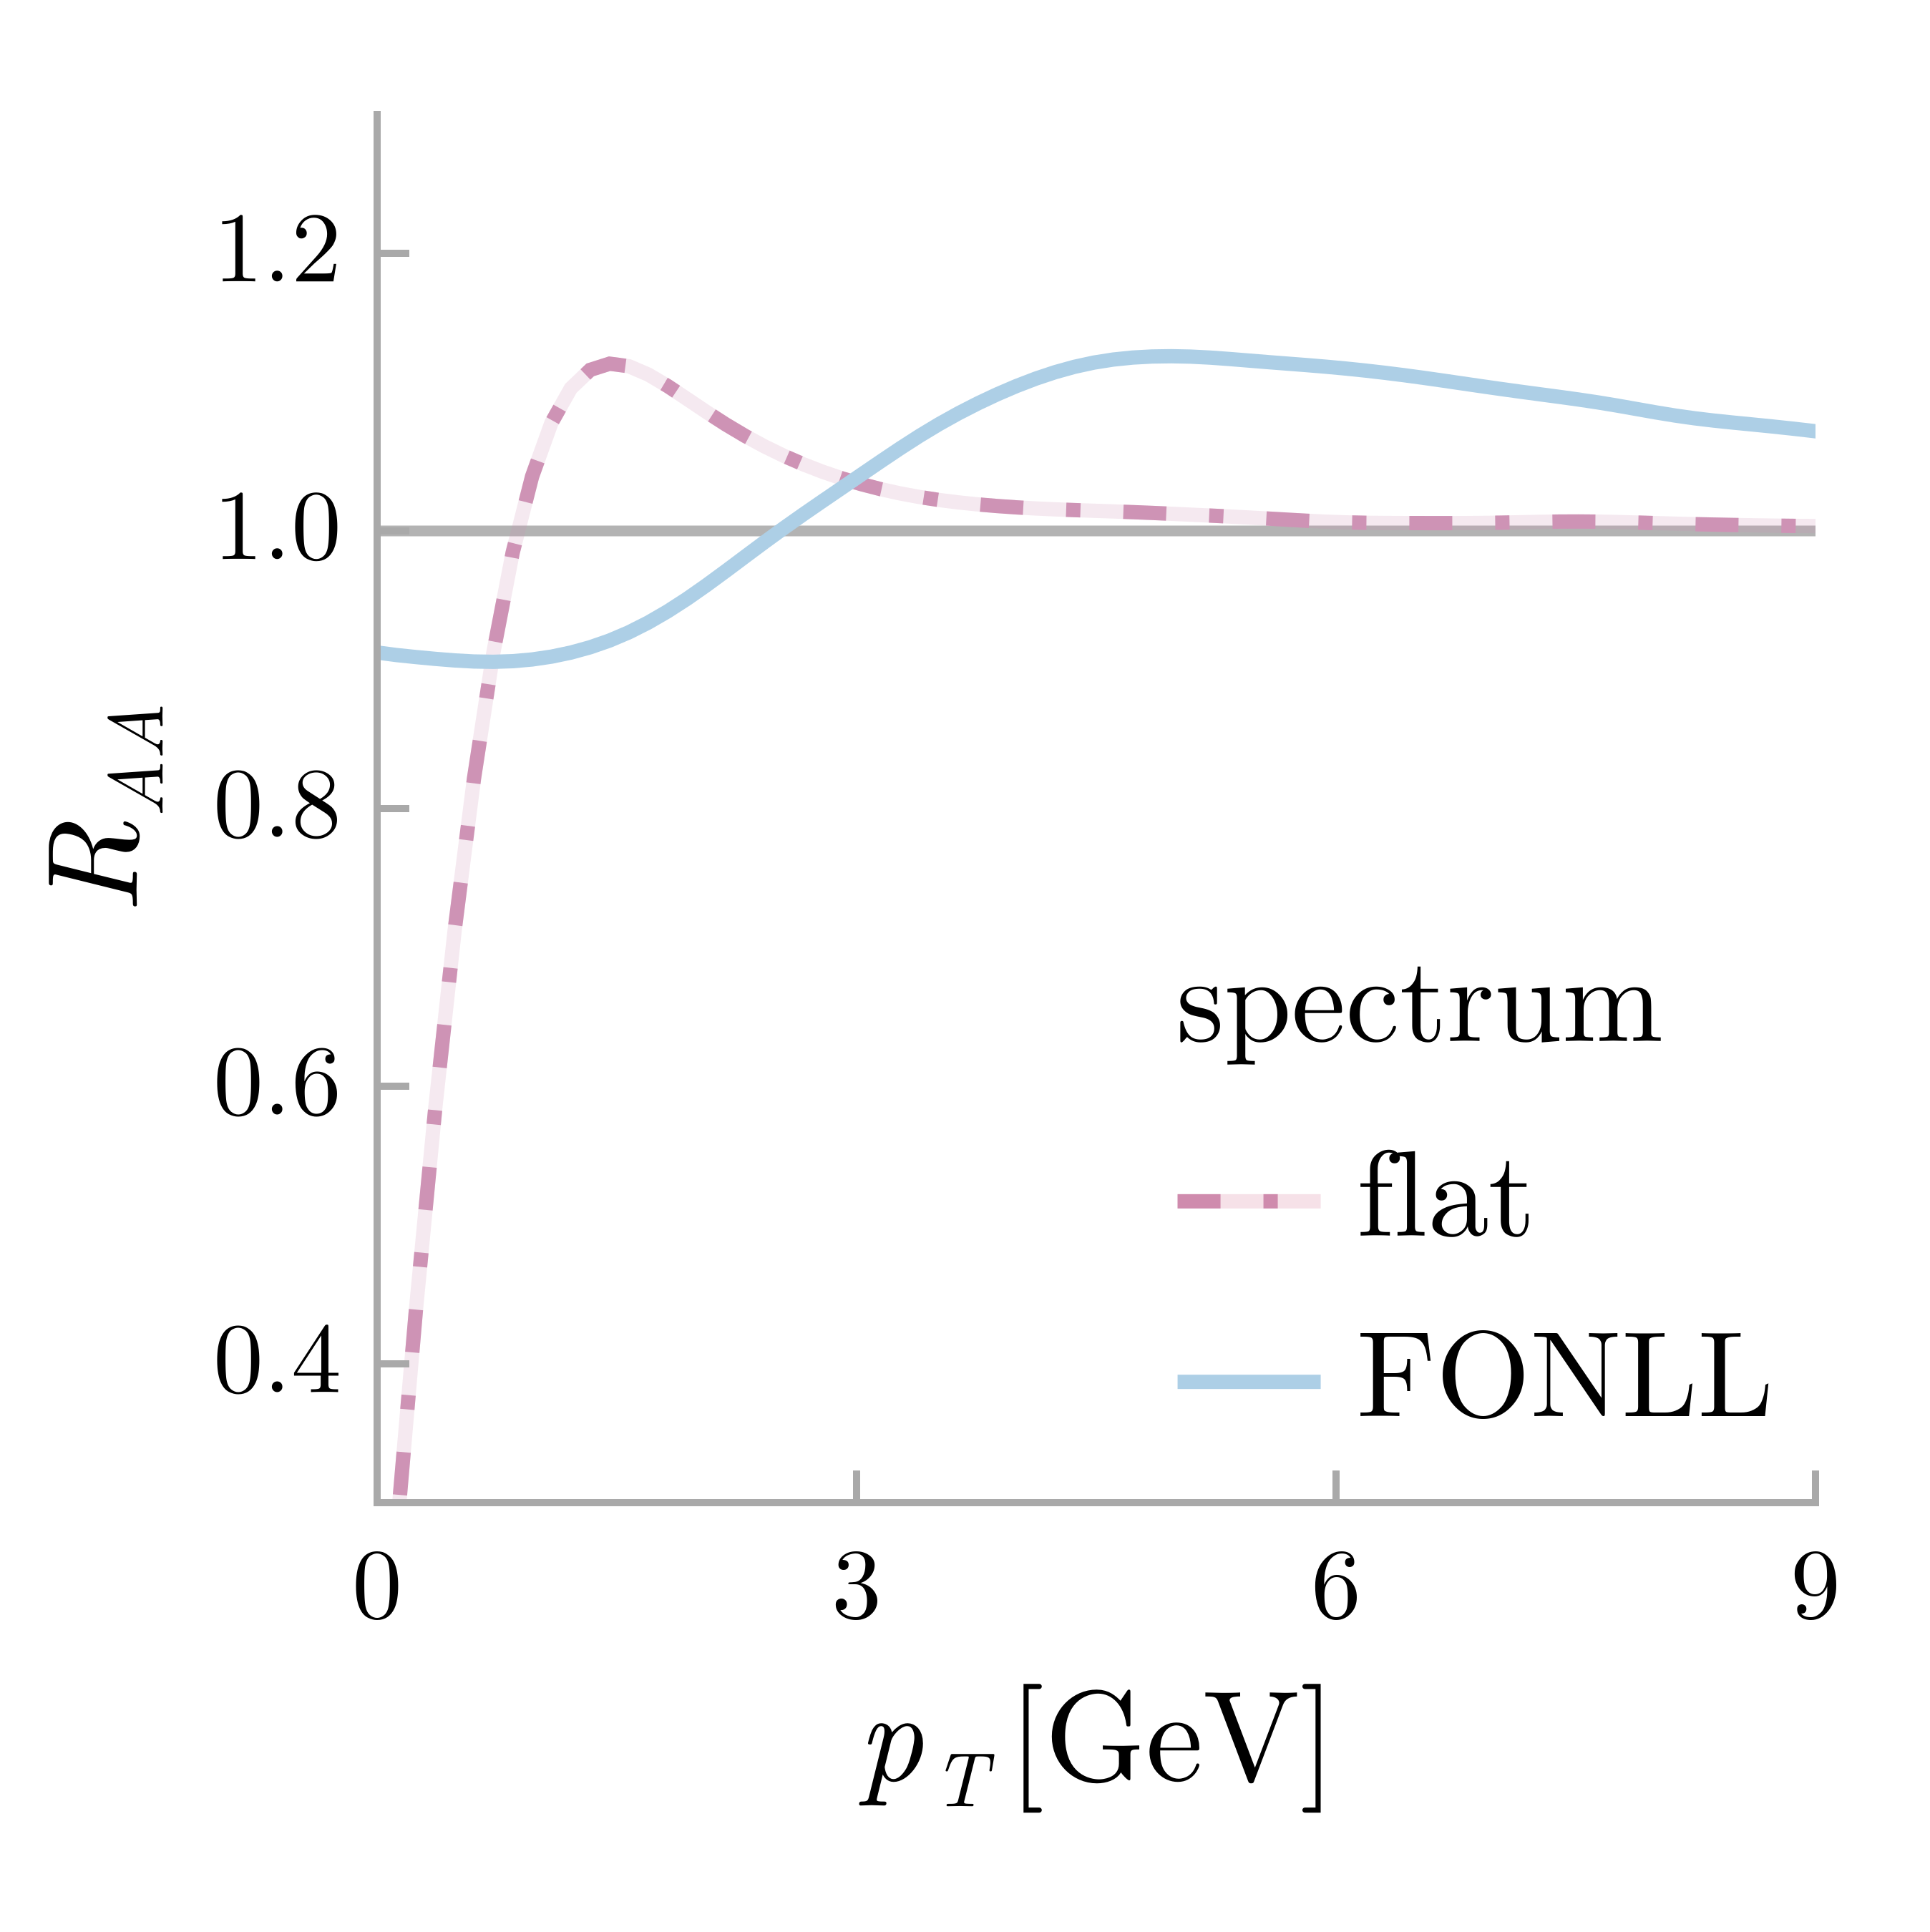
\includegraphics[width=0.95\textwidth]{images/final_sketch_raa_gl_fonll_v4_crop_2.png}
            \end{figure}
        \end{center}
        

       \column{.033\textwidth}
       \column{.5\textwidth}
       \begin{center}
        \begin{custombox}{$\boldsymbol{R_{AA}}$ in glasma}{lightgray}
            \small
            \begin{varwidth}{0.85\textwidth}
            \begin{itemize}
                \itemsep0em
                \setbeamertemplate{itemize item}{\raisebox{0.2em}{\scalebox{0.7}{${\color{lightgray}\blacktriangleright}$}}} 
                \item Ratio of ${\color{palviolet}AA}$ to ${\color{palteal}pp}$ normalized spectra
            \end{itemize}
            \end{varwidth}
        \end{custombox}

        \begin{itemize}
            \itemsep0em
            \footnotesize\color{lightgray}
            \setbeamertemplate{itemize item}{\raisebox{0.2em}{\scalebox{0.7}{${\color{lightgray}\blacktriangleright}$}}} 
            \item ${\color{palviolet}AA}$ evolved in {\color{palviolet}glasma}, ${\color{palteal}pp}$ from {\color{palteal}FONLL} 
            \item Glasma spectrum initialized with FONLL
        \end{itemize}
        \vspace{5pt}

        \renewcommand{\eqnhighlightheight}{\vphantom{\mathcal{D}_\mu}\mathstrut}
        \begin{equation*}
            \hspace{0pt}
            R_{AA}(\tau)=\dfrac{1}{A^2}\dfrac{{\color{palgold}\sigma}^{\textcolor{normal}{AA}}_{\mathrm{\textcolor{palgold}{tot}}}}{\eqnmark[palgold]{sigma}{{\color{palgold}\sigma}^{\textcolor{normal}{pp}}_{\mathrm{\textcolor{palgold}{tot}}}}}\dfrac{\eqnmark[palviolet]{gl}{\mathrm{d}N/\mathrm{d}p_T}(\tau)}{\eqnmark[palteal]{fonll}{\mathrm{d}N^{pp}/\mathrm{d}p_T}}
        \end{equation*}
        \annotate[yshift=-0.5em]{below, left}{sigma}{\tiny total $Q\overline{Q}$ cross section}
        \annotate[yshift=1.2em]{above, left}{gl}{\tiny glasma spectrum}
        \annotate[yshift=-2em]{below, left}{fonll}{\tiny FONLL spectrum}

       \end{center}
        \column{.033\textwidth}
    \end{columns}
\end{frame}


%%%%%%%%%%%%%%%%%%%%%%%%%%%%%%%%%%%%%%%%%
%%%%%%%%%%%%%%%%% SLIDE %%%%%%%%%%%%%%%%%
%%%%%%%%%%%%%%%%%%%%%%%%%%%%%%%%%%%%%%%%%

\begin{frame}
    \frametitle{$R_{AA}$ in glasma}
    % \framesubtitle{Temporal evolution, energy dependence}
    \vspace{-15pt}
    \begin{center}
        \begin{columns}[onlytextwidth,t]
            \column{.02\textwidth}
           \column{.47\textwidth}
           \begin{center}
                \begin{custombox}{\normalsize Time $\boldsymbol{\tau}$ evolution}{palteal}
                    \small
                    \begin{varwidth}{0.88\textwidth}
                    \begin{itemize}
                        \itemsep0em
                        \footnotesize
                        \setbeamertemplate{itemize item}{\raisebox{0.2em}{\scalebox{0.7}{${\color{palteal}\blacktriangleright}$}}} 
                        \item More enhancement in $R_{AA}$ at later $\tau$
                    \end{itemize}
                    \end{varwidth}
                \end{custombox}
            \end{center}
            \vspace{-10pt}
           \begin{figure}
                \centering
                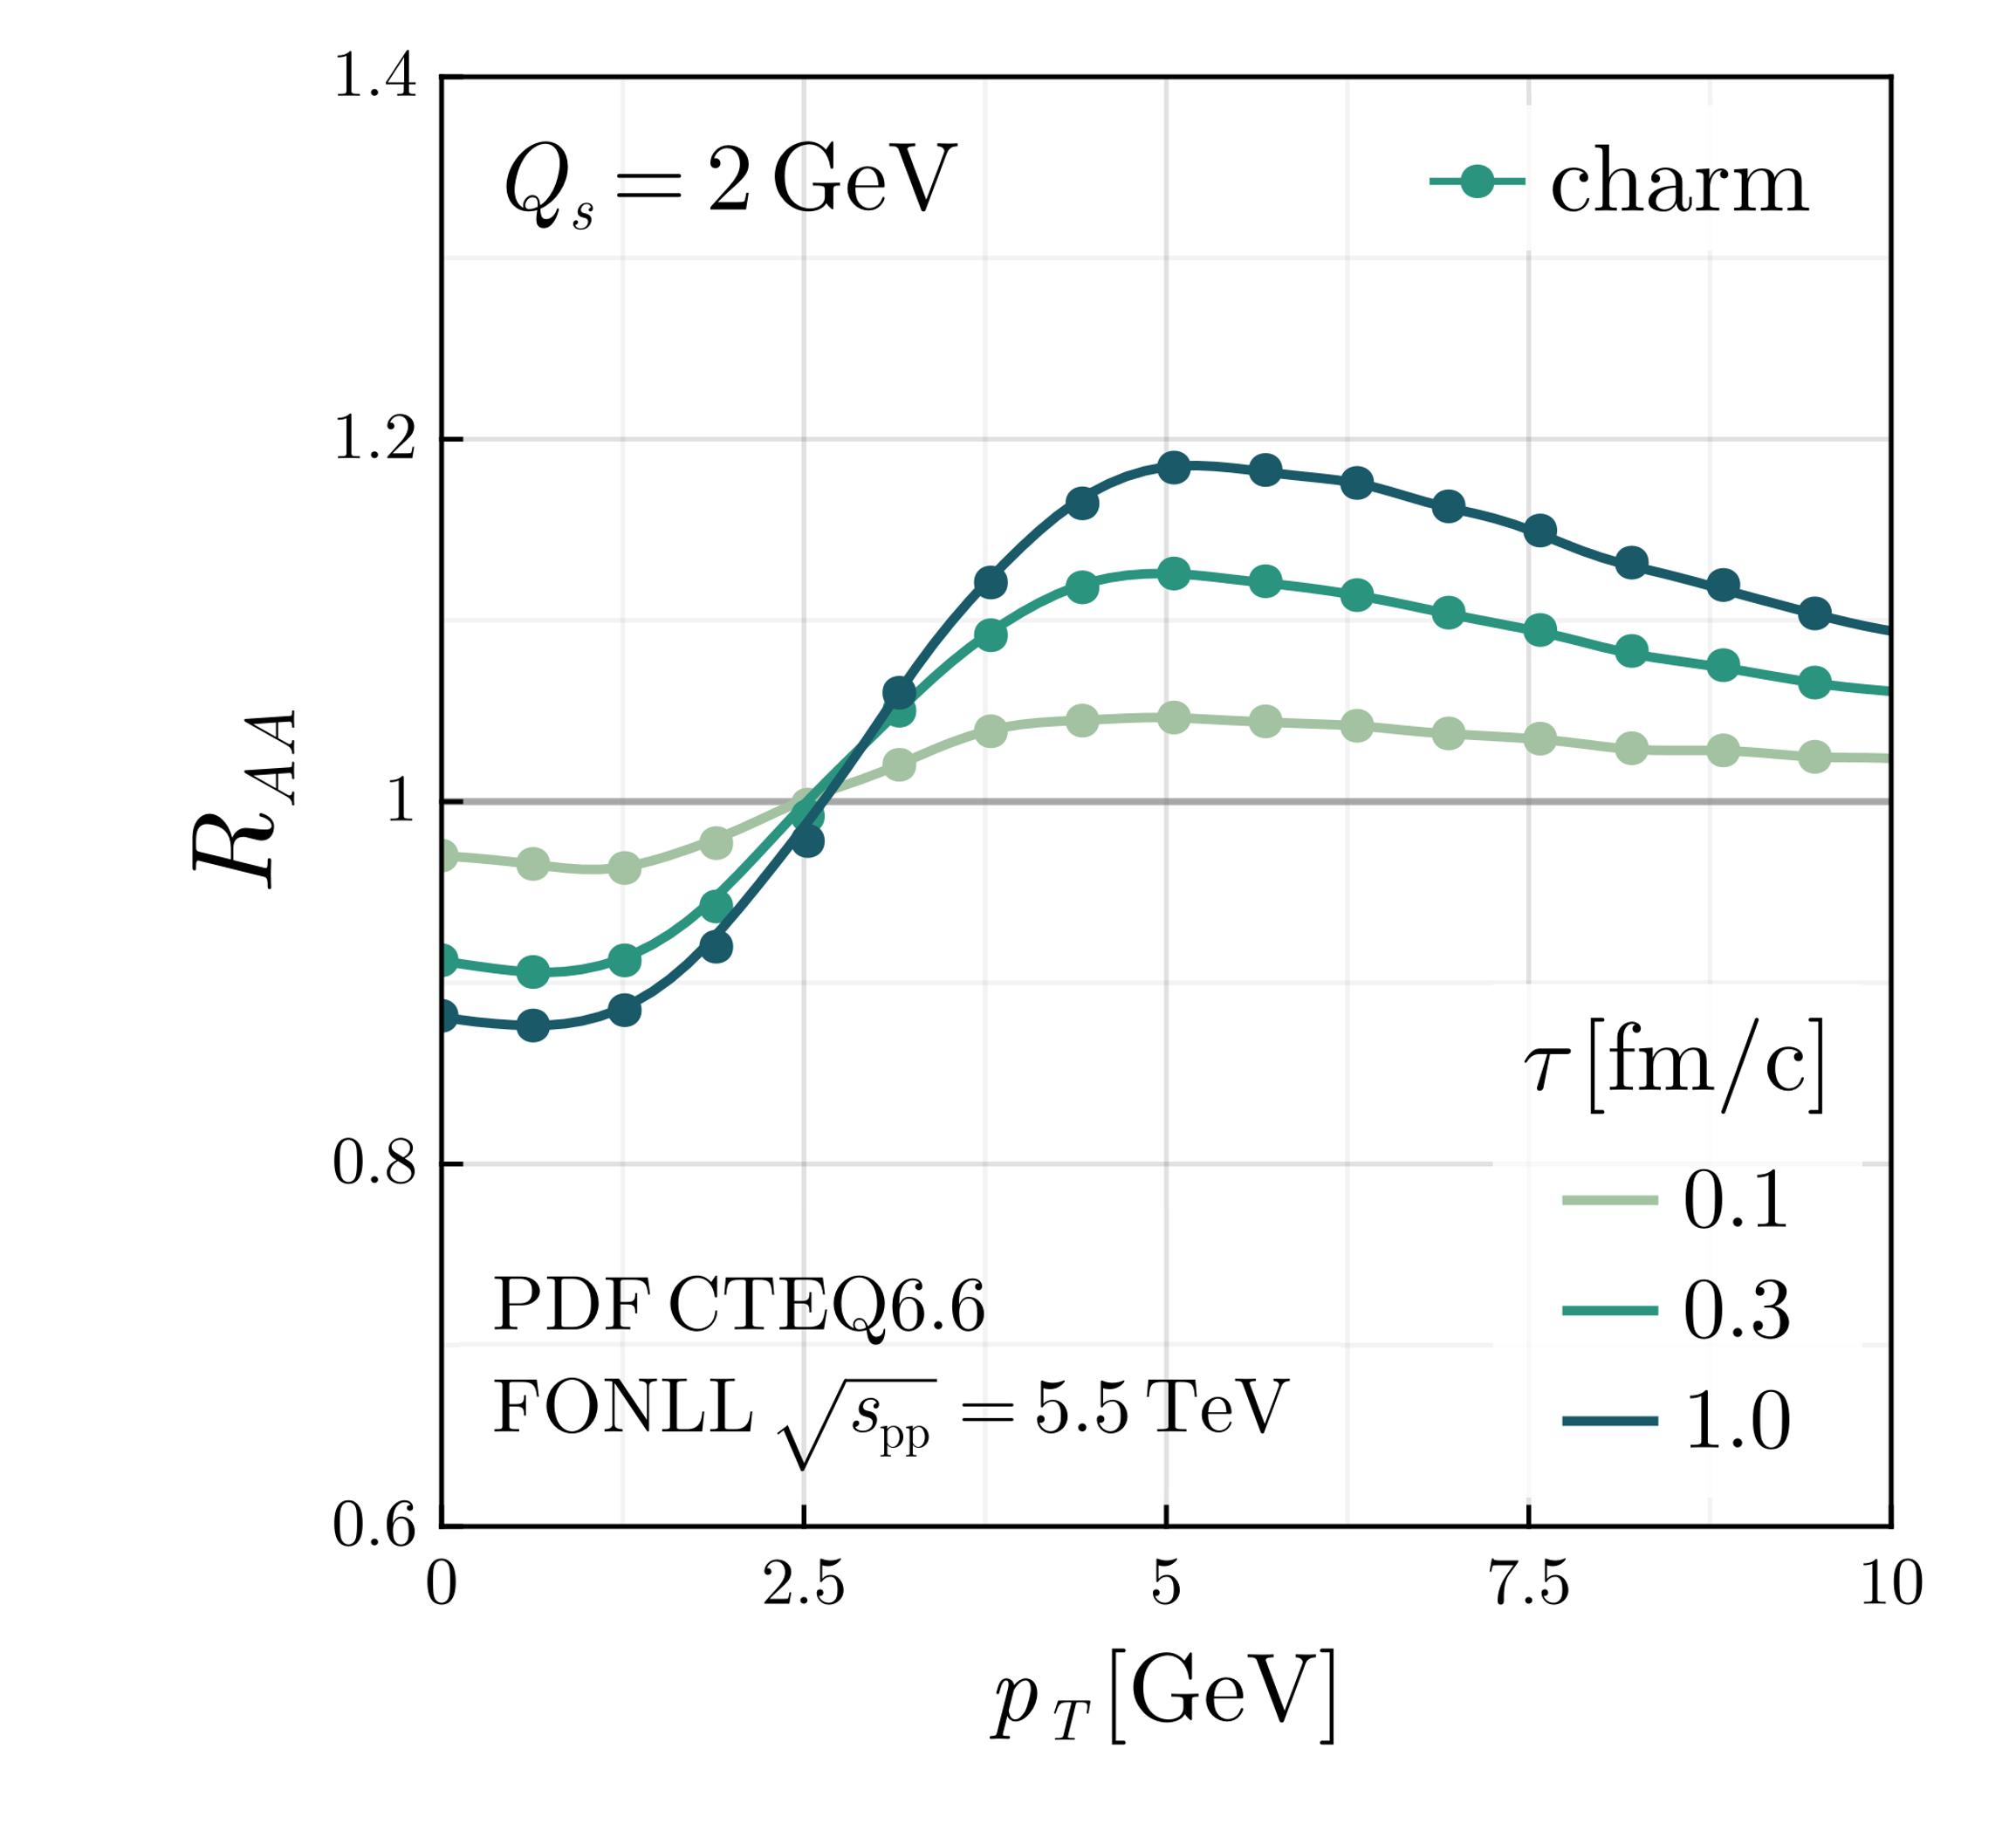
\includegraphics[width=0.9\columnwidth]{images/clean_raa_tau_dep_quarks_charmQs_2.0_fonll_energy_5500_pdf_cteq.png}
            \end{figure}
            \column{.02\textwidth}
            \column{.47\textwidth}
            \begin{center}
                \begin{custombox}{\normalsize Effect of energy scales}{raapink}
                    \small
                    \begin{varwidth}{0.95\textwidth}
                    \begin{itemize}
                        \itemsep0em
                        \footnotesize
                        \setbeamertemplate{itemize item}{\raisebox{0.2em}{\scalebox{0.7}{${\color{raapink}\blacktriangleright}$}}} 
                        \item Weak dependence on $\sqrt{s_\mathrm{pp}}$ and glasma $Q_s$
                    \end{itemize}
                    \end{varwidth}
                \end{custombox}
            \end{center}
            \vspace{-10pt}
            \vspace{-7pt}
            \begin{figure}
                \centering
                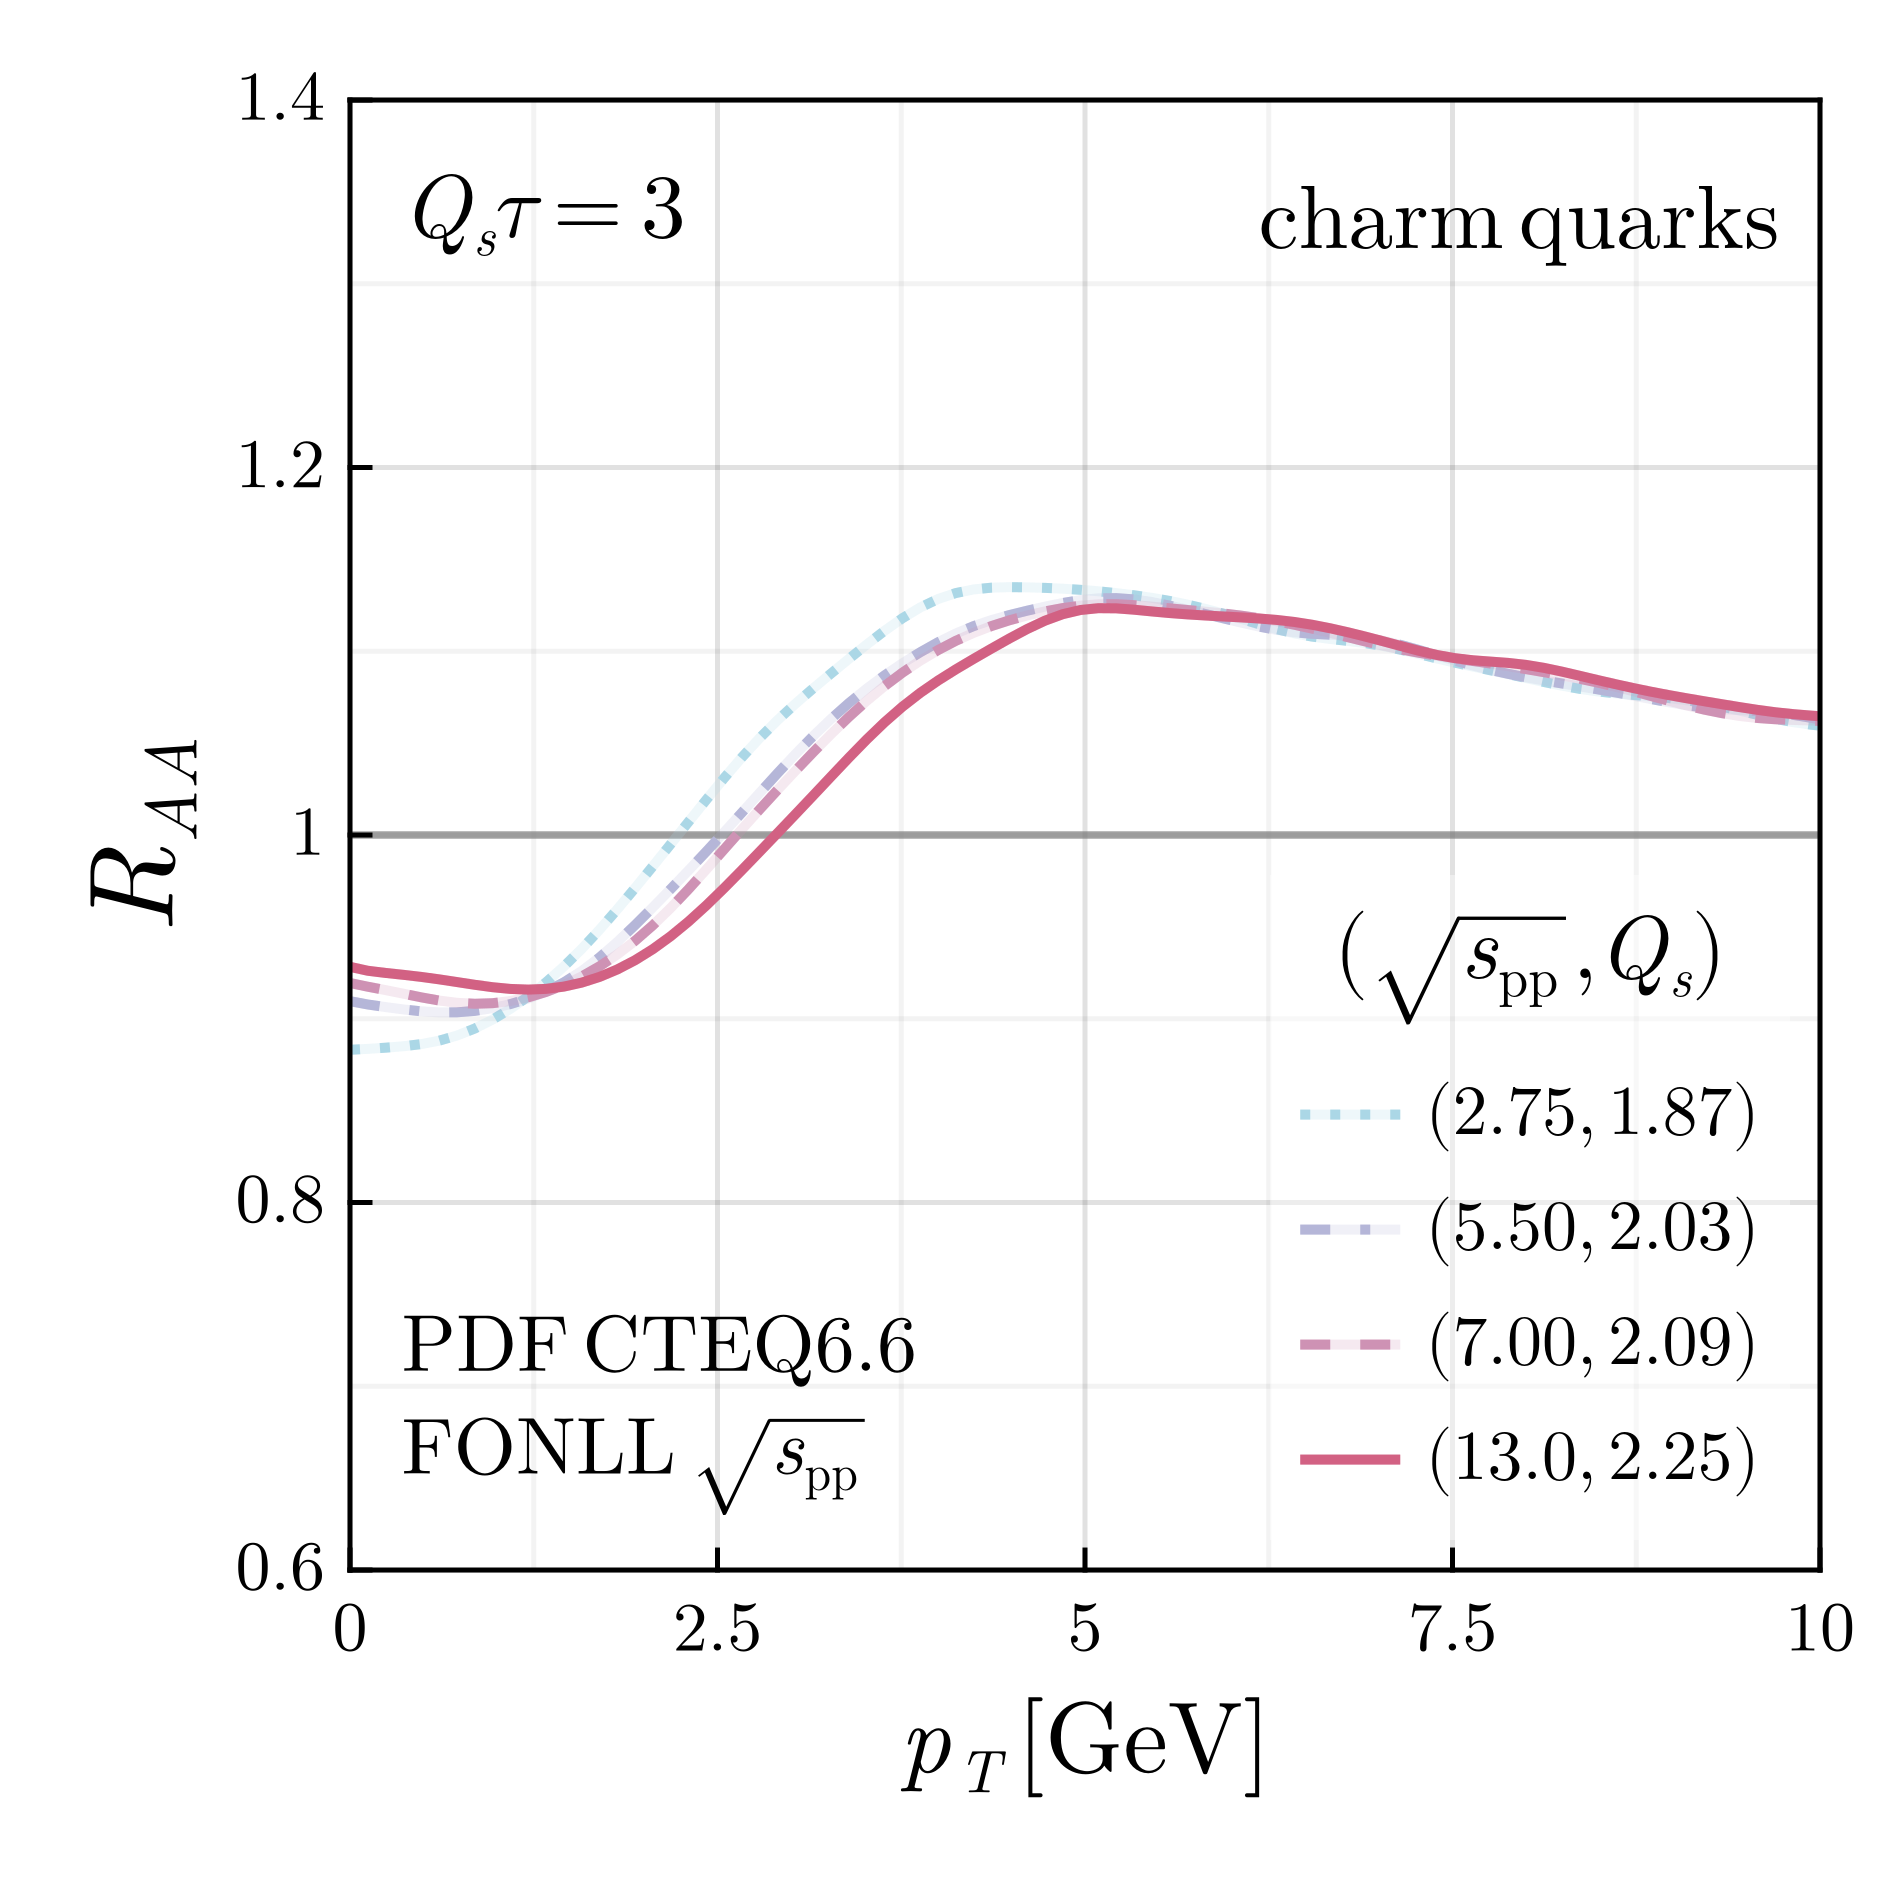
\includegraphics[width=0.83\columnwidth]{images/clean_raa_tau_dep_charm_quark_Qs_fonll_energy_dep_qsenergymap_v3.png}
            \end{figure}
            \column{.02\textwidth}
        \end{columns}    
    \end{center}
\end{frame}

%%%%%%%%%%%%%%%%%%%%%%%%%%%%%%%%%%%%%%%%%
%%%%%%%%%%%%%%%%% SLIDE %%%%%%%%%%%%%%%%%
%%%%%%%%%%%%%%%%%%%%%%%%%%%%%%%%%%%%%%%%%

\begin{frame}
    \frametitle{$R_{AA}$ in glasma with nPDFs}
    % \framesubtitle{Temporal evolution, energy dependence}
    \vspace{-15pt}
    \begin{center}
        \begin{columns}[onlytextwidth,t]
            \column{.02\textwidth}
           \column{.47\textwidth}
           \begin{center}
                \begin{custombox}{\normalsize Initial state effects}{palgold}
                    \small
                    \begin{varwidth}{0.88\textwidth}
                    \begin{itemize}
                        \itemsep0em
                        \footnotesize
                        \setbeamertemplate{itemize item}{\raisebox{0.2em}{\scalebox{0.7}{${\color{palgold}\blacktriangleright}$}}} 
                        \item No nPDF effects were considered 
                        \item Glasma $AA$ spectrum initialized with FONLL in $pp$
                    \end{itemize}
                    \end{varwidth}
                \end{custombox}
            \end{center}
            \vspace{-10pt}
           \begin{figure}
                \centering
                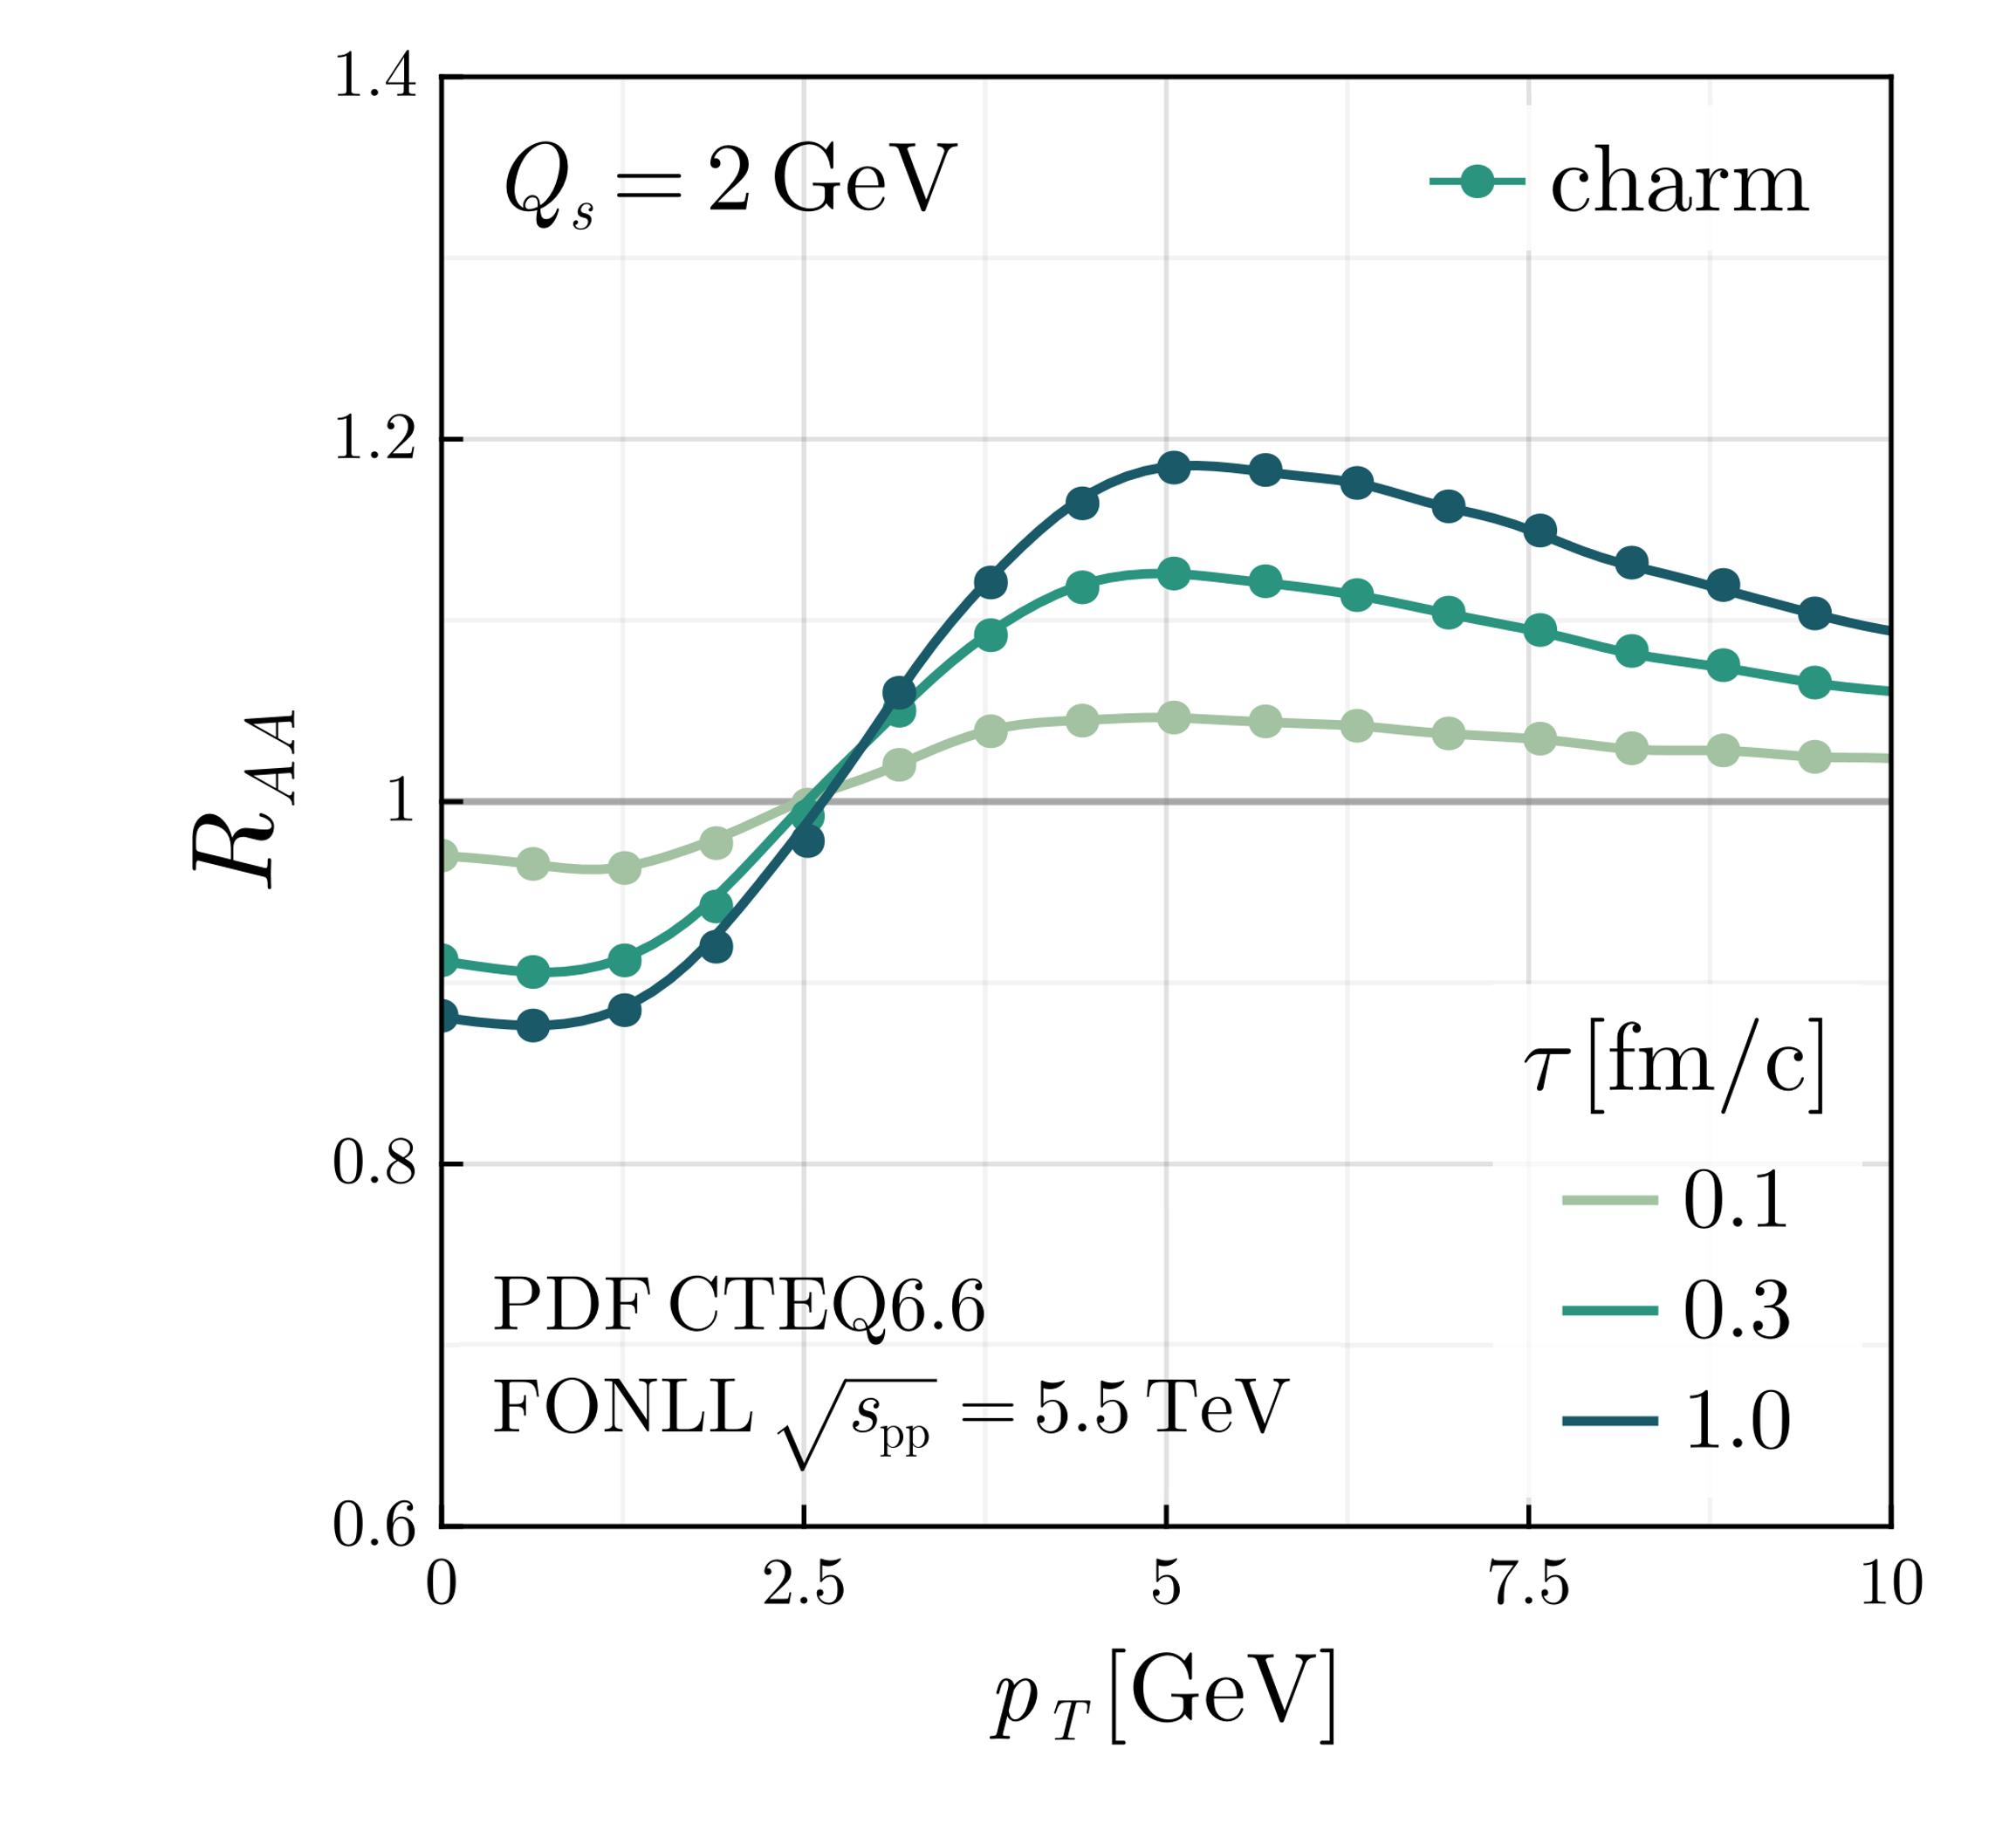
\includegraphics[width=0.9\columnwidth]{images/clean_raa_tau_dep_quarks_charmQs_2.0_fonll_energy_5500_pdf_cteq.png}
            \end{figure}
            \column{.02\textwidth}
            \column{.47\textwidth}
            \begin{center}
                \begin{custombox}{\normalsize Effect of energy scales}{raapink}
                    \small
                    \begin{varwidth}{0.95\textwidth}
                    \begin{itemize}
                        \itemsep0em
                        \footnotesize
                        \setbeamertemplate{itemize item}{\raisebox{0.2em}{\scalebox{0.7}{${\color{raapink}\blacktriangleright}$}}} 
                        \item Weak dependence on $\sqrt{s_\mathrm{pp}}$ and glasma $Q_s$
                    \end{itemize}
                    \end{varwidth}
                \end{custombox}
            \end{center}
            \vspace{-10pt}
            \vspace{-7pt}
            \begin{figure}
                \centering
                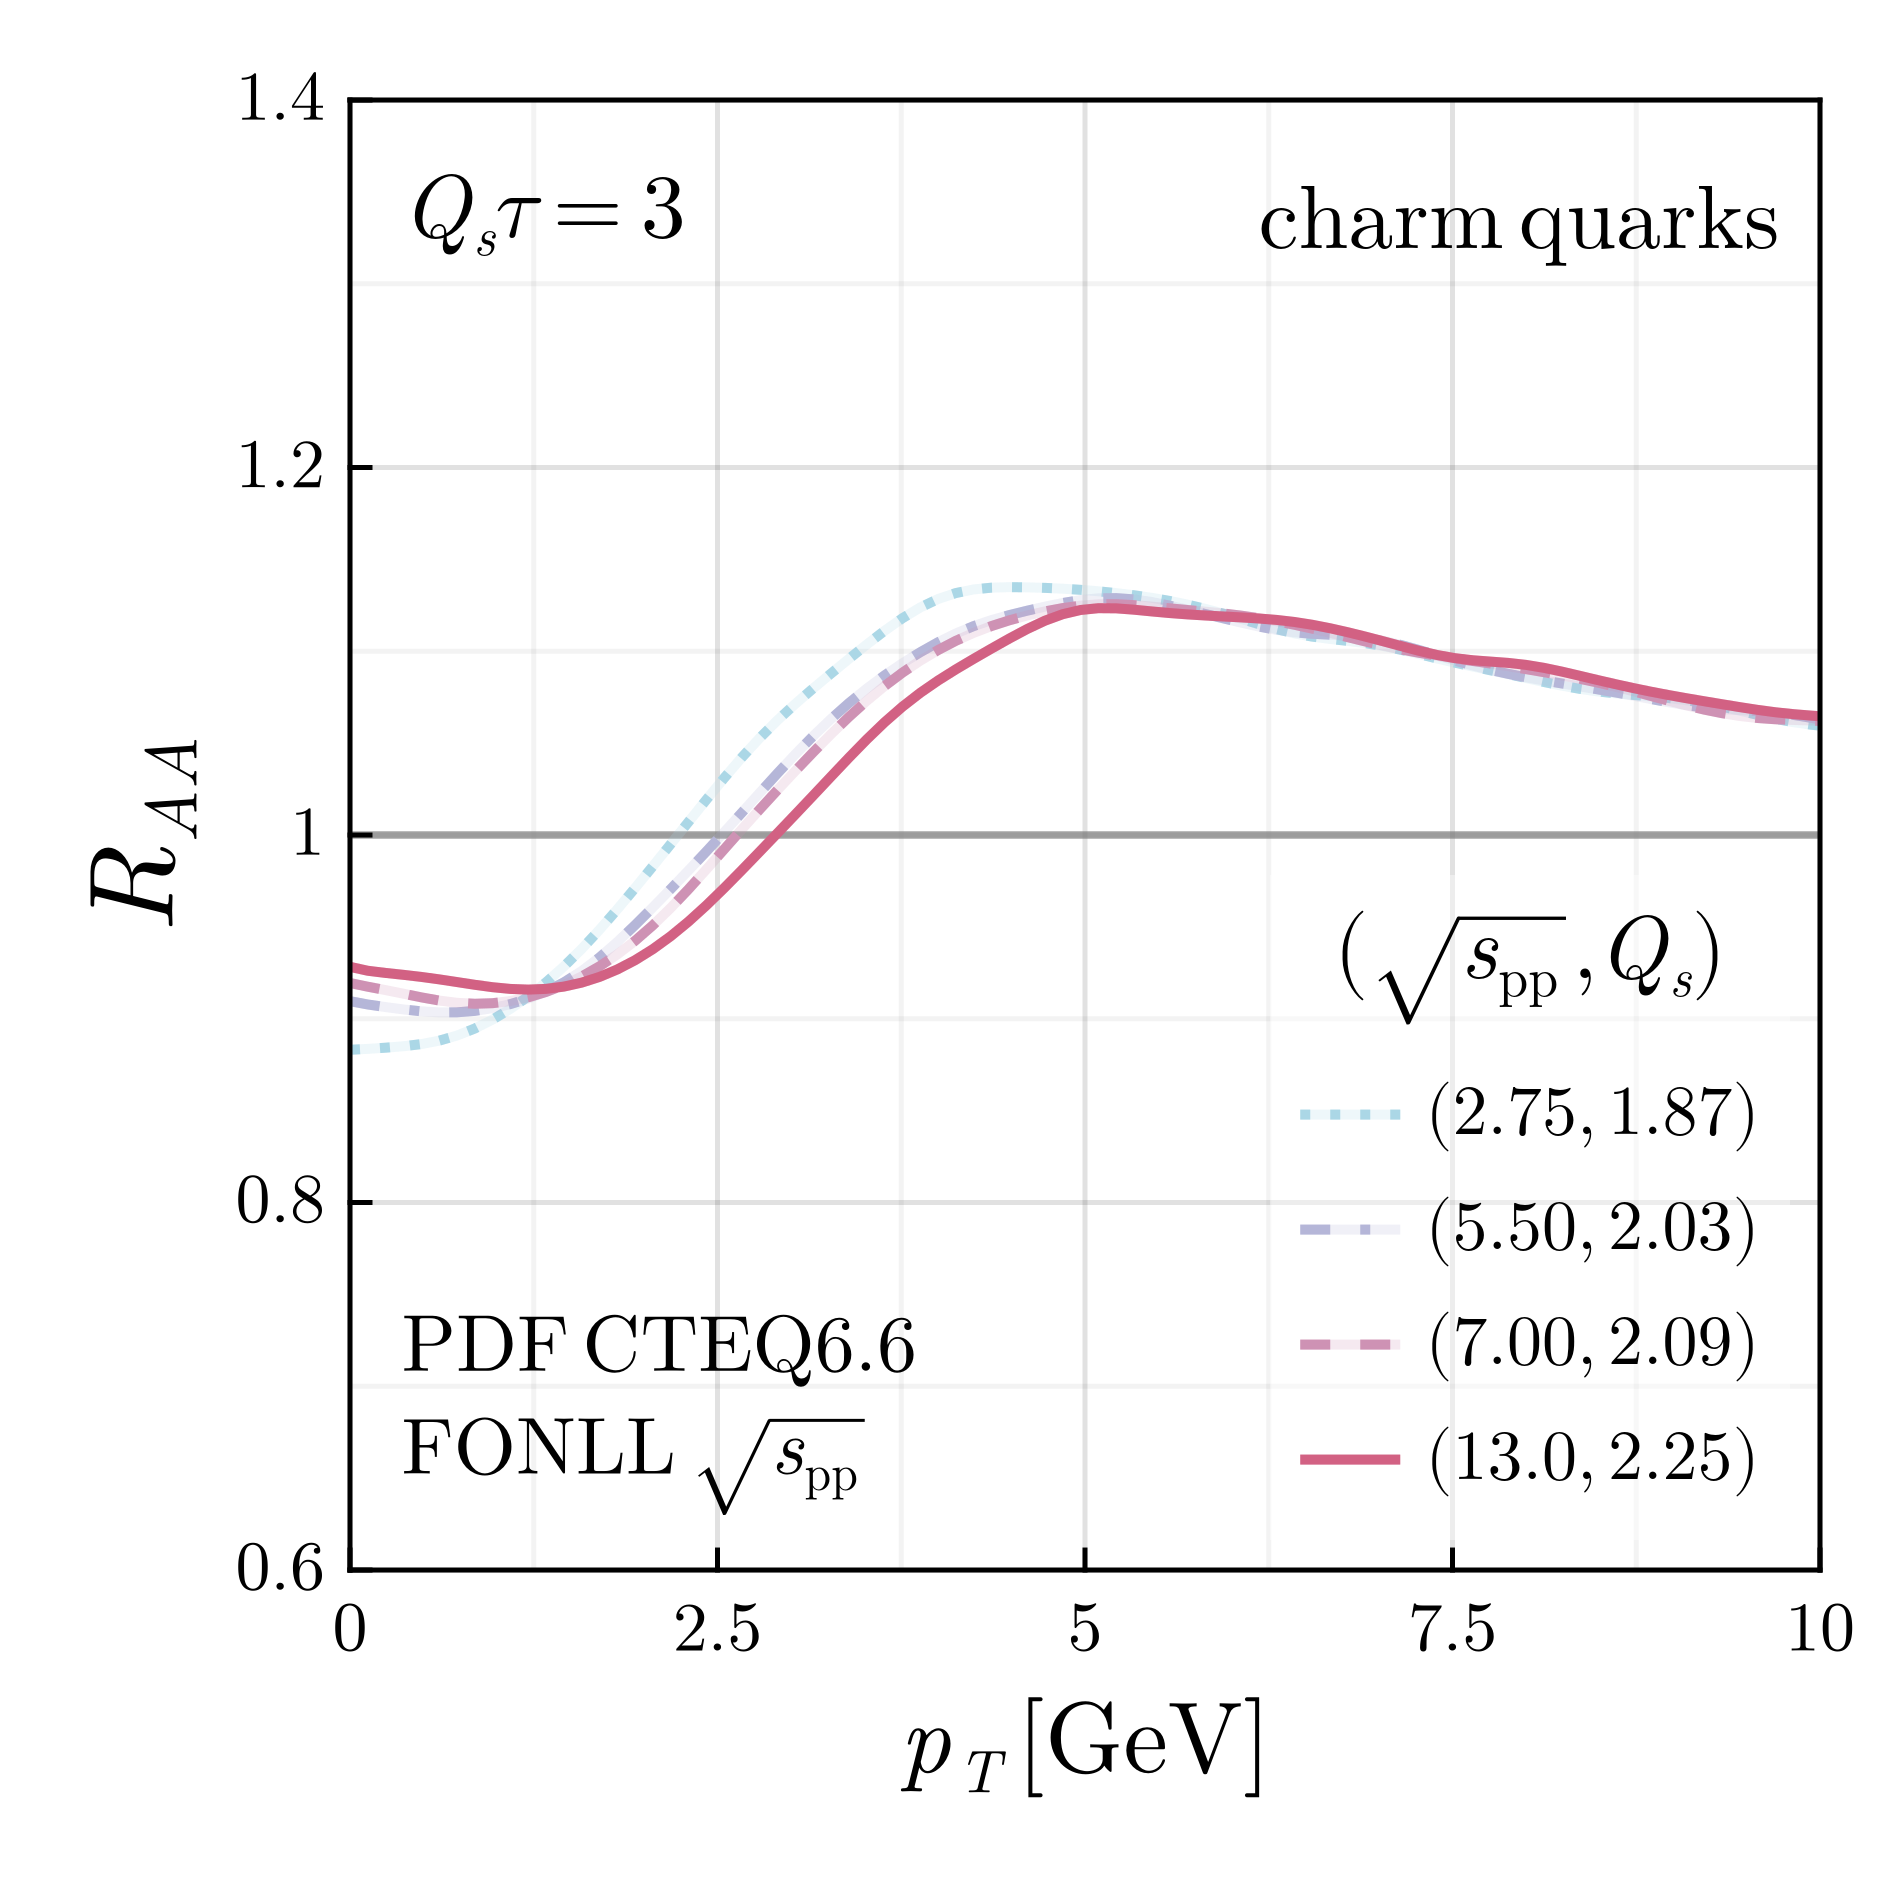
\includegraphics[width=0.83\columnwidth]{images/clean_raa_tau_dep_charm_quark_Qs_fonll_energy_dep_qsenergymap_v3.png}
            \end{figure}
            \column{.02\textwidth}
        \end{columns}    
    \end{center}
\end{frame}

%%%%%%%%%%%%%%%%%%%%%%%%%%%%%%%%%%%%%%%%%
%%%%%%%%%%%%%% SUBSECTION %%%%%%%%%%%%%%%
%%%%%%%%%%%%%%%%%%%%%%%%%%%%%%%%%%%%%%%%%

\subsection{Two-particle correlations}

\end{document}